%%%%HEADER
\documentclass[twocolumn]{article}
\usepackage[a4paper, margin=1in, columnsep=20pt]{geometry}
\usepackage{amsmath, amssymb, graphicx, hyperref}
\usepackage[most,skins,breakable]{tcolorbox}
\usepackage[symbol]{footmisc}
\usetikzlibrary{calc}
\usepackage{xcolor}
\usepackage{caption}
\usepackage{algorithm}
\usepackage{algpseudocodex}
\usepackage{tikz}
\usepackage{listings}
\usetikzlibrary{arrows.meta, positioning}
\tcbuselibrary{listingsutf8}
\usepackage{microtype}
\usepackage{blindtext}
\usepackage{bookmark}
\usepackage{breqn}
\usepackage[backend=biber,style=numeric]{biblatex} % 
\addbibresource{../references.bib}

% Define style for the listings environment
\lstdefinestyle{mystyle}{
    basicstyle=\ttfamily\small,
    breaklines=true,
    escapeinside={(*@}{@*)}, % Allows math mode within listings
    numbers=left,
    numberstyle=\tiny,
    frame=single,
    keywordstyle=\color{blue}\bfseries,
    commentstyle=\color{green!50!black},
    stringstyle=\color{red}
}


\def\reals{\mathbb{R}}
% Define the custom definition box and command
\newtcolorbox{mydefinition}[2][]{%
    text width=0.95\columnwidth,
    before=\vspace{1mm}, 
    after=\vspace{1mm}, 
    colback=gray!10, % Background color (light gray)
    colframe=black!70,  % Border color
    coltitle=gray!10,  % Title color
    fonttitle=\bfseries, % Title font style
    sharp corners,   % Box style
    left=2pt,
    breakable,
    right=2pt,
    top=2pt,
    bottom=2pt,
    enhanced jigsaw,
    title=Definition: {#1},         % Title passed as the first argument
    colupper=black,  % Ensure proper content handling
    pad at break*=1pc,
    overlay first and middle={
        \coordinate (A1) at ($(interior.south east) + (-10pt,5pt)$);
        \coordinate (C1) at ($(interior.south east) + (-6pt,7.5pt)$);
        \draw[fill=black!50] (A1) -- +(0,5pt) -- (C1) -- cycle;
    }
    }
    
\newcommand{\definition}[2]{%
    \noindent%
    \begin{mydefinition}[#1]%
        .#2%
    \end{mydefinition}%
    \noindent
}

\newtcolorbox{myexample}[2][]{%
    text width=0.95\columnwidth,
    before=\vspace{1mm}, 
    after=\vspace{1mm}, 
    colback=orange!3, % Background color (light gray)
    colframe=black!70,  % Border color
    coltitle=gray!10,  % Title color
    fonttitle=\bfseries, % Title font style
    sharp corners,   % Box style
    left=2pt,
    right=2pt,
    top=2pt,
    bottom=2pt,
    breakable,
    title=Intuition: {#1},         % Title passed as the first argument
    pad at break*=1pc,
    overlay first and middle={
        \coordinate (A1) at ($(interior.south east) + (-10pt,5pt)$);
        \coordinate (C1) at ($(interior.south east) + (-6pt,7.5pt)$);
        \draw[fill=black!50] (A1) -- +(0,5pt) -- (C1) -- cycle;
    }
}

\newcommand{\example}[2]{%
    \noindent%
    \begin{myexample}[#1]%
    .#2%
    \end{myexample}%
    \noindent
}

\newtcolorbox{algobox}[2][]{%
    text width=0.95\columnwidth,
    before=\vspace{1mm}, 
    after=\vspace{1mm}, 
    colback=blue!5, % Background color (light gray)
    colframe=black!70,  % Border color
    coltitle=gray!10,  % Title color
    fonttitle=\bfseries, % Title font style
    sharp corners,   % Box style
    left=2pt,
    right=2pt,
    top=2pt,
    bottom=2pt,
    breakable,
    title=Algorithm: {#1},         % Title passed as the first argument
    pad at break*=1pc,
    overlay first and middle={
        \coordinate (A1) at ($(interior.south east) + (-10pt,5pt)$);
        \coordinate (C1) at ($(interior.south east) + (-6pt,7.5pt)$);
        \draw[fill=black!50] (A1) -- +(0,5pt) -- (C1) -- cycle;
    }
}

\newcommand{\algorithmbox}[2]{%
\noindent%
    \begin{algobox}[#1]%
    .#2%
    \end{algobox}%
    \noindent
}
%%%%HEADER

\def\COMPILINGFROMMAIN{}
\begin{document}
\title{\Huge{Probabilistic Numerical Solvers for Partial Differential Equations on Riemannian 2-Manifolds}}
\author{
\\
Master's Thesis in Computer Science
\\
\\
\\
\\
\\
\\
\\
Theo Rüter Würtzen\vspace{2mm}
\\
Department of Computer Science
\\
University of Copenhagen
\\
\\
\\
\\
\\
\\
\\
\\
\\
Supervised by 
\\
\\
\\
\\
\\
Peter Nicholas Krämer\vspace{2mm}
\\
Section for Cognitive Systems
\\
Technical University of Denmark
\\
\\
\\
\\
\hspace*{7mm}\begin{tabular}{ccc}
    \begin{tabular}{c}
        Søren Hauberg\vspace{2mm}
\\
Section for Cognitive Systems
\\
Technical University of Denmark
    \end{tabular}
     & & \begin{tabular}{c}
        Sebastian Weichwald\vspace{2mm}
\\
Department of Mathematical Sciences
\\
University of Copenhagen
    \end{tabular}
\end{tabular}
}
\date{}
\maketitle

\clearpage


\begin{abstract}
Partial differential equations are ubiquitous in physics and simulations, and generally have to be solved numerically. The field of probabilistic numerics focuses on framing computation as probabilistic inference and has led to the development of efficient and competitive probabilistic numerical solvers of ordinary differential equations, which give the solution as a stochastic process. In this thesis, we extend the use of these solvers to partial differential equations on Riemannian manifolds. We give introductions to the touched upon topics, including but not limited to discretization of Riemannian manifolds, the associated discrete differential operators, and the use of stochastic differential equations as priors. We give an algorithm to build an intrinsic triangulation of a manifold, and empirically demonstrate how certain priors can accelerate the process of solving nonlinear PDEs. We have structured the thesis as a high level guide on how to implement and follow the results, and we try to motivate the steps to the best of our efforts. We teach and explain with a focus on giving intuition through examples and analogies, and provide pointers to further reading.
\end{abstract}

\section*{Acknowledgements}
I thank Nicholas for his high availability and thorough eye for detail during every supervision session and for including me in the fun sessions at the research group. I thank Søren Hauberg and Sebastian Weichwald for their enthusiasm and for enabling this project. Finally, I pat myself on the back for putting in a lot of work.

\newpage
\tableofcontents
\newpage
\section{Overview}\label{sec:overview}
The thesis can broadly be seen as consisting of two separate parts that meet towards the end. One deals with Riemannian manifolds and how to convert them to a discrete form amenable to numerical computation. The other deals with ordinary / partial / stochastic differential equations and probabilistic numerical solvers. Finally these two parts converge, and we will use the discrete Laplacian and the probabilistic numerical solvers to solve partial differential equations whose spatial domain is the manifold.
\\
The thesis touches upon many subjects, some of which are active areas of research and could have been an entire thesis by themselves. We will supplement what is not taught in a classic computer / data science curriculum, but a full coverage of the topics is beyond the scope of this thesis. Nearly all figures in the thesis were made during the project and have subsequently been included in the thesis because they were found to be helpful in understanding the topics. 
\\The main parts of the thesis are structured as follows:
\\\\
Chapter \ref{sec:background} is the most verbose part of the thesis and serves to get the reader into the mood and right mindset for the rest of the thesis. It gives a brief introduction to the field of probabilistic numerics and further motivates the topics of the thesis.
\\\\
Chapter \ref{sec:manifolds} gives an applied introduction to Riemannian manifolds, triangle meshes and the discrete exterior calculus, all with the intention of defining the discrete Laplacian on a discrete manifold.
\\\\
Chapter \ref{sec:intrinsic_triangulation} builds on chapter \ref{sec:manifolds} and addresses the problem of building the Laplacian matrix given only a Riemannian metric. We contribute an algorithm that solves this problem by constructing an intrinsic triangulation of a manifold, from which one can then build the Laplacian matrix using the tools from \ref{sec:manifolds}. We demonstrate the algorithm on a few examples.
\\\\
Chapter \ref{sec:pde} is the second part of the thesis. It gives an introduction to ordinary and partial differential equations. We discuss the ideas of the state-space representation and discretization using the Method of Lines, which is the principle we will use in the later probabilistic numerical solver.
\\\\
Chapter \ref{sec:prior} builds on chapter \ref{sec:pde} to introduce the probabilistic numerical solver for ordinary differential equations. We will cover how to specify a prior distribution over the solution using a stochastic differential equation, show how to manipulate the prior and posterior probability distributions, and give specific pointers on how to implement a stable solver.
\\\\
Chapter \ref{sec:solver_experiments} wraps up with a demonstration of the solver on a few examples. We show how the solver can be used to solve nonlinear PDEs, and contribute problem-specific priors that improve the speed of convergence.

\section{Background}\label{sec:background}

\subsection*{Probabilistic Numerical Methods}
The field of probabilistic numerics methods frames traditional numerical tasks as problems of probabilistic inference. This approach enables the explicit modeling of uncertainty arising from limited computational resources \cite{itergp}, discretization errors \cite{pnmol}, or incomplete information \cite{exponential_probabilistic}. The book \cite{probnum} is a comprehensive introduction to the field. Probabilistic numerics has yielded Bayesian approaches to solutions of linear algebra problems \cite{pn_solver}, optimization problems \cite{pn_optimization}, and differential equations \cite{invention_of_ODE_solver}, leading to algorithms capable of not only producing a solution but also quantifying the uncertainty in that solution. Given prior beliefs about the unknown solution and a likelihood model informed by computational observations (e.g., evaluations of a differential operator), probabilistic solvers infer a posterior distribution over the solution.


\subsection*{Numerical Solvers for Differential Equations}
Traditional numerical methods for solving differential equations, such as the Runge-Kutta \cite{runge} methods, produce deterministic approximations of the solution. One can choose a trade-off between accuracy and computational efficiency \cite{butcher}, expressed by the convergence rate \cite{kanschat} of the method.

On the other hand, Probabilistic Numerical solvers represent the solution as a distribution of functions \cite{nicoThesis} parameterized by a Gaussian process \cite{gp_Rasmussen}. Instead of providing a single point estimate of the solution, these solvers return a probability distribution that encapsulates the uncertainty over the solution. Using a probabilistic solver necessitates the choice of a prior distribution over the solution, which affects the behaviour of the solver. This is not a drawback, but a feature, as the choice of prior can encode prior knowledge about the solution, such as smoothness or periodicity \cite{gp_Rasmussen}. 

\subsection*{Why Uncertainty Quantification?}

The uncertainty of a solution is often seen as a by-product of the numerical method, but it serves as an important enabler for dynamic decision-making, especially in safety-critical applications. For example, in a medical setting, it would allow doctors to manually prescribe a treatment or get third opinions if the model shows uncertainty about its diagnosis. 
At its best, it allows reasoning about the range of possible outcomes to further propagate the uncertainty through later stages of a system.
\\
Active learning \cite{active_learning} is a field in which modeling uncertainty plays a big role. Under a limited budget, one can optimize to reduce uncertainty about some quantity of interest. In machine learning, it serves to identify regions of data where models are prone to errors, and can guide data collection \cite{safeopt}. In \cite{pnmol}, the authors model the uncertainty of spatial and temporal discretization errors in probabilistic numerical solvers of ODEs, which enables prioritized discretization where it will bring the most benefit. 
To truly be able to rely on uncertainty quantification, it must be calibrated, meaning that the uncertainty should be a good estimate of the true uncertainty. Fortunately, \cite{calibrated_probabilistic} show that probabilistic solvers of ODEs do indeed provide well- calibrated uncertainty estimates.

\subsection*{Why Differential Equations?}

Differential equations (DEs) play a central role in the natural sciences as tools for modeling and understanding dynamic systems. They describing the evolution of systems over time and/or space and are commonly found in physics, biology, engineering and even finance. In physics, famously Schrödinger's equation models the quantum state of a system, and the Navier-Stokes equations model fluid flow. In the earth sciences, models of climate systems rely on multiple sets of DEs. In biology, reaction-diffusion equations describe processes like morphogenesis\footnote{This is the process that leads to biological cells having a specific shape.}. Modeling uncertainties here is also useful - an example that comes to mind is the chance-of-rain\footnote{Apparently, this is formally known as "Probability of precipitation" } in a weather forecast, or the uncertainty in the prediction of a stock price. 

\subsection*{Differential Equations in Machine Learning}
Differential equations are also finding increasing relevance in machine learning \cite{neuralode} \cite{diffrax}. Neural ODEs enable learning continuous-time models of data, offering a more flexible alternative to discrete-time approaches like the RNN \cite{rnn}. This has led to the rise of physics-informed neural networks \cite{pinn} that are trained to satisfy some specific DE. Diffusion models \cite{diffusion} and normalizing flows \cite{nflow} are examples of probabilistic generative models that leverage the language of DEs to define complex distributions.
Generally, these approaches require some form of a numerical solver of DEs, and using probabilistic solvers can provide an alternative to the standard ones if calibrated uncertainty estimates are needed.
\subsection*{Manifolds in Machine Learning}
Riemannian manifolds provide a mathematical framework for studying curved spaces, generalizing the notion of Euclidean geometry ($\reals^n$) to non-Euclidean settings. They serve also as domains for constrained optimization problems \cite{gaussian_robot}. Some data is not naturally represented well in a Euclidean space, the simplest example being angles, which wrap around. Another example is the manifold of positive semidefinite matrices \cite{pymanopt}, useful when fitting Gaussian mixture models.
The link between probabilistic numerical solvers and manifolds has been made before in \cite{hennig2014probabilistic} where the authors compute geodesics (shortest paths) on manifolds using probabilistic solvers. In machine learning, taking into account the geometry of the data can make simple models competitive \cite{hauberg2012geometric} and lead to higher interpretability \cite{arvanitidis2017latent}.

\subsection*{Why the Focus on 2-Manifolds}
When one could have chosen to work with 4-dimensional manifolds, choosing 2-dimensional manifolds can seem like a boring choice. Although the continuous mathematical description of manifolds is mature well beyond 2 dimensions, the discrete counterparts are not as well-developed\cite{craneDDG}. Triangle meshes are a common discretization of manifolds, and in 3D finite-element methods one will encounter the tetrahedral mesh. 2-dimensions are a good starting point because they can be visualized and there are lots of interesting problems to solve in 2D \cite{walk_on_stars} \cite{repulsive_curves} \cite{diffusionnet}. 


\clearpage
\section{Riemannian Manifolds and Discrete Exterior Calculus}\label{sec:manifolds}
\ifdefined\COMPILINGFROMMAIN
\else
    %%%%HEADER
\documentclass[twocolumn]{article}
\usepackage[a4paper, margin=1in, columnsep=20pt]{geometry}
\usepackage{amsmath, amssymb, graphicx, hyperref}
\usepackage[most,skins,breakable]{tcolorbox}
\usepackage[symbol]{footmisc}
\usetikzlibrary{calc}
\usepackage{xcolor}
\usepackage{caption}
\usepackage{algorithm}
\usepackage{algpseudocodex}
\usepackage{tikz}
\usepackage{listings}
\usetikzlibrary{arrows.meta, positioning}
\tcbuselibrary{listingsutf8}
\usepackage{microtype}
\usepackage{blindtext}
\usepackage{bookmark}
\usepackage{breqn}
\usepackage[backend=biber,style=numeric]{biblatex} % 
\addbibresource{../references.bib}

% Define style for the listings environment
\lstdefinestyle{mystyle}{
    basicstyle=\ttfamily\small,
    breaklines=true,
    escapeinside={(*@}{@*)}, % Allows math mode within listings
    numbers=left,
    numberstyle=\tiny,
    frame=single,
    keywordstyle=\color{blue}\bfseries,
    commentstyle=\color{green!50!black},
    stringstyle=\color{red}
}


\def\reals{\mathbb{R}}
% Define the custom definition box and command
\newtcolorbox{mydefinition}[2][]{%
    text width=0.95\columnwidth,
    before=\vspace{1mm}, 
    after=\vspace{1mm}, 
    colback=gray!10, % Background color (light gray)
    colframe=black!70,  % Border color
    coltitle=gray!10,  % Title color
    fonttitle=\bfseries, % Title font style
    sharp corners,   % Box style
    left=2pt,
    breakable,
    right=2pt,
    top=2pt,
    bottom=2pt,
    enhanced jigsaw,
    title=Definition: {#1},         % Title passed as the first argument
    colupper=black,  % Ensure proper content handling
    pad at break*=1pc,
    overlay first and middle={
        \coordinate (A1) at ($(interior.south east) + (-10pt,5pt)$);
        \coordinate (C1) at ($(interior.south east) + (-6pt,7.5pt)$);
        \draw[fill=black!50] (A1) -- +(0,5pt) -- (C1) -- cycle;
    }
    }
    
\newcommand{\definition}[2]{%
    \noindent%
    \begin{mydefinition}[#1]%
        .#2%
    \end{mydefinition}%
    \noindent
}

\newtcolorbox{myexample}[2][]{%
    text width=0.95\columnwidth,
    before=\vspace{1mm}, 
    after=\vspace{1mm}, 
    colback=orange!3, % Background color (light gray)
    colframe=black!70,  % Border color
    coltitle=gray!10,  % Title color
    fonttitle=\bfseries, % Title font style
    sharp corners,   % Box style
    left=2pt,
    right=2pt,
    top=2pt,
    bottom=2pt,
    breakable,
    title=Intuition: {#1},         % Title passed as the first argument
    pad at break*=1pc,
    overlay first and middle={
        \coordinate (A1) at ($(interior.south east) + (-10pt,5pt)$);
        \coordinate (C1) at ($(interior.south east) + (-6pt,7.5pt)$);
        \draw[fill=black!50] (A1) -- +(0,5pt) -- (C1) -- cycle;
    }
}

\newcommand{\example}[2]{%
    \noindent%
    \begin{myexample}[#1]%
    .#2%
    \end{myexample}%
    \noindent
}

\newtcolorbox{algobox}[2][]{%
    text width=0.95\columnwidth,
    before=\vspace{1mm}, 
    after=\vspace{1mm}, 
    colback=blue!5, % Background color (light gray)
    colframe=black!70,  % Border color
    coltitle=gray!10,  % Title color
    fonttitle=\bfseries, % Title font style
    sharp corners,   % Box style
    left=2pt,
    right=2pt,
    top=2pt,
    bottom=2pt,
    breakable,
    title=Algorithm: {#1},         % Title passed as the first argument
    pad at break*=1pc,
    overlay first and middle={
        \coordinate (A1) at ($(interior.south east) + (-10pt,5pt)$);
        \coordinate (C1) at ($(interior.south east) + (-6pt,7.5pt)$);
        \draw[fill=black!50] (A1) -- +(0,5pt) -- (C1) -- cycle;
    }
}

\newcommand{\algorithmbox}[2]{%
\noindent%
    \begin{algobox}[#1]%
    .#2%
    \end{algobox}%
    \noindent
}
%%%%HEADER

    \begin{document}
\fi
This section covers relevant knowledge of Riemannian 2-Manifolds by motivating and explaining key concepts through definitions and examples. The intention is to give intuition and working knowledge relating to later applications and algorithms. The definitions will stick to 2-manifolds, but the definitions and ideas will carry into higher (or lower) dimensions with the same principles. 
We then move to the theory of Discrete Exterior Calculus, which provides us with a principled way of computing a discrete differential operators. We will focus on the topics that lead up to the Laplacian, which will be central to the PDEs we will be solving.

\section*{Riemannian 2-Manifolds}

For millenia society thought that earth was a flat, because that's what it looks like up close. If we model earth as a unit-ball, then its surface, the unit-sphere, looks locally flat. Mathematically, we say that each point on the sphere is locally topologically equivalent (homeomorphic) to $\reals^2$.

\definition{Manifold}{
    An n-manifold is a topological space with the property that each point has a neighborhood that is homeomorphic to an open subset of $\reals^n$.    
}
Although the surface of the earth lies in our physical 3-dimensional space, we humans have found a way to parametrize it in terms of just two numbers, latitude and longitude, which yield a local representation. The Equirectangular projection maps the sphere to $[-\pi/2, \pi/2) \times [-\pi, \pi]$, which are spherical coordinates that correspond exactly to the geographical coordinates $\text{Lat}^\circ$ and $\text{Lon}^\circ$. One might erroneously have thought that this was what the Mercator projection does, but the latter will stretch the latitude near the two poles for good reasons.
%[INSERT PICTURE OF EQUIRECTANGULAR MAP https://en.wikipedia.org/wiki/Equirectangular_projection]
    
    
\definition{Coordinate Chart}{
    A 2D coordinate chart of $\mathcal{M}$ is a pair $(C, f)$, where $f$ is a diffeomorphism\footnote{A diffeomorphism is a bijection between two differentiable manifolds such that both it and its inverse are continuous. Strictly speaking, a homeomorphism is enough here (meaning not necessarily differentiable), but since we are ultimately interested in doing calculus on our manifold, we need a differentiable representation of it.} $$f: U \to C$$ that maps open subset $U$ of a 2-manifold $\mathcal{M}$ to an open subset $C \subseteq \reals^2$, resulting in a real-vector space representation of $U$.
}
\example{Coordinate Chart}{
    We will use the surface of the earth as $\mathcal{M}$ and construct a our own coordinate chart. For simplicity, we are modeling it as a unit-sphere and will only be mapping the open\footnote{This means we exclude the equator.} upper hemisphere $\subset \mathcal{M}$ to the open unit-disc $C$ by projecting the hemisphere onto the unique plane that cuts through the equator. 
    \begin{center}
        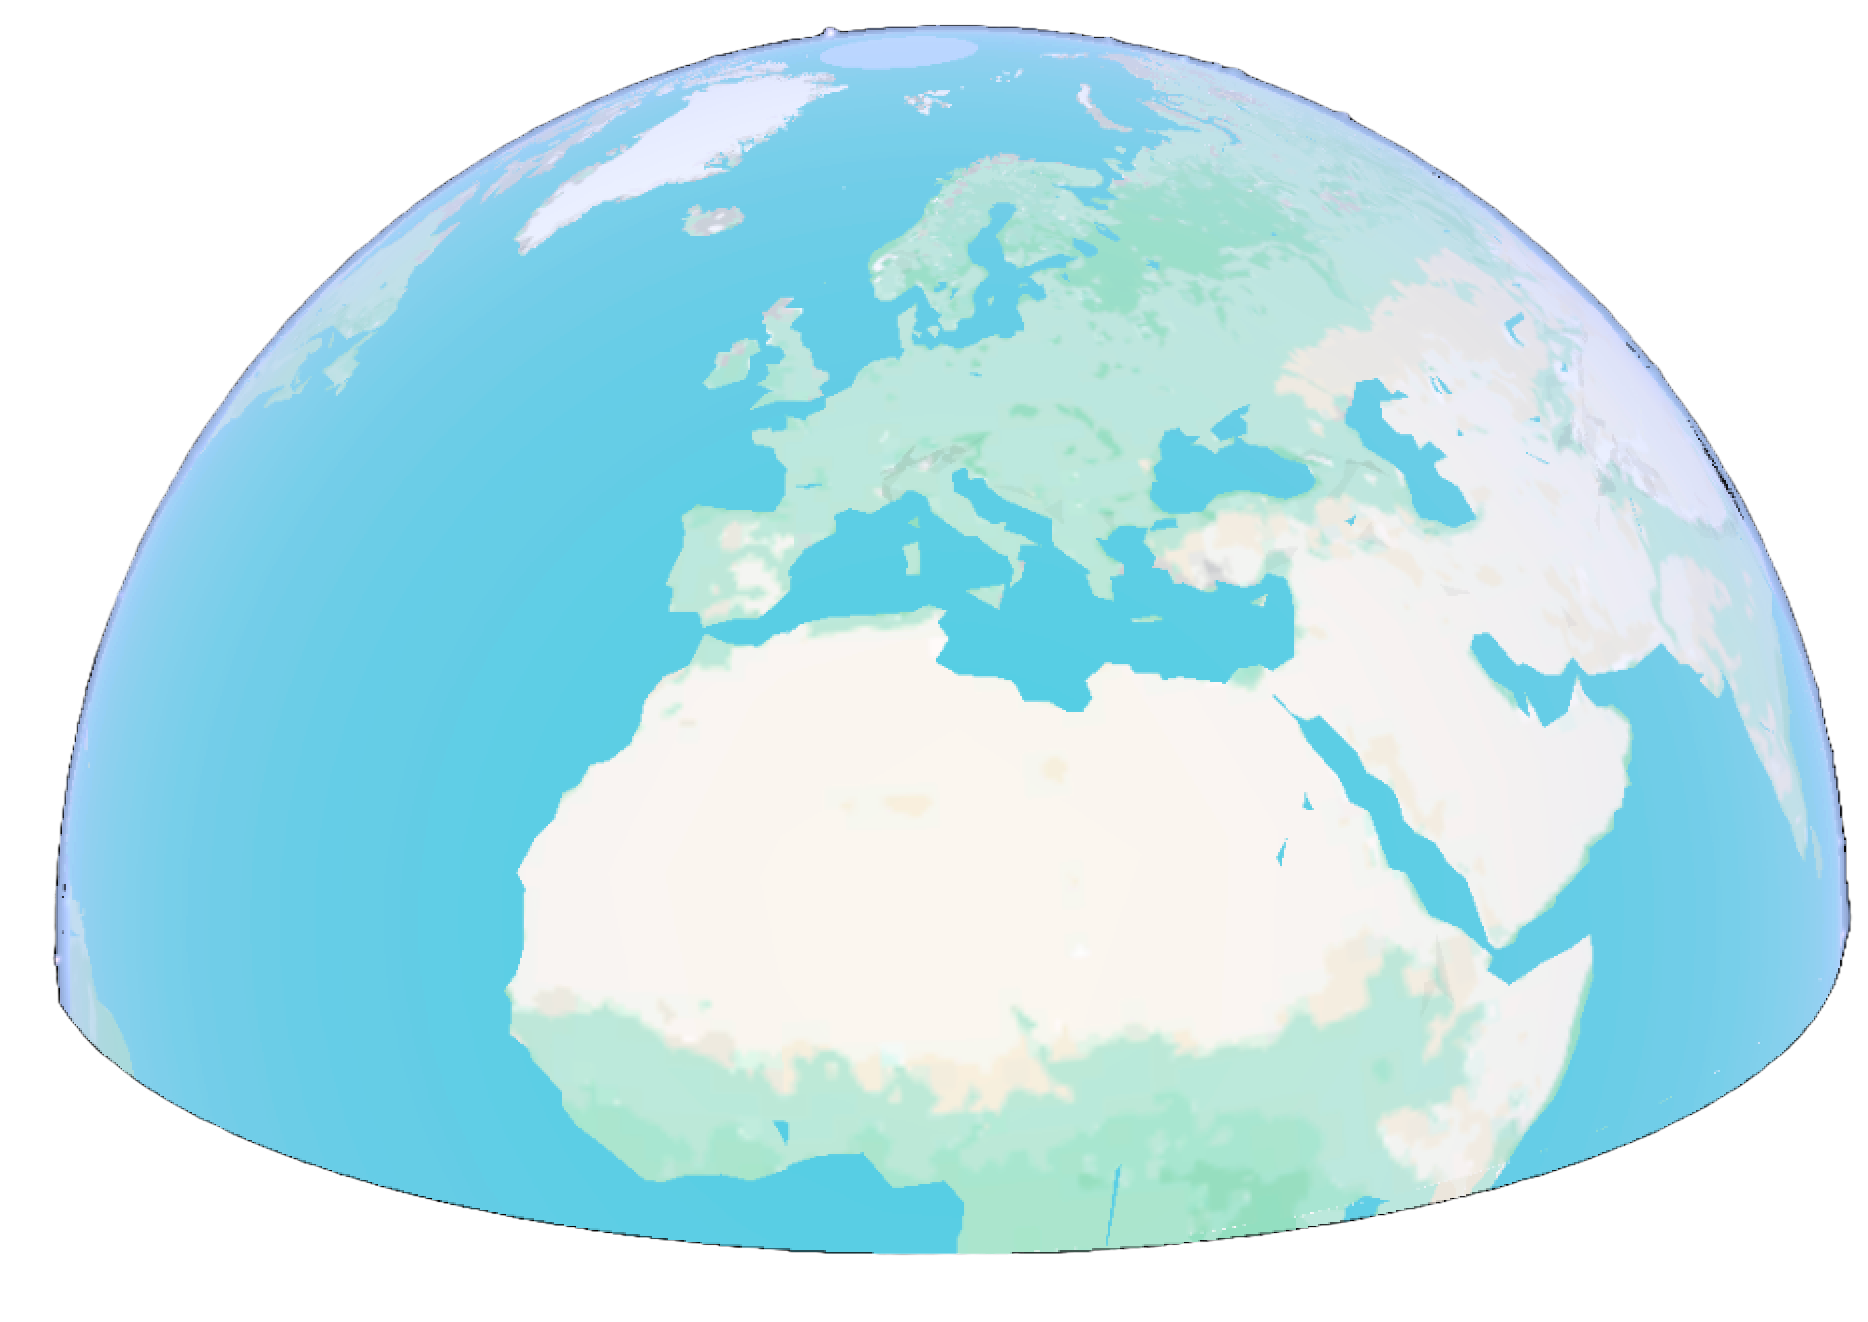
\includegraphics[width=0.5\columnwidth]{../images/hemisphere.png}
        \captionof{figure}{The northern hemisphere obtained by cutting through the equator. Texture: Google Earth}
    \end{center}
    
    An invertible map from the unit-disc to the hemisphere is given by 
    \begin{align*}
        \text{disc-to-hemisphere}(\begin{pmatrix}x & y\end{pmatrix}^\top) = \\\begin{pmatrix}x & y & \sqrt{1 - x^2 - y^2}\end{pmatrix}^\top 
    \end{align*}
    The $x, y$ coordinates span the equatorial plane and the third coordinate is the height of the hemisphere. The inverse of this map corresponds exactly to projecting the hemisphere onto the equatorial plane.
    \begin{center}
        \hspace*{-0.1\columnwidth}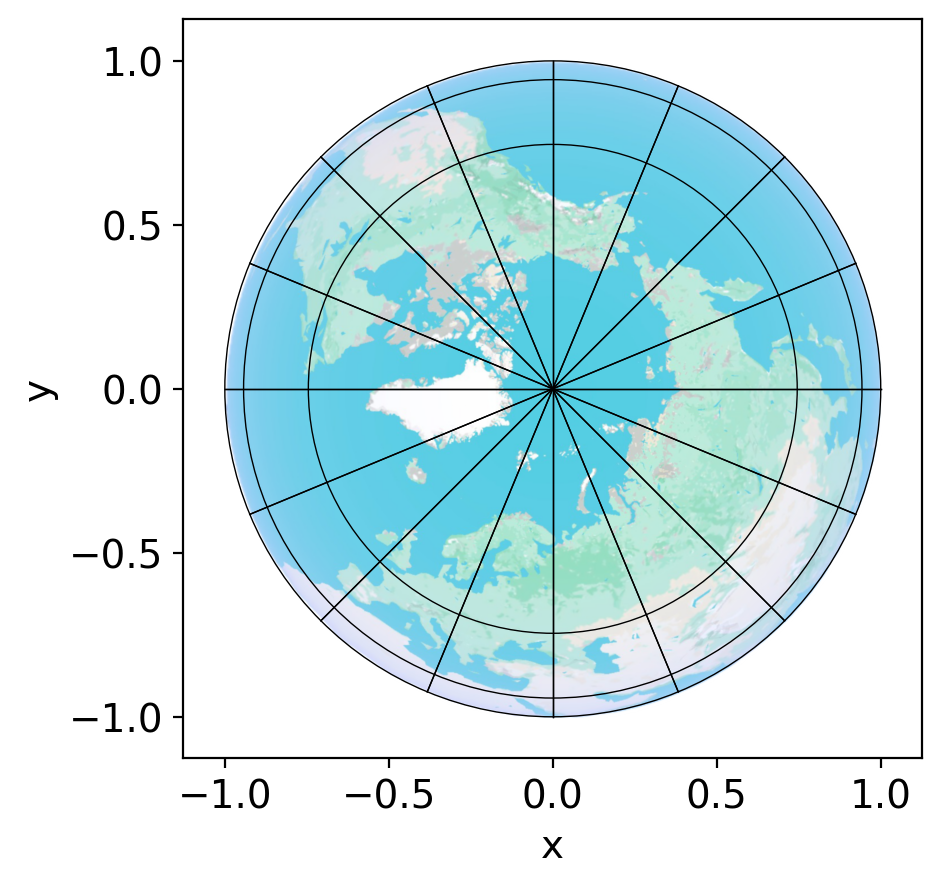
\includegraphics[width=0.7\columnwidth]{../images/hemisphere_circle_of_latitude.png}
        \captionof{figure}{The northern hemisphere projected down onto the equatorial plane. The north pole is placed at local coordinates $(0, 0)$. Three circles of latitude are shown, equally far apart on the hemisphere - note how our map does not render them equally spaced.
        We will further study the properties of this map in a later example.}
    \end{center}
}
    
    
    
\subsection*{Metric Tensor}
Good maps are characterized by being amenable to direct measurements. A weakness of the Equirectangular Projection is the distortion of landmasses at the poles. They are disproportionately big when compared to a countries such as Kenya at the equator. This difference in scale invalidates direct measurements of lengths using a conventional ruler. The Metric Tensor quantifies the distortions induced by the map, and is a vital tool for measurements on coordinate charts.
Before giving a definition, we will further motivate the Metric Tensor by pointing out what one takes for granted in Euclidean space (specifically, $\reals^2$\footnote{$\reals^2$ is technically the set of all ordered pairs of real numbers, but in the context of differential geometry, it is also the Euclidean plane with the Euclidean metric.}). $\reals^2$ is a vector space, meaning that linear combinations of the basis-vectors $e_1$ and $e_2$ are still members of $\reals^2$. In a vector space we can additionally define a norm and an inner product. The Euclidean norm is defined as $||(x,y)||_2 = \sqrt{x^2 + y^2}$ and is used to define the distance $d(\vec{a}, \vec{b}) = ||\vec{a}-\vec{b}||_2$. The Euclidean inner product $\langle \vec{a},\vec{b} \rangle = a_1b_1 +a_2b_2$ relates to the angle $\theta$ (radians) between vectors through $\frac{\langle \vec{a},\vec{b} \rangle}{||\vec{a}||||\vec{b}||} = \cos(\theta)$.
\\
In contrast to $\reals^2$, the surface of the earth is not a vector space. There can be no set of basis vectors, because there is no defined notion of addition or scaling of coordinates, as we do not add or scale pairs ($\text{Lat}^\circ$., $\text{Lon}^\circ$.). And, although we have coordinates, they don't lead to distances or angles, because we don't have the inner product or norm defined. Before diving into the metric tensor, we will have to define the notion of the tangent space.

\definition{Tangent space}{
    The tangent space $\mathcal{TM}_p$ at a point $p$ on a 2-manifold $\mathcal{M}$ is the 2-dimensional real vector space consisting of all tangent vectors to $\mathcal{M}$ at $p$. Each tangent vector can be associated with the velocity of a curve on $\mathcal{M}$ passing through $p$. 
}   
The tangent space is a local "linearization" of the manifold around a point $p$. On the sphere, the tangent space of the north pole is the unique tangent plane that intersects only the north pole. Moving from $p$ along a vector from the tangent space will in general take one away from the manifold.
\definition{Metric Tensor}{
    When using a 2-dimensional coordinate system, the 2D metric tensor is a symmetric, positive-definite 2$\times$2 matrix $g(p) = M \in \reals^{2\times 2}$  where $p$ is a point on the two-dimensional surface specified in local coordinates. $M$ provides a way to measure lengths, angles by describing how the infinitesimal length $ds$ of a change in local coordinates $t=\begin{pmatrix} dx & dy\end{pmatrix}^\top \in \mathcal{TM}_p$ is computed as
    \begin{align*}
        ds^2 &= M_{11}dx^2 + 2M_{12}dxdy + 2M_{22}dy^2 
        \\
        &= \begin{pmatrix} dx & dy\end{pmatrix} \begin{bmatrix} M_{11} & M_{12} \\ M_{12} & M_{22}\end{bmatrix} \begin{pmatrix} dx \\ dy\end{pmatrix} 
        \\
        &= t^\top M\; t
    \end{align*}
    
    and angle $\theta$ between tangent vectors $t, t^\prime \in \mathcal{TM}_p$ are computed as 
    \begin{align}\label{eq:angle}
        \cos(\theta) = \frac{t^\top M \; t}{\sqrt{t^\top M \; t}\sqrt{t^{\prime \top} M \; t^\prime}}
    \end{align}
}
The explicit dependance of the metric tensor $g(p)$ on the coordinate $p$ is often omitted in notation, but we will keep it explicit. 

\definition{Riemannian Metric}{
    A 2D Riemannian metric $g$ maps each local coordinate $p\in C$ to a metric tensor 
    $$g: C\to \reals^{2\times 2}$$
}
To compute gradients and curvature (see later section), the metric must be at least twice differentiable. \\
Informally, $ds$, $dx$, and $dy$ are the same symbol as $dx$ in $\int_0^1 f(x) \;dx$. They are 'differentials'. Intuitively, if we were to relate the integral back to the Riemann sum, $dx$ is the size of the interval in our partition of $[0, 1] \subset \reals$. In the current case, by having $ds$ depend on the position in local coordinates (through the dependence of the metric on $p$), we can assign "bigger partitions" to some areas, which lets us weigh different areas differently. We will use dependence to counteract the non-uniform stretching induced by mappings like Equirectangular projection or our projection of the hemisphere. Positive-definiteness in the definition ensures that all squared infinitesimal distances $ds^2$ will remain positive, no matter the entries in $g$.
\example{Pythagorean Theorem}{
     $g$ can be thought of as encoding a local version of the Pythagorean Theorem. If $g = I_2 = \begin{bmatrix} 1 & 0 \\ 0 & 1\end{bmatrix}$, then the formula for infinitesimal distance reduces to exactly $$ds^2 = dx^2 + dy^2$$ which is similar to $c^2 = a^2 + b^2$. In fact, $I_2$ is the metric tensor of $\reals^2$ independently of position $p$. This reflects the fact that the Pythagorean theorem holds at all positions in $\reals^2$, not just around the origin or some other specific point. If the entries of $g$ change, we will get different identities.
}
\example{Visualizing the Metric Tensor}{
    In cartography, a common way to visualize the degree distortion of the chart is using the Tissot Indicatrix. It shows how a patch of equal area and shape on the earth will be represented on the map. A good approximation of the Tissot Indicatrix can be computed using the metric tensor, by showing (scaled\footnote{The eigenvalues and vectors have been scaled down with a factor of $0.003$ for this figure.}) eigenvectors and -values of the inverse metric tensor as an ellipse, centered at the point of evaluation.
    \begin{center}
        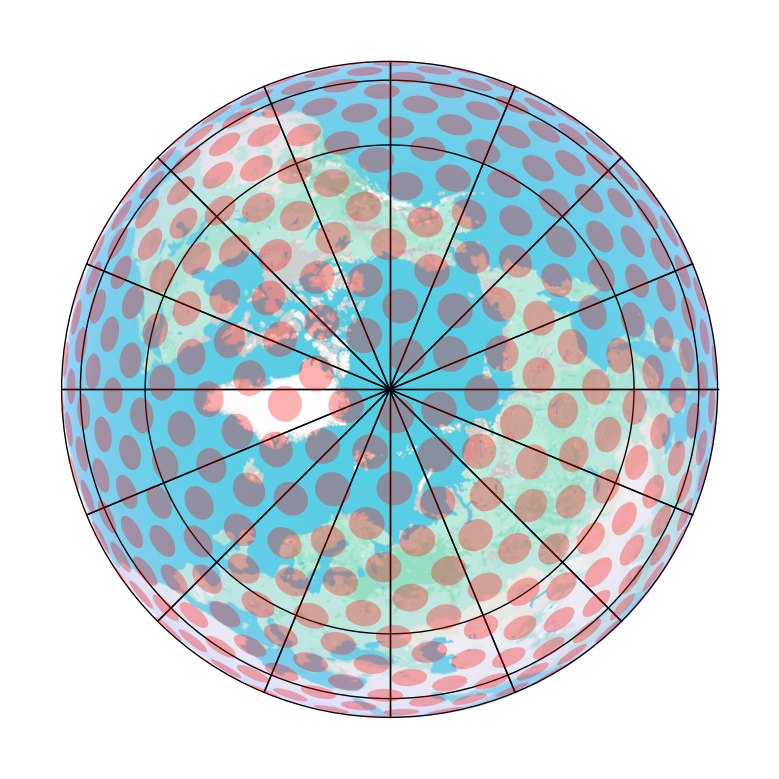
\includegraphics[width=0.95\columnwidth]{../images/hemisphere_tissot_indicatrix.png}
        \captionof{figure}{The hemisphere-map with Tissot Indicatrices at evenly spread locations on the surface of the earth. The radius of the ellipse in a certain direction can be interpreted as the speed at which someone traveling at constant speed on hemisphere would be traveling at when viewed from the map.}
    \end{center}
    Another way visualizing 2D metric tensors are with a pseudo-mesh, which is explored in \cite{mesh_visualization}.
}
\example{Rank of Metric Tensor}{
    The determinant of the 2D Metric Tensor reflects how areas on the surface are scaled locally. By positive-definiteness, the rank of the 2D metric tensor $g(p)$ will always be 2 and the determinant strictly positive. However, positive-semidefinite (rank-deficit) metric tensors can be interesting to study for intuition. 
    
    Consider a metric tensor $\begin{bmatrix} 1 & 0 \\ 0 & 0\end{bmatrix}$, for which the infinitesimal length-formula reduces to $ds = dx$. With this metric, locally the length of infinitesimal $\begin{bmatrix} dx & dy \end{bmatrix}^\top$ depends only on $dx$ with no contribution from $dy$. At this point the space is locally one dimensional, with space being collapsed in direction of the second coordinate basis-vector. 
    For this metric, the $\cos(\theta)$ formula (\ref{eq:angle}) will yield only $0$ and $\pi$, which are the only two possible angles between parallel vectors. 
    
    For a rank 0 matrix (which is the 2x2 zero matrix), $ds = 0$, and angles are undefined as a division by zero occurs.
}


\subsection*{Measuring the length of a path with the Metric Tensor}
If a sailor plans a route (not necessarily straight) on their chart, they will be keen to know the length it represents. From the distortion of the maps seen earlier, we have determined that we cannot simply measure directly, as lengths are not guaranteed to have been represented faithfully. To measure exactly the length of a route, we will have to integrate an expression the infinitesimal length $ds$ of the velocity vector of the line over the whole span of the line. 
\\
We will parameterize the route $r$ with parameter $t \in (0, T)$ to get $r: (0, T) \to \reals^2$. $r$ is in fact a 1-manifold, and the parameterization a choice of local coordinate system. 
\\
Symbolically, the length can be written simply as $L(r) = \int_r ds$ where $ds$ is the infinitesimal length obtained from the metric tensor $g(p)$. But this is not very computable definition. By using the local parameterization we get:

\begin{align} \label{eq:length}
    L(r) = \int_{[0, T]} \sqrt{\nabla r(t)^\top g(r(t))\; \nabla r(t)} \; dt 
\end{align}
\noindent
Even for many seemingly simple cases of $g$ and $r$ this integral has no analytic solution, because it turns out to be an instance of an elliptic integral, which are integrals of the form $\int \sqrt{P(t)}$, where $P$ is some polynomial of $t$. There will be an instance of this in chapter \ref{sec:intrinsic_triangulation}, where we will resort to numerical methods.

\example{Computing the Metric on the chart induced by the 3D hemisphere}{

    The Riemannian metric on the chart induced by the 3D hemisphere can be computed as 
    $$g(p) = J(p)^\top J(p) \in \reals^{2\times 2}$$ 
    where $J(p) \in \reals^{3\times 2}$ is the Jacobian matrix of $\text{disc-to-hemisphere}(\cdot)$ at point $p$, which maps tangent vectors $ \in \reals^2$ to tangents vectors $\in \mathcal{TM} \subset \reals^3$.
    The Jacobian comes out as
    $$ J\left(\begin{pmatrix}x \\ y \end{pmatrix}\right) = \begin{bmatrix}1 & 0 \\ 0 & 1 \\ \frac{-x}{\sqrt{1-x^2-y^2}} & \frac{-y}{\sqrt{1-x^2-y^2}}\end{bmatrix}$$
    which gives the final metric of
    $$g_{\text{hemisphere}}\left(\begin{pmatrix}x \\ y \end{pmatrix}\right)=\frac{1}{1-x^2-y^2} \begin{bmatrix} 1 & xy \\ xy & 1 \end{bmatrix}$$
    This is symmetric, positive definite and well-defined in for $x^2+y^2 < 1$, which is exactly the open unit-disc. At the center, $(0,0)$, the metric tensor coincides with the Euclidean metric, reflecting the fact that the north-pole did not get distorted during the projection, as it was already aligned with the plane we project onto.
}
        

\definition{Riemannian Manifold}{
    A Riemannian Manifold is a pair $\big(\mathcal{M}, g\big)$ of a smooth manifold $\mathcal{M}$ with Riemannian metric $g$.
}
    
\definition{Isometric Immersions and Embeddings, Ambient Space}{
    An isometric immersion of a Riemannian 2-Manifold $\big(\mathcal{M}, g\big)$ into a 2-dimensional submanifold $\hat{\mathcal{M}} \in \reals^3$ is a map $f: \mathcal{M} \to \hat{\mathcal{M}}$ such that the distance between any two points in $\mathcal{M}$ under $g$ is the same as the distance between their images under $f$ measured along the surface of in $\reals^3$. If $f$ is additionally a bijection, meaning that $\hat{\mathcal{M}}$ does not self-intersect, $f$ is an embedding. If it self-intersects it is an immersion. The space that the manifold is mapped into is referred to as the ambient space. Throughout this thesis, where applicable, the ambient space is $\reals^3$.
}
\noindent For our purposes, having an immersion will be sufficient. The embedding is useful for visualization purposes, but is not necessary for the numerical methods we will be using. By construction, $\text{disc-to-hemisphere}(\cdot)$ is an isometric embedding of the Riemannian Manifold given by $$\big(\text{open unit-disc},\; g_{\text{hemisphere}}\big)$$
Another interesting metric we will be working with later is the hyperbolic metric, which is defined on the hyperbolic plane $\mathbb{H}^2$.
\example{The Hyperbolic Metric}{
    The metric of the 2-dimensional hyperbolic plane $\mathbb{H}^2$ is defined as $$g_{\text{hyperbolic}}\left(\begin{pmatrix}
    x \\ y
    \end{pmatrix}\right) = \frac{1}{1- x^2 - y^2} \begin{bmatrix} 1 & 0 \\ 0 & 1\end{bmatrix}$$ with $\begin{bmatrix}
        x & y
        \end{bmatrix}^\top$ as local cartesian coordinates within the unit-disc. The hyperbolic metric is used in the Poincaré disk model of the hyperbolic plane, which, unlike the sphere, is unbounded. It is also not isometrically embeddable in $\reals^3$ (Hilbert's Theorem). Subsets of it can however be embedded. The authors of \cite{shape_from_metric} give a method to embed a portion of the hyperbolic plane in $\reals^3$ and have a great visualization\footnote{For copyright reasons, we will have to make do with the surface of kale leaves, which is a common example of hyperbolic geometry in nature anyway.}. 
    \begin{center}
        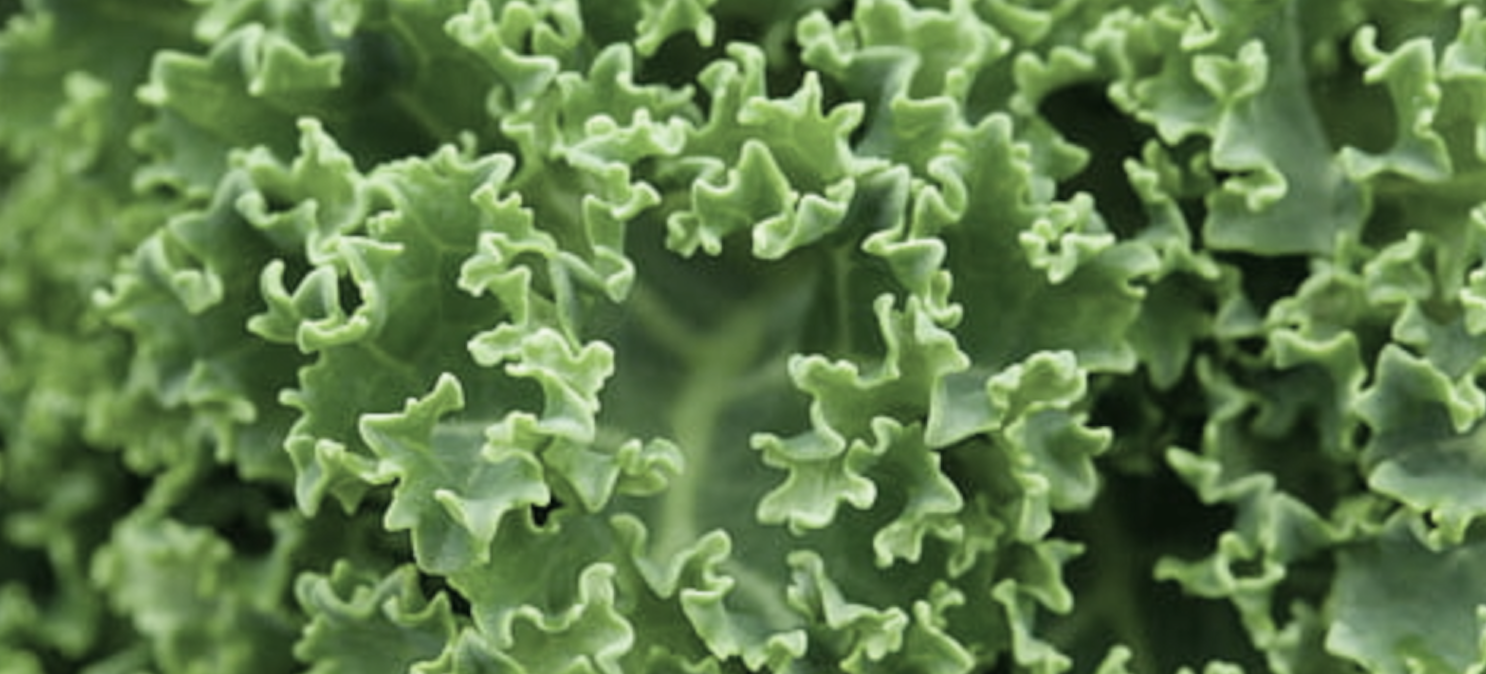
\includegraphics[width=0.95\columnwidth]{../images/hyperbolic_kale.png}
        \captionof{figure}{The surface of kale leaves is hyperbolic. The veins of the leaf are approximately geodesics, which are the shortest paths between points on the leaf. Similarly to how an orange peel cannot be flattened to a sheet without tearing, the kale leaf cannot be flattened to a plane without folding in on itself. One has constant positive gaussian curvature, the other negative.}
        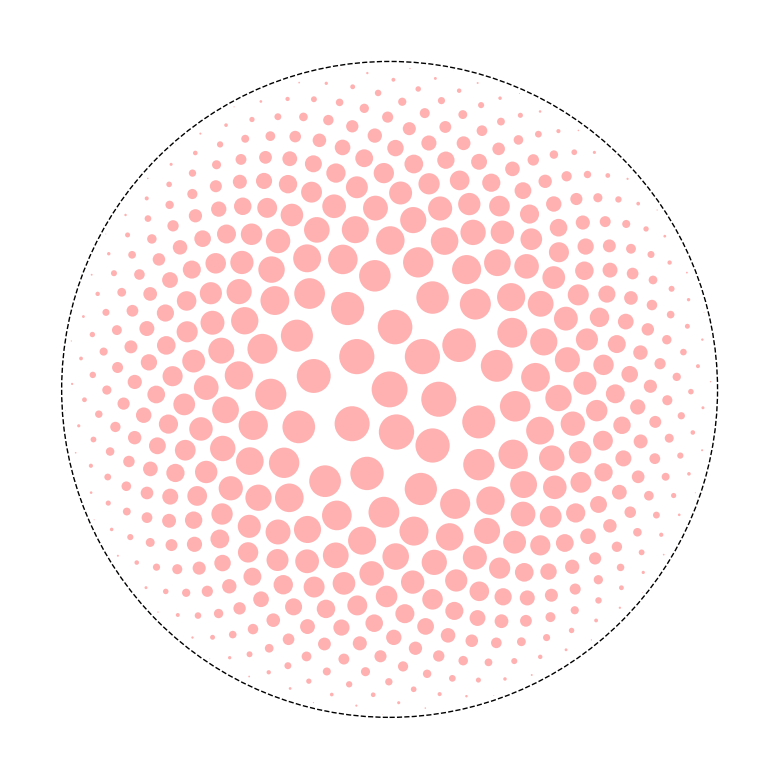
\includegraphics[width=0.8\columnwidth]{../images/hyperbolic_space_tissot.png}
        \captionof{figure}{Tissot Indicatrices shown on Poincaré disc model of the hyperbolic plane. The metric is isotropic, meaning not depending on direction of travel, so the patches are circular. Note that in this figure the indicatrices are \textit{not} uniformly spaced like they were on the hemisphere.}
    \end{center} 
}
\subsubsection*{Boundaries}
Something we have so far been evading is the question of boundaries on a 2-manifold. The boundary of a 2-manifold $\mathcal{M}$ is denoted $\partial \mathcal{M}$ and is a 1-manifold. The boundary of a boundary is always empty. Boundaries are common in the context of numerical solutions of PDEs because of our bounded computational power. If one has an unbounded manifold (say, $\mathcal{M} = \reals^2$ or $\mathbb{H}^2$), one must solve the PDE on a subset of the manifold instead of the whole, which means that a boundary is introduced. However not all manifolds must be truncated like this. The sphere or torus or surfaces of everyday objects are all bounded 2-manifold without a boundary, which means the PDE can usually be solved on the entire domain, and complications with boundaries are avoided.

\subsection*{Intrinsic and Extrinsic Properties}
Properties of Manifolds can be grouped into two categories. Extrinsic properties require the manifold to be viewed as part of the ambient space. The normal vector, which by definition is orthogonal to the tangent space at each point, and position in ambient space are extrinsic properties whose definition require the ambient space. 
\\
Intrinsic properties are independent of any embedding and arise solely from the manifold's internal structure. Lengths of paths and angles of tangent vectors are examples.

\subsection*{Representing Manifolds on a Computer}
We now move to the practical side, anticipating the future involvement of a computer. We will start by introducing the two representations of Riemannian 2-Manifolds of interest: Manifolds given by a local coordinate system and a metric, or Manifolds represented as a triangulation with triangle meshes. Technically, we are representing them as 'Simplicial Complexes', but the term 'triangulation' will be more familiar and simplify the explanation.
\subsection*{Triangulation}
\subsubsection*{Extrinsic Geometry}
A triangle mesh is a collection of vertices $\{V_i\}_{i=0}^{|V|}$ and a set of faces $\{F_i\}_{i=0}^{|F|}$, with $V_i \in \reals^3$ and $F_i \in V \times V \times V$. A face is a an ordered triple of vertices, but even permutations of a face are considered the same face. We say that the face is oriented in one of two ways - this is determines the ambiguity of the normal vector. Edges are defined implicitly by the faces.
A triangle mesh is most commonly represented with each vertex having coordinates in the ambient space. To tie this representation to a specific metric, it is most natural to assume that it represents an isometric immersion (or embedding if the mesh has no self-intersections) of a 2-manifold. [Whats this called? euclidean metric of the ambient space?]. This common representation of a triangulation is called an extrinsic triangulation of the 2-manifold.
\subsubsection*{Intrinsic Geometry}
The extrinsic triangulation allows one to compute edge lengths from the norm of the difference between two adjacent vertices. We can however also make do with an intrinsic triangulation, wherein no reference to the ambient space is made. 
\definition{Intrinsic Triangulation}{
    This representation stores a set of edges $\{E_i\}_{i=0}^{|E|}$ and their lengths $\{e_i\}_{i=0}^{|E|}$. The faces are stored like previously, but defined through an ordered triple of edges instead of vertices. Like faces, edges are an ordered tuple with two possible orientations that must be kept track of. If a face $(E_i, E_j, E_k)$ has associated lengths $(e_i, e_j, e_k)$, there are some restrictions that the lengths must satisfy: 
    $$0 < e_i < e_j + e_k$$
    $$0 < e_j < e_i + e_k$$
    $$0 < e_k < e_i + e_j$$
    This is the strict variant of the triangle inequality, ensuring that all lengths define triangles that can be embedded in $\reals^2$ with non-zero area.
}
\noindent
The advantages of intrinsic triangulations are explored in depth in \cite{sharp2021intrinsic}. The following are useful formulas for computing areas and angles of faces in an intrinsic triangulation.
\example{Heron's Formula for calculating Areas of Faces}{
    Given a face $(E_i, E_j, E_k)$ the area can be computed as 
    \begin{align}
        \text{Area} = \sqrt{s(s-e_i)(s-e_j)(s-e_k)}\label{eq:heron}
    \end{align}
    where $s = \frac{e_i + e_j + e_k}{2}$ is the semiperimeter of the triangle.
}
A good rule of thumb is that if a property cannot be computed from edge-lengths alone, it is not extrinsic \cite{sharp2021intrinsic}. The normal vector or dihedral angles across triangles are examples of these.
\example{The Law of Cosines for calculating Interior Angles of Faces}{
    Given again a face $(E_i, E_j, E_k)$, the cosine of the interior angle $\alpha$ opposite of edge $E_i$ can be computed as 
    $$\cos(\alpha) = \frac{e_j^2 + e_k^2 - e_i^2}{2e_je_k}$$
}
In a subsequent chapter, chapter \ref{sec:intrinsic_triangulation}, we will dive much deeper into intrinsic triangulations, and will give more motivation on why they are useful and when they arise. If confused, think of a triangulation as meaning an extrinsic triangulation for now, which is what is commonly meant when one says "triangle mesh".
\subsubsection*{Manifold Triangle Mesh}
When given an extrinsic triangulation, it is most natural to assume that it represents an isometric immersion (or embedding if the mesh has no self-intersections) of a section of a 2-manifold. Furthermore, for a triangle mesh to represent a 2-manifold, there are some restrictions to how the faces can be connected. An edge must be associated with $n \in \{1, 2\}$ faces and a face cannot share an edge with itself, with the case $n=1$ is realized only at boundary faces. Mesh structures with $n>2$ can be permitted with some tricks that involve "inflating" the mesh (see \cite{nonmanifold_laplacian}), but we will not cover them here and work only with manifold meshes. 
\definition{Dual Mesh}{
    In an extrinsic triangulation, the dual of a triangle mesh is a new mesh ($V^\prime,\; F^\prime$) with 
    $$|V^\prime| = |F| \text{  and  }|F^\prime| = |V|$$
    The vertex $V^\prime_i$ is placed at the center of face $F_i$ of the original mesh, and new faces $F^\prime_i$ are centered at the $V_i$. The two dominant definitions of a triangular center are the barycenter and circumcenter, which lead to the notions of barycentric dual mesh and the circumcentric dual mesh. The barycenter $B_i$ of face $F_i = (V_i, V_j, V_k)$ is simply defined as $B_i = \frac{1}{3}(V_i + V_j + V_k)$, while the circumcenter is the center of the circumcircle, which is the unique circle that passes through all three vertices. 
    \\
    In the dual mesh, two faces that share an edge $E_i$ in the original mesh will become two dual vertices connected by the dual edge $E_i^\prime$.
}
In an intrinsic triangulation, the mapping of vertices to dual faces and faces to dual vertices is the same, but the circumcenter and barycenter cannot be defined explicitly as there are no stored vertex coordinates. One must instead store the length of the dual edge. This length depends on the position of the vertices (barycenter vs circumcenter) and the edge lengths of the original mesh. With intrinsic edge-flips \cite{sharp2021intrinsic}, one can build an intrinsic Delaunay triangulation, which guarantees that the circumcentric dual mesh has positive edge lengths. This leads to high numerical stability and well-conditioned matrices as described in \cite{intrinsic_laplacian}. In this thesis we stick to constructing good triangulations in the first place and will not dive into edge-flips.
\example{Choice of Dual Mesh}{
    The choice of dual will influence edge lengths and dual face areas (see following figures).
    \begin{center}
        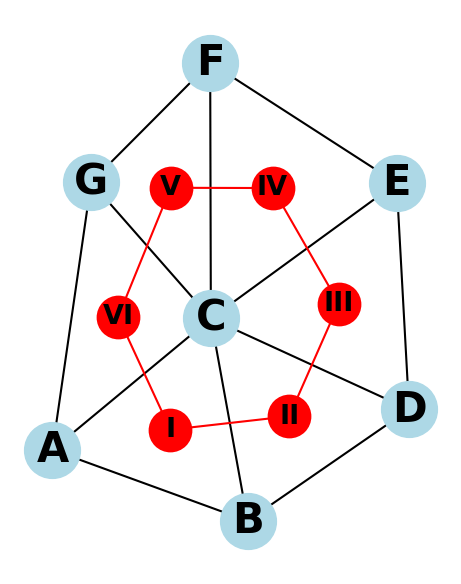
\includegraphics[width=0.7\columnwidth]{../images/barycentric.png}
        \captionof{figure}{Barycentric Dual mesh. The dual vertices in red are placed at the barycenter of each face, guaranteeing a central position and positive edge lengths. 
        For clarity, edges $(I, II)$ and $(B, C)$ are dual, while polygon $(I, II, III, IV, V)$ is dual to vertex $C$.}
        \label{fig:barycentric_dual}
        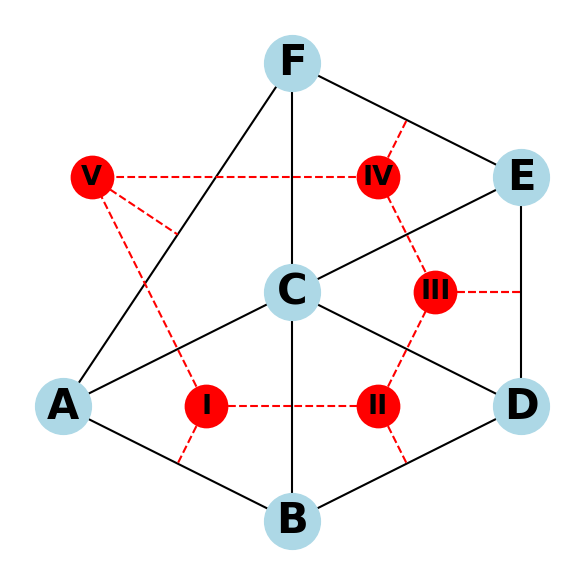
\includegraphics[width=0.7\columnwidth]{../images/circumcentric.png}
        \captionof{figure}{Circumcentric Dual mesh. Each dual vertex is placed at the circumcenter of the face. For obtuse triangles such as $\text{FCA}$, the circumcenter $\text{V}$ lands outside the face. The length of the dual edge is then considered to be negative. The circumcentric dual has the property that pairs of edges and dual edges are orthogonal. Contrast this with the barycentric dual above.}
        \label{fig:circumcentric_dual}
    \end{center}
}

\section*{Building a Laplacian from a Triangle Mesh}
This section will describe how to discretize the differential geometry of manifolds. The goal is to approximate the continuous differential operators on a manifold with discrete operators on a mesh.
\\\\
In 2D Euclidean space, the Laplacian is given by $$\Delta f(x, y) = \frac{d^2}{dx^2}f(x,y) + \frac{d^2}{dy^2}f(x,y)$$ In chapter \ref{sec:pde} we give the discrete version, which has a quite simple form on a rectangular grid. When working in a coordinate space with a metric $g$, the Laplacian cannot be computed directly using the coordinate representation, but must take into account the stretching and deformations induced by the metric. The Laplace-Beltrami operator is the generalization of the Laplacian to Riemannian manifolds.
\definition{Laplace Beltrami Operator}{
    $$\Delta_g f (x) = \frac{\sum_{i=1}^n \!\frac{\partial}{\partial x_i}\!\Big(\!\sqrt{|\text{det}(g(x))|} g(x)^{\!\!-1} \nabla\! f(\!x)\!\Big)}{\sqrt{|\text{det}(g(x))|}}$$
    For notational convenience, we will always refer to the Laplace-Beltrami operator as simply the Laplacian and write $\Delta$, as the domain and metric is clear from context.
}
How one would approximate this quantity from a discrete set of points is not clear. The theory of Discrete Exterior Calculus (DEC) is a powerful tool for this purpose. Although the results we will present are not new, the theory is not widely known and is not covered in standard textbooks on numerical methods and is not part of the standard curriculum in computer science, and so we will spend some time giving a rough overview to motivate the formulas we will use.

\subsection*{Crash Course: Exterior Algebra}
For a more thorough introduction, see \cite{craneDDG}.
Exterior Algebra, also known as Grassmann Algebra, generalizes traditional vectors to $k$-vectors (also called $k$-forms), which form a vector space within each degree $k$. A $0$-vector is identical to a scalar, and a $1$-vector corresponds to a traditional vector in the space.
\\
The binary antisymmetric wedge product $\wedge$ combines an $n$-vector $a$ with a $m$-vector $b$ to form the $(n+m)$-vector $a \wedge b$. Antisymmetry is characterized by $$a \wedge b = -b \wedge a$$
The binary change in sign is related to the two possible orientations of the normal vector of a face or the orientation of an edge. In $n=3$ dimensions, taking the wedge product $v_1 \wedge v_2 = w$ of two $1$-vectors yields a $2$-vector $w$ (a 'bi-vector', something akin to an oriented plane), the magnitude of which is the same as the magnitude of the traditional cross-product of the vectors: $|w| \;= |v_1 \times v_2|$, which is equal with the signed area of their spanned parallelogram. Three vectors can be $\wedge$'ed together to form a $3$-vector, which can be interpreted as an oriented volume. We will however not need to go beyond $2$-vectors when working with 2-manifolds.
\\
The unary 'Hodge star' operator $\star$ maps a $k$-vector to an $(n-k)$-vector. In a sense it maps to a dual representation of the geometric object, as $\star w$ is $1-$vector representing the normal vector of the parallelogram $w$. The notion of duality is strengthed by the relation $\star\star w = w$. For $n=2$, $\star$ maps $0$-vectors to $2$-vectors and vice-versa, while $1$-vectors are mapped to the $1$-vectors that are rotated by $90^\circ$ degrees. The strong connections to the ideas of the dual mesh should be noted. The Exterior Algebra is a language that is well-suited for describing the geometry of manifolds, and is used in the theory of differential forms, which we will cover next.

\subsection*{Crash Course: Exterior Calculus}
For more intuition, see \cite{craneDDG}. For an in-depth coverage relating also to PDEs, see \cite{bryant1991exterior}. In standard multivariable calculus, the differential $ds$ represents an infinitesimal arc length element along a curve. For a 1-dimensional manifold $\mathcal{M}$, the total length can be expressed as $\int_{\mathcal{M}} ds$. Here, $ds$ is derived from the 1-forms $dx$ and $dy$, which serve as basis elements in the local coordinate system. These 1-forms encapsulate how distances are measured in each coordinate direction.

In exterior calculus, we extend the concept of differentials to higher-degree forms by utilizing the previously defined wedge product. The 2-form $dx \wedge dy$ represents an infinitesimal area element. Consequently, the surface area of a 2-dimensional Euclidean patch $R \subset \reals^2$ can be expressed as $\int_{R} dx \wedge dy$. If $R$ is locally parametrized by a 2-dimensional coordinate system, this integral can be evaluated as a nested integral $\int_{y_1}^{y_2}\int_{x_1(y)}^{x_2(y)} dx \; dy$\footnote{This expression should not be surprising, but is mentioned to relate the abstract object $dx \wedge dy$ to something that feels more familiar.}, which computes the area over the specified region.
\\
A function that maps a surface to a continuously varying $k$-form is called a differential $k$-form. The unary exterior derivative operator $\text{d}$ maps a differential $k$-form to a differential $(k+1)$-form. For a differential $0$-form $\phi$ (a scalar field), the exterior derivative $\text{d}\phi$ corresponds to the gradient of $\phi$ in the sense that 
$\text{d}\phi(\mathbf{v}) = \mathbf{v} ^\top \nabla \phi$ for any tangent vector $\mathbf{v}$. This illustrates the close relationship between the exterior derivative and the traditional gradient operator. 
\\
The wedge product $\wedge$ and Hodge star $\star$ treat $k$-vectors and $k$-forms in a symmetric manner. When applied to differential $k$-form, the Hodge star maps it to a differential $(n-k)$-form, where the Hodge-star can be though of being applied elementwise at each point in space. The wedge product can wedge together two differential forms by taking the elementwise wedge product of the two forms for each point in space.
\\
$k$-vectors and $k$-forms are dual\footnote{For an analogy to better get a sense of this symmetry, think of a ruler: the ruler can be used to measure the length of an object (in $\text{cm}$), but the object can also be used to measure the length of the ruler (in object-length-units)} in the sense that a $1$-vector $v$ can be related to a $1$-form $\nu$ through the unary musical operators $\flat$ ("flat") and $\sharp$ ("sharp"), $$v^\flat = \nu \iff v = \nu^\sharp$$
Unlike the gradient, which is limited to scalar fields, the exterior derivative provides a building block for various differential operators, such as curl ($\text{curl}\;F =\star \text{d}F^\flat$) and divergence ($\text{div}\;F =\star \text{d}\star F^\flat$). Intuitively, the idea that the curl and divergence are related by the Hodge star should seem sensible, as these are in a sense orthogonal measures. \\ We have finally arrived to a formula for the Laplace-Beltrami operator, which is the main focus of this entire chapter. 
\definition{Laplace-Beltrami Operator, Exterior Calculus Form}{
    The Laplacian of a scalar-valued\footnote{This can also be generalized to $k$-vector-valued functions $g$, for which the Laplacian takes the form $\Delta g = \star \text{d}\!\star\!\text{d}g + \text{d}\!\star\!\text{d}\!\star\! g$. We will not dig deeper here.} function $f$ is defined as
    $$\Delta f = \star \text{d}\!\star\!\text{d}f$$
    which is again a scalar function. As in the Euclidean definition, the Laplacian can also be expressed as the divergence of the gradient, $$\Delta f = \text{div} \nabla f$$ exressing the divergence with $\star \text{d}\star$ and the gradient operator with $\text{d}$.
}\noindent
The notation hides a lot of complexity and changes in objects (as good notation should). For newcomers, it is instructive to take a look under the hood to convince oneself that what is going is sensible in terms of input/output.
\example{Investigating the form of the Laplacian}{
    We will unpack the definition of the Laplacian of $f$, $\star \text{d}\!\star\!\text{d}f$. We start with
    $f$, a scalar-function, or, equivalently, a differential $0$-form. $\text{d}f$ takes our differential $0$-form to a differential $1$-form. For ambient space dimension $n$, $\star\text{d}f$ then maps this to a dual representation as a differential $(n-1)$-form, and another application of the exterior derivative then gives $\text{d}\star\text{d}f$, which has again increased the degree to a differential $n$-form. A final application of $\star$ then takes us to the dual representation, resulting in a differential $(n-n)$-form, a $0$-form, back to a scalar field, as one would expect from the Laplacian.
    Note that the choice of the ambient space dimension $n$ did not matter, as it was cancelled out in the end. The Laplacian is a scalar field, no matter the dimension of the ambient space, which emphasizes the intrinsic nature of it.
}
This formula for the Laplacian does not seem like it has brought us any closer to a discrete representation of the Laplacian. However, the exterior derivative $\text{d}$ and Hodge star $\star$ operators can be discretized in a way that is consistent with the geometry of the mesh. This is the main result of Discrete Exterior Calculus, which we will now introduce.
\subsection*{Crash Course: Discrete Exterior Calculus}
Discrete Exterior Calculus (DEC) is a relatively new (2003, \cite{discrete_exterior_calculus_thesis}, \cite{discrete_exterior_calculus}) theory that fully embraces the discrete nature of triangle meshes. It is a discrete version of the exterior calculus, with corresponding discrete versions of the Hodge star and exterior derivative, all of which are directly applicable to manifold triangle meshes. We will give the main resuls relevant to the probabilistic numerical solver on manifolds, which are the interpretation of the mesh as a manifold and how to build the Laplacian matrix. 
\\
In DEC, one uses the “exact input” hypothesis \cite{sharp2021intrinsic}, which states that the mesh is not interpreted as an approximation of a manifold, but represents the manifold itself. The mesh forms a partition of the manifold into faces, and each triangular face is assumed to be an isometric embedding of a triangular patch of the manifold. The mesh in its entirety then consists of many patches, each of which are endowed with a local Euclidean metric. A local coordinate system per face can be defined using barycentric\footnote{Barycentric coordinates are local coordinates for simplices. A point, straight line, triangle, and tetrahedron are instances of a $0$-, $1$-, $2$-, and $3$-simplices respectively. For $|V|$ vertices $(v_1, \dots, v_{|V|})\in \reals^{n \times |V|}$ in some $k \geq |V|$-dimensional ambient space, local coordinates $\Lambda = (\lambda_1, \dots, \lambda_{|V|}) \geq 0$ with $\sum_{i=1}^{|V|} \lambda_i = 1$ correspond to point $p(\Lambda) = \sum_{i=1}^{|V|} \lambda_i v_i$ which is a convex combination of the vertices, parametrizing the interior and boundary.} coordinates. The length $e_a$ of an edge $(V_i, V_j)$ between two vertices will thus represent the actual length of the path along the manifold between the two vertices.

\example{Discretizing differential $0$- and $1$-forms onto a Manifold Triangle Mesh}{
    Scalar fields (differential 0-forms) on the manifold can discretized onto the mesh by sampling the scalar value of $\alpha(V_i)$ at each vertex $V_i$. A discretized scalar function is then stored as a $|V|$-dimensional vector $\bar{\alpha}_i = \alpha(V_i)$. 
    \\
    To represent a discrete differential $1$-form $\beta$ on the manifold, an edge $(V_a, V_b)$ is mapped to a parameterized paths 
    $$r_i(t)\footnote{This linear combination is permitted because we know the straight line (in ambient space coordinates) between two neighboring vertices is the edge, a linear subspace of the manifold triangle mesh.}=(1-t)V_a + tV_b \in \mathcal{M}$$
    The discretized differential 1-form along all edges $E_i$ becomes then a vector $\bar{\beta} \in \reals^{|E|}$  with
    \begin{align*}
        \bar{\beta}_i &= \int_{[0,1]} \frac{dr_i}{dt}(t)^\top \beta(r_i(t)) \; dt
        \\
        &=\int_{[0,1]} (V_b - V_a)^\top \beta(r_i(t)) \; dt
    \end{align*}
    The orientation of the edge determines the sign of $\bar{\beta}_i$ and is therefore necessary to keep track of. $\bar{\beta}_i$ can be interpreted as a degree of "alignment" between the vector field and the edge.
    \\
    For intuition, differential $0$-forms (scalar functions) are sampled onto the $0$-dimensional components of the mesh, the vertices. Differential $1$-forms ("vector fields") are sampled onto the $1$-dimensional components, the edges. Even differential $2$-forms (bivector fields) can be sampled onto the $2$-dimensional components, the faces. The three are therefore stored, respectively, as real vectors of length $|V|$, $|E|$, and $|F|$.
}
The discrete exterior calculus analog of the Laplacian is the DEC Laplacian $L$, also known as the cotan-Laplacian
\definition{DEC Laplacian / cotan-Laplacian}{
    In DEC, each of the operators $\star \text{d}\!\star\!\text{d}$ become a matrix, and so the discrete Laplacian is a matrix as well. Specifically, the equation turns into
    $$L = \star_0^{-1} \text{d}_1\!\star_1\!\text{d}_0 \in \reals^{|V|\times |V|}$$
    where $\star_0^{-1}$ is simply the matrix inverse of $\star_0$. This formula is by \cite{intrinsic_laplacian} for 2-manifolds, but can also be derived through a variational formulation as in the finite element method. Formulas exist also for $n-$dimensional manifolds \cite{ndcotangent}. $L$ has the property that each row-sum is zero, which means that constant functions (vectors with the same entry everywhere) are in the nullspace of $L$, just like the continuous variant.
    % The name stems from the fact that it can be built explicitly as a sum of cotangent weights in a neighborhood of each vertex,
    % \begin{align*}
    %     w_{ij} &= \sum_{ijk \in F} \frac{1}{2}\cot(\theta_{ij})
    % \end{align*}
    % $w_{ij}$ is the cotangent weight, weighted over all triangles in which an edge $ij$ appears, with $\theta_{ij}$ as the angle of the triangle opposite the edge $ij$.
    % The cotan-Laplacian is then built as 
    % \begin{align*}
    %     L_{ij} &= \begin{cases}
    %         -w_{ij} & \text{if } i \neq j
    %         \\
    %         \sum_{k \in N(i)} w_{ik} & \text{if } i = j
    %     \end{cases}
    % \end{align*}
    % with $N(i)$ as the set of all vertices connected to $i$ by an edge.
}
The four terms in the definition of the DEC Laplacian will be covered next.
\definition{$\text{d}_0$}{
    The discrete exterior derivative $\text{d}_0 \in \{-1, 0, 1\}^{|E|\times |V|}$ is a matrix that takes a discrete differential $0$-form to a discrete differential $1$-form. This is akin to how the standard exterior derivative increases the degree of a differential form. The value of the $1$-form at edge is the difference of the values at the two vertices, where the sign depends on the orientation of the edge
    $${\text{d}_0}_{ij} = \mathbf{1}[E_i = (V_j \to \cdot)] - \mathbf{1}[E_i = (\cdot \to V_j)]$$
    Each entry is in $\{-1, 0, 1\}$. Because an edge has only two endpoints, a row in $\text{d}_0$ will have at most two non-zero entries of opposing sign. Each column will have nonzero entries, equal to the number of edges incident to vertex $i$.
}
If $\text{d}_0$ is left-multiplied onto a discrete scalar function defined on the vertices, the result is a vector field represented on the edges. This is the discrete analog of the gradient operator. It can be thought of a generalization of the classic finite-differences formulas in Euclidean spaces. 
\definition{$\star_1$}{
    The Hodge-star from $1$-forms in $(n\!\!=\!\!2)$-dimensional space $\reals^2$ is a matrix $\star_1 \in \reals^{|E|\times |E|}$ that takes a discretized vector field $\bar{\phi} \in \reals^{|E|}$ defined over the edges and returns a discretized vector field over the edges of the dual mesh. $\star_1\bar{\phi}$ represents the discretization of the dual vector field. The matrix is a diagonal matrix that holds on each entry $${\star_1}_{ii} = \frac{e_i^\prime}{e_i}$$ with $e_i^\prime$ as the length of the dual edge. $\star_1\bar{\phi}$ can be interpreted as a vector field that flows everywhere orthogonally to the original vector field (rotated $90^\circ$ everywhere).
}
Constructing $\star_1$ is the most computationally expensive part of building the Laplacian, as it requires the computation of the dual edge lengths. These and other related quantities can however all be precomputed and stored efficiently in sparse matrix structures for later use.
\example{Calculating the Circumcentric Dual Edge Lengths}{
    In extrinsic geometry with vertex coordinates given in ambient space, the circumcentric dual mesh can be constructed explicitly, from which the dual edge lengths can be easily computed. In intrinsic geometry however, we can use the cotangent weights to compute the dual edge lengths.\\
    Assume vertices $A, B, C, D$ with triangles $ABC$, $BCD$ with shared edge $BC$ with length $e = |BC|$. The dual edge length $e^\prime$ is the distance between the two circumenters of the neighboring triangles. We can decompose this into the sum of the distance from edge $BC$ to each circumcenter.
    The circumradius $R$ can be calculated as (\cite{sharp2021intrinsic}) 
    $$R = \frac{|AB||BC||CA|}{4\Delta} = \frac{|AB|}{2\sin{\theta}}$$
    with $\Delta$ the area of the triangle (given by Heron's formula (\ref{eq:heron})). The second equality is an alternative expression by the law of sines with $\theta = \angle CAB$. The distance to the segment $AB$
    $$R\cos(\theta) = \frac{|BC|}{2}\frac{\cos{\theta}}{\sin{\theta}} = \frac{|BC|}{2}\cot{\theta}$$
    In a symmetric manner we calculate the distance from $BC$ to the circumcenter of $BCD$ as $\frac{|AB|}{2}\cot{\gamma}$ for opposing angle $\gamma = \angle CDB$, yielding final dual edge length $$e^\prime = \frac{|AB|}{2}(\cot{\theta} + \cot{\gamma})$$
    Finally, this results in $${\star_1}_{ii} = \frac{e_i^\prime}{e_i} = \frac{1}{2}(\cot{\theta} + \cot{\gamma})$$ for appropriate values of $\theta$ and $\gamma$ related to edge at index $i$. At a boundary edge, one of the terms in the sum will be defined as zero. \\This formula is what gives rise to the name "cotan-Laplacian".
}
With the dual edges in place, we now move to the final two matrices in the DEC Laplacian.
\definition{$\text{d}_1$}{
    The exterior derivative matrix $\text{d}_1 \in \{-1, 0, 1\}^{|F|\times |E|}$ is a matrix that takes a discretized differential 1-form on edges and maps it to a discrete differential 2-form on faces. Similarly to $\text{d}_0$, the value of the $2$-form at face $F_i$ is sum of the values at the edges that make up the face, with the sign depending on the orientation of the face.
    \begin{align*}
        {\text{d}_1}_{ij} &= \mathbf{1}[E_j = (V_a \to V_b) \in F_i = (V_a, V_b, V_c)] 
        \\&- \mathbf{1}[E_j = (V_b \to V_a) \in F_i = (V_a, V_b, V_c)]
    \end{align*}
    Keep in mind that even permutations of a face are considered the same face, so $(V_a, V_b, V_c) = (V_c, V_a, V_b) = (V_b, V_c, V_a)$. Rows in $\text{d}_1$ are related to faces and will have three non-zero entries in $\{-1, 0, 1\}$, and each column, related to an edge, will have one or two non-zero entries (one if it is a boundary edge).
}
\definition{$\star_0$}{
    The Hodge-star from $0$-forms in $(n\!\!=\!\!2)$-dimensional space $\reals^2$ is a matrix $\star_0 \in \reals_+^{|F|\times |V|}$ that takes a discretized differential $0$-form and returns a discretized $2$-form over the faces of the dual mesh. The matrix is a diagonal matrix that holds in each entry $${\star_0}_{ii} = A_i$$ with $A_i$ the area of the associated dual face of the vertex $i$. In the DEC Laplacian, $\star_0$ is inverted, but since the matrix is diagonal, this is a simple operation.
}
\example{Dual Face Areas}{
    The discrete Hodge-star is still an open question and a topic of research (\cite{hodge}). While the discrete exterior derivative is in a sense $\textit{exact}$ on the manifold (\cite{craneDDG}), the discrete Hodge-stars $\star_0$, $\star_1$ are only an approximation, which stems from the ambiguity of the two possible choices of a dual mesh. 
    \\
    The barycentric dual area of a vertex is simply $\frac{1}{3}$ the sum of the areas of the adjacent triangles, while the circumcentric dual takes a bit more work. However, in practice (\cite{discrete_exterior_calculus}) on a Delaunay triangulation, the circumcentric dual area is well approximated by the barycentric dual area, and so this is also the method used in this thesis.
}
With all the preceding definitions in place, the DEC Laplacian can now be obtained as the matrix $L \in \reals^{|V| \times |V|} $ and can be used as a drop-in replacement for finite-difference schemes.

\subsection*{Bringing it together: Computing the Discrete Laplacian of a Simple Mesh}
\begin{figure}[h]
    \centering
    \hspace*{-5mm}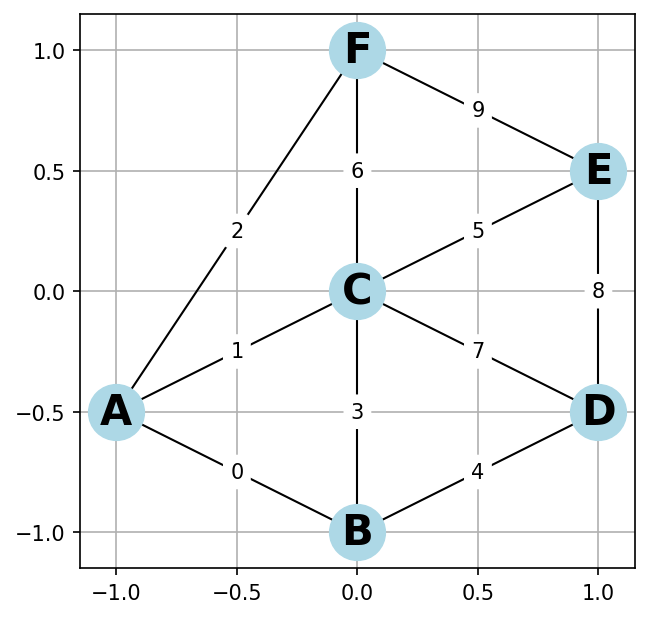
\includegraphics[width=0.9\columnwidth]{../images/dec_example_mesh.png}
    \caption{The mesh we will be working with. Edge index is labeled on the edge}
    \label{fig:dec_initial_mesh}
\end{figure}\noindent
In this example, we work with the small manifold mesh in fig \ref{fig:dec_initial_mesh}. It is planar, but this is just for convenience of visualization. We have a total of $6$ vertices and $10$ edges. The vertices are ordered alphabetically as $V$ = $(A, B, C, D, E, F)$. We choose to both direct and order edges alphabetically, so that we have $E$ = $\Big((A \to B)$, $(A \to C)$, $(A \to F)$ $(B \to D)$, $(C \to D)$, $\dots$, $(E \to F)\Big)$. The order is not important, as long as it is consistent.
\\
\\
$\text{d}_0  \in \{-1, 0, 1\}^{10 \times 6}$ is computed by the formula given earlier, and the result is
$$\text{d}_0 = \left[\begin{array}{rrrrrr}
    \!\!-1 &  1 &  0 &  0 &  0 &  0
    \\\!\!-1 &  0 &  1 &  0 &  0 &  0
    \\\!\!-1 &  0 &  0 &  0 &  0 &  1
    \\ 0 & \!\!-1 &  1 &  0 &  0 &  0
    \\ 0 & \!\!-1 &  0 &  1 &  0 &  0
    \\ 0 &  0 & \!\!-1 &  1 &  0 &  0
    \\ 0 &  0 & \!\!-1 &  0 &  1 &  0
    \\ 0 &  0 & \!\!-1 &  0 &  0 &  1
    \\ 0 &  0 &  0 & \!\!-1 &  1 &  0
    \\ 0 &  0 &  0 &  0 & \!\!-1 &  1
\end{array}\right]$$
\\ $\text{d}_1 \in \{-1, 0, 1\}^{5 \times 10}$ is computed by the formula given earlier, and the result is
$$\text{d}_1 = \left[\begin{array}{rrrrrrrrrr}
1 & \!\!\!-1 &  0 &  1 &  0 &  0 &  0 &  0 &  0 &  0
\\ 0 &  0 &  0 &  1 & \!\!\!-1 &  1 &  0 &  0 &  0 &  0
\\ 0 &  0 &  0 &  0 &  0 &  1 & \!\!\!-1 &  0 &  1 &  0
\\ 0 &  0 &  0 &  0 &  0 &  0 &  1 & \!\!\!-1 &  0 &  1
\\ 0 &  1 & \!\!\!-1 &  0 &  0 &  0 &  0 &  1 &  0 &  0
\end{array}\right]$$
Both $\text{d}_0$ and $\text{d}_1$ depend only on the topology of the mesh. For $\star_0$ and $\star_1$, we will need to consider the actual edge lengths and face areas.
The dual areas turn out to be 
$$\star_0 = \text{diag} (\begin{pmatrix}
    2/6 & 2/6 & 5/6 & 2/6 & 2/6 & 2/6 \end{pmatrix}^\top)$$
while the ratio of the dual edge to the primal edge length is $\star_1$,
$$\star_1 = \text{diag} (\frac{1}{8}\begin{pmatrix}
   2 & 8 & -2 & 6 & 2 & 4 & 4 & 10 & 3 & 2 \end{pmatrix}^\top)$$
The negative entry for edge 2 is due to the circumcentric dual, see figure $\ref{fig:circumcentric_dual}$. With the aforementioned edge-flips \cite{sharp2021intrinsic}, the mesh can be locally rewired in a way that will ensure that all dual edge lengths are positive.
\\
Finally, multiplying these matrices together yields the Laplacian matrix $L = \star_0^{-1} \text{d}_1\star_1\text{d}_0 = $
$$\left[\!\!\begin{array}{rrrrrr}
     3   & -0.75 & -3   &  0  &  0  &  0.75 
    \\-0.75 &  3.75 & -2.25 & -0.75 &  0  &  0  
    \\-1.2  & -0.9  &  4.8  & -0.6  & -0.6  & -1.5  
    \\ 0  & -0.75 & -1.5  &  3.375& -1.125&  0  
    \\ 0  &  0  & -1.5  & -1.125&  3.375& -0.75 
    \\ 0.75 &  0  & -3.75 &  0  & -0.75 &  3.75 
\end{array}\!\!\right]$$
$L$ can be used immediately as a drop-in replacement of the Laplace-operator $\Delta$ in the Method of Lines mentioned in chapter \ref{sec:pde} which this is exactly how we will use it in the later chapters. One can encoding Neumann boundary conditions which is covered in high detail in \cite{craneDDG} - in our experiments, we will stick to the simpler Dirichlet boundary conditions.
\ifdefined\COMPILINGFROMMAIN
\else    
    \end{document}
\fi

\clearpage
\section{Building an Intrinsic Triangulation from a Metric}\label{sec:intrinsic_triangulation}
\ifdefined\COMPILINGFROMMAIN
\else
    %%%%HEADER
\documentclass[twocolumn]{article}
\usepackage[a4paper, margin=1in, columnsep=20pt]{geometry}
\usepackage{amsmath, amssymb, graphicx, hyperref}
\usepackage[most,skins,breakable]{tcolorbox}
\usepackage[symbol]{footmisc}
\usetikzlibrary{calc}
\usepackage{xcolor}
\usepackage{caption}
\usepackage{algorithm}
\usepackage{algpseudocodex}
\usepackage{tikz}
\usepackage{listings}
\usetikzlibrary{arrows.meta, positioning}
\tcbuselibrary{listingsutf8}
\usepackage{microtype}
\usepackage{blindtext}
\usepackage{bookmark}
\usepackage{breqn}
\usepackage[backend=biber,style=numeric]{biblatex} % 
\addbibresource{../references.bib}

% Define style for the listings environment
\lstdefinestyle{mystyle}{
    basicstyle=\ttfamily\small,
    breaklines=true,
    escapeinside={(*@}{@*)}, % Allows math mode within listings
    numbers=left,
    numberstyle=\tiny,
    frame=single,
    keywordstyle=\color{blue}\bfseries,
    commentstyle=\color{green!50!black},
    stringstyle=\color{red}
}


\def\reals{\mathbb{R}}
% Define the custom definition box and command
\newtcolorbox{mydefinition}[2][]{%
    text width=0.95\columnwidth,
    before=\vspace{1mm}, 
    after=\vspace{1mm}, 
    colback=gray!10, % Background color (light gray)
    colframe=black!70,  % Border color
    coltitle=gray!10,  % Title color
    fonttitle=\bfseries, % Title font style
    sharp corners,   % Box style
    left=2pt,
    breakable,
    right=2pt,
    top=2pt,
    bottom=2pt,
    enhanced jigsaw,
    title=Definition: {#1},         % Title passed as the first argument
    colupper=black,  % Ensure proper content handling
    pad at break*=1pc,
    overlay first and middle={
        \coordinate (A1) at ($(interior.south east) + (-10pt,5pt)$);
        \coordinate (C1) at ($(interior.south east) + (-6pt,7.5pt)$);
        \draw[fill=black!50] (A1) -- +(0,5pt) -- (C1) -- cycle;
    }
    }
    
\newcommand{\definition}[2]{%
    \noindent%
    \begin{mydefinition}[#1]%
        .#2%
    \end{mydefinition}%
    \noindent
}

\newtcolorbox{myexample}[2][]{%
    text width=0.95\columnwidth,
    before=\vspace{1mm}, 
    after=\vspace{1mm}, 
    colback=orange!3, % Background color (light gray)
    colframe=black!70,  % Border color
    coltitle=gray!10,  % Title color
    fonttitle=\bfseries, % Title font style
    sharp corners,   % Box style
    left=2pt,
    right=2pt,
    top=2pt,
    bottom=2pt,
    breakable,
    title=Intuition: {#1},         % Title passed as the first argument
    pad at break*=1pc,
    overlay first and middle={
        \coordinate (A1) at ($(interior.south east) + (-10pt,5pt)$);
        \coordinate (C1) at ($(interior.south east) + (-6pt,7.5pt)$);
        \draw[fill=black!50] (A1) -- +(0,5pt) -- (C1) -- cycle;
    }
}

\newcommand{\example}[2]{%
    \noindent%
    \begin{myexample}[#1]%
    .#2%
    \end{myexample}%
    \noindent
}

\newtcolorbox{algobox}[2][]{%
    text width=0.95\columnwidth,
    before=\vspace{1mm}, 
    after=\vspace{1mm}, 
    colback=blue!5, % Background color (light gray)
    colframe=black!70,  % Border color
    coltitle=gray!10,  % Title color
    fonttitle=\bfseries, % Title font style
    sharp corners,   % Box style
    left=2pt,
    right=2pt,
    top=2pt,
    bottom=2pt,
    breakable,
    title=Algorithm: {#1},         % Title passed as the first argument
    pad at break*=1pc,
    overlay first and middle={
        \coordinate (A1) at ($(interior.south east) + (-10pt,5pt)$);
        \coordinate (C1) at ($(interior.south east) + (-6pt,7.5pt)$);
        \draw[fill=black!50] (A1) -- +(0,5pt) -- (C1) -- cycle;
    }
}

\newcommand{\algorithmbox}[2]{%
\noindent%
    \begin{algobox}[#1]%
    .#2%
    \end{algobox}%
    \noindent
}
%%%%HEADER

    \begin{document}
\fi
We will now describe a way to build an intrinsic triangulation of a Riemannian 2-Manifold $\big(\mathcal{M}, g\big)$, which enables the use of tools from Discrete Exterior Calculus, the cotan-Laplacian in which we are most interested in here. An intrinsic triangulation represents the intrinsic geometry - not an embedding of $\mathcal{M}$ into some ambient space. This is emphasized by the fact that we will be working with vertex coordinates in 2 dimensions, and will be interested in the edge-lengths under $g$, not the Euclidean distances between the vertices.
\\
\subsection*{Computing Edge Lengths through the Coordinate Space} 
Let the metric $g : C \to \reals^{2\times2}$. We will be triangulating the local-coordinate domain $C\subset \reals^2$ of the metric $g$, but using $g$ to measure the properties (lengths, areas) of the triangles. The triangulation will be an intrinsic triangulation of the manifold by encoding the metric in the edges and by having no reference to the ambient space.
\\
In the introduction we have given the general formula for computing lengths of paths under the metric $g$. We will here consider the edges of the mesh as paths, and compute their length using this same formula. 
\\
For an edge $E = (A, B)$, we will parametrize it as $$r_i(t) = (1-t)A + tB$$ for $t\in[0,1]$. The measured length along the edge from $A$ to $B$, $e_i = m(A, B)$ is then computed as
\begin{align*}
    m(A, B) &:= \int_{0}^{1}\! \sqrt{\nabla r_i(t)^\top g(r_i(t)) \nabla r_i(t)} \, dt
    \\ 
    &= \int_{0}^{1}\! \sqrt{(B\!-\!A)^\top g(r_i(t)) (B\!-\!A)} \, dt
\end{align*}
By abbreviating the integrand as $$f(t) = \sqrt{(B\!-\!A)^\top g(r_i(t)) (B\!-\!A)}$$ we can get a simple formula for a numerical approximation using the trapezoidal rule:
\begin{align*}
    m(A, B) &= \int_{0}^{1}\! f(t) \, dt 
    \\
    &\approx \frac{1}{n\!+\!1}\!\left(\frac{f(0)\!+\!f(1)}{2} +  \sum_{t=1}^{n-1} f\!\left(\frac{t}{n\!+\!1}\right)  \right) 
\end{align*}
The trapezoidal rule is parametrized by the number of steps $n$ to take. The more steps, the more accurate the approximation.
\\ There are also other approximations one could make. One can assume that the metric will changes linearly between points $A$ and $B$ which means the metric must be evaluated only twice.
TODO EXPERIMENT?


\subsection*{What's the Catch?}
If we naïvely start applying this to a mesh overlaid onto the local coordinate system $C$, we might think that all is good and that we will have built a nice triangulation. However, if our mesh is not dense enough with respect to the curvature of $\mathcal{M}$, we might end up with \textit{Non-Planar} triangles.
\definition{Non-Planarity}{
    A key property of intrinsic triangulations are that each triangle can be locally embedded into a nonempty subset of $\reals^2$. This is enforced by the strict triangle inequality, which states that any two edges together are longer than the third edge, and that all edges are of nonzero length. 
    When a triangle does not satisfy the strict triangle inequality but has positive lengths, we will here refer to it as non-planar, because it cannot be embedded into the plane.
}
So? Well, for starters, Heron's formula (\ref{eq:heron}) for the area of a triangle will yield imaginary areas for non-planar triangles\footnote{This is how the author bumped into the concept in the first place and had to think about all of this.}. The operators of discrete exterior calculus will thus not be well-defined, and we will not be able to compute the Laplacian.
\\
In Euclidean space, all measurements along straight lines between three points $(A, B, C)$ in will result in planar triangles\footnote{If $(A, B, C)$ are collinear, the area of the triangle will be zero, but the standard triangle inequality is not violated.}. However, when we are measuring with the metric $g$ along straight line $(A \to B)$ in the $C$, we will generally not be taking the shortest path from $A$ to $B$ on the manifold. If the measured length $||AB||_g$ satisfies
$$||AB||_g > ||AC||_g + ||CB||_g$$
(which is \textit{the} violation of the triangle inequality), $A \to C \to B$ will be a shorter path. This is the essence of non-planarity, which motivates the need for the triangle inequality.
\\
To deal with non-planar triangles, one can subdivide them. There are many subdivision schemes of triangles, such as red-green refinement \cite{puppo2008rgbdivision}, butterfly subdivision \cite{dyn1990butterflydivision}, or the loop scheme \cite{loop1987smoothloopdivision}. We will use longest-edge bisection\cite{longest_edge_bisection}, which is simple to implement. When we repeatedly halve the longest edge of a non-planar triangle, the resulting triangles will eventually become planar.
\example{Fan Model}{
    To better understand the phenomenon of non-planarity, we suggest a mental model of the geometry encoded by the triangle in fig \ref{fig:non-planar-triangle} as part of a folded fan. The two shortest edges ($1, 1.5$) form the straight edges, while the longest one is scrunched up between them.
    \begin{center}    
        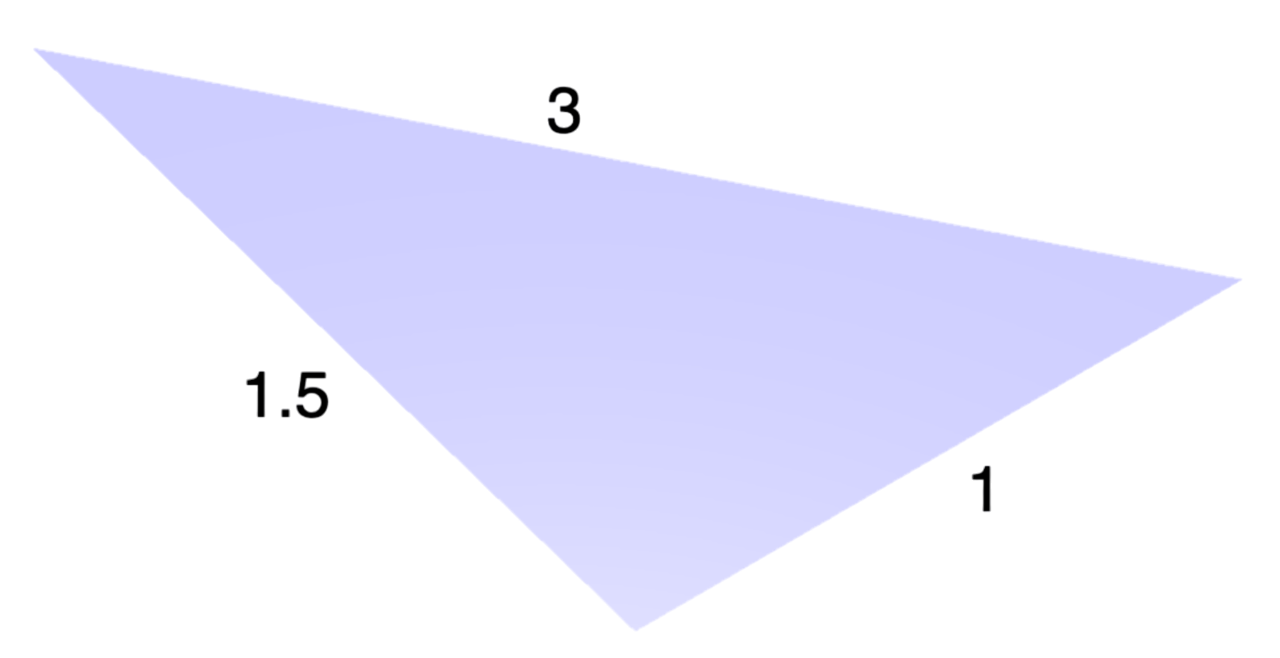
\includegraphics[width=0.9\columnwidth]{../images/cone_coordinate.png}
        \captionof{figure}{A non-planar triangle with edge lengths shown. Do not get fooled by the fact that it is being drawn in a plane - lengths are not to scale. The plane is merely the coordinate representation of the surface.}
        \label{fig:non-planar-triangle}
    \end{center}
    \begin{center}    
        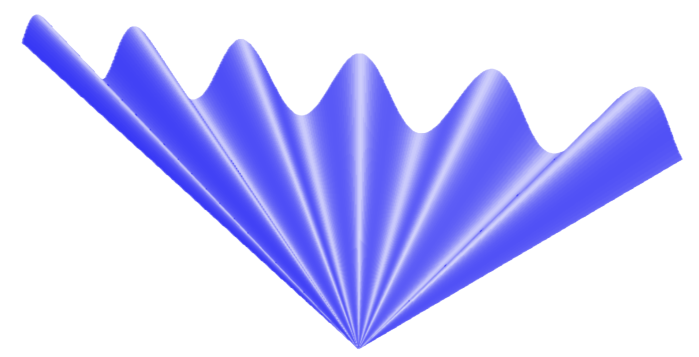
\includegraphics[width=0.8\columnwidth]{../images/fan.png}
        \captionof{figure}{A Euclidean embedding of the non-planar triangle requires curved geometry, as the triangle inequality is not satisfied. This figure shows one interpretation of a manifold that would result in the non-planar measurements.}\label{fig:fan_euclid}
    \end{center}
}
\example{Extrinsic vs Intrinsic Triangulation of the Fan model}{
    \begin{center}    
        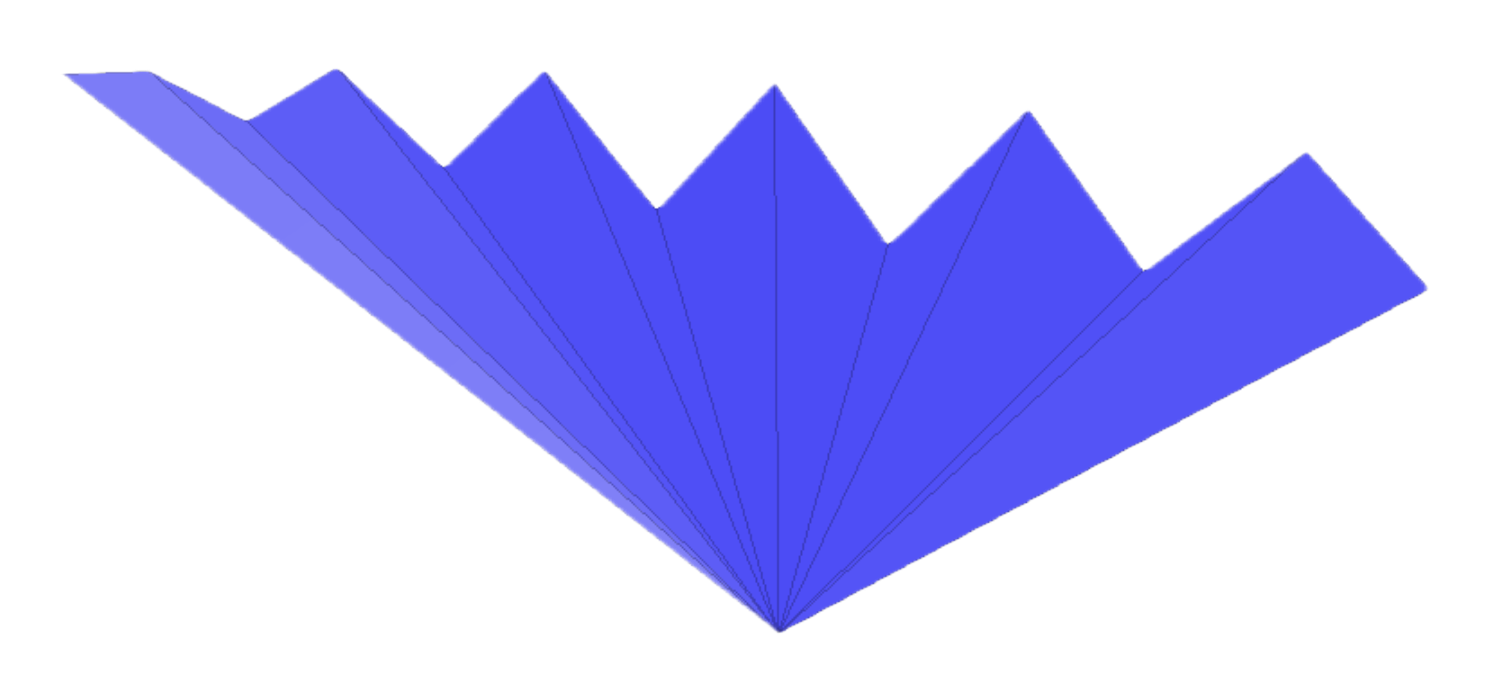
\includegraphics[width=0.8\columnwidth]{../images/fan_extrinsic.png}
        \captionof{figure}{An extrinsic 12-triangle isometrically embedded approximation of the fan model. The mesh stores only vertex positions. In ambient space, each vertex "sits" exactly on the manifold, while the planes spanned inbetween are linear approximations and will generally move away from the manifold.}
    \end{center}
    \begin{center}    
        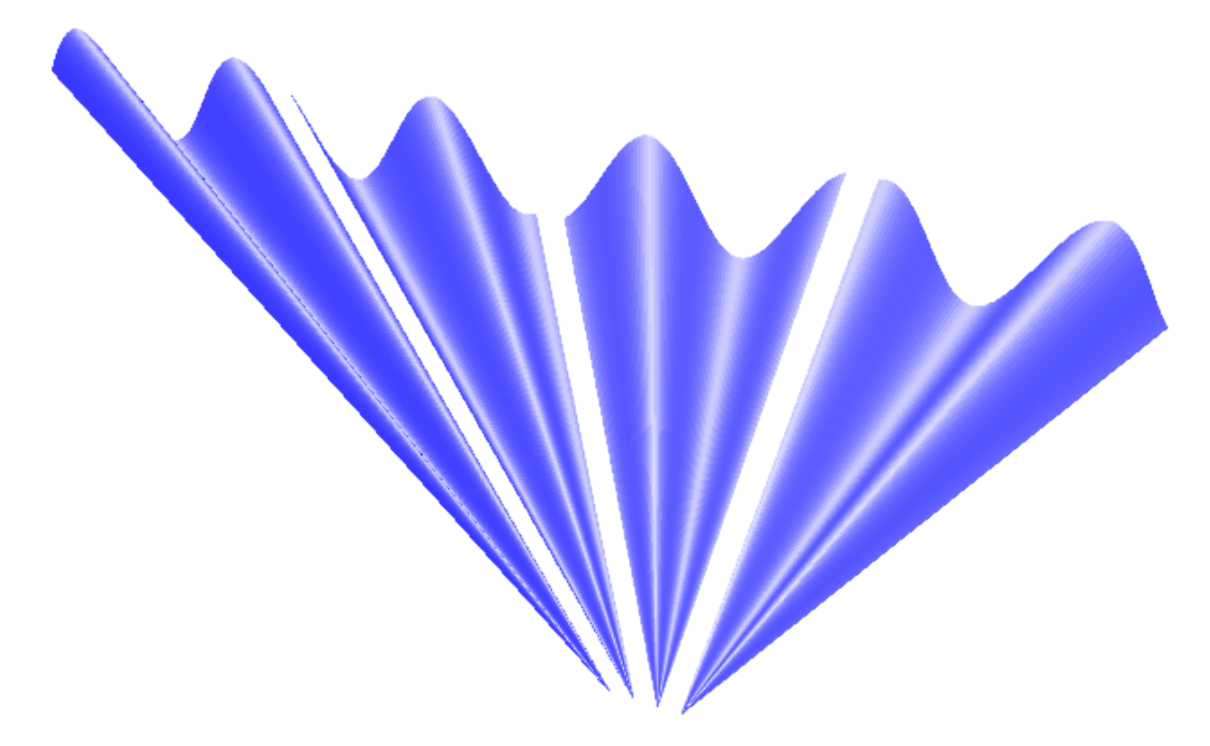
\includegraphics[width=0.8\columnwidth]{../images/fan_intrinsic.png}
        \captionof{figure}{An intrinsic 4-triangle representation of the fan model. The mesh stores edge-lengths only. We render the triangulation onto the Euclidean embedding (fig \ref{fig:fan_euclid}) to highlight the fact that edge-lengths are measured along the manifold, not in straight lines through ambient space. The manifold has been cut along the 3 edges of the 4-triangle mesh to show how it is implicitly partitioned.}
    \end{center}
}\noindent
We will now give our algorithm that builds the intrinsic triangulation. The algorithm is split into two phases: setup and refinement. The setup phase will compute the edge-lengths of the initial mesh and mark triangles that are non-planar, have edges that are too long or too short, or have an area that is too large. The refinement phase will then iteratively split the longest edge of the marked triangles and inspect the new triangles for the same properties. The algorithm will terminate after a fixed number of iterations or when there are no more marked triangles.
\algorithmbox{Setup Intrinsic Triangulation}{
    \textbf{Input:} $\vspace{3mm}$
    \\$M$ : Initial mesh that partitions the coordinate space $C$. $\vspace{1mm}$
    \\$g$ : Metric, mapping from any point in $C$ to 2x2 matrix.$\vspace{1mm}$
    \\$\rho$ : Desired maximal edge ratio in any triangle, $1 < \rho < 2$ $\vspace{1mm}$
    \\$A_{\text{max}}$ : Desired maximal area of any triangle.
    \\$\vspace{3mm}$%
     \textcolor[RGB]{170,170,170}{\rule{\linewidth}{0.4pt}}
    \transparent{0.5}%
    \textit{Step 1: Compute edge-lengths.} $\vspace{2mm}$
    \transparent{1.0}
    \\\textbf{for each} edge $E_i = (A, B)$ \textbf{in} $M$: $\vspace{2mm}$
    \begin{adjustwidth}{10px}{}
        Numerically compute the edge-length as \\$e_i = m(A, B)$\\
    \end{adjustwidth}
    \transparent{0.5}%
    \textit{Step 2: Inspect triangles.} $\vspace{2mm}$
    \transparent{1.0}
    \\Initialize \textbf{T} as the empty set $\vspace{2mm}$
    \\\textbf{for each} triangle $T$ \textbf{in} $M$: $\vspace{2mm}$
    \begin{adjustwidth}{10px}{}
        Add $T$ to \textbf{T} if
        \begin{adjustwidth}{10px}{}
            $T$ is not planar or
            \\
            the ratio $e_{\text{long}}/e_{\text{short}}$ exceeds $\rho$ or
            \\
            the area exceeds $A_{\text{max}}$
            \\$\vspace{-2mm}$%
        \end{adjustwidth}
    \end{adjustwidth}
    $\vspace{2mm}$%
     \textcolor[RGB]{170,170,170}{\rule{\linewidth}{0.4pt}}
    \\\textbf{Output:} $\vspace{2mm}$
    \\$\mathbf{\Delta}_0$ : Mesh $M$ with computed edge-lengths. $\vspace{1mm}$
    \\\textbf{T} : Set of marked triangles.
}\noindent
For the subsequent refinement phase, it will be useful to have a figure to refer to that explains the naming.
\definition{Local Triangle Naming scheme}{For a given triangle, we refer to edges as $E_{\text{long}}, E_{\text{medium}}, E_{\text{short}}$ with the property $e_{\text{long}} \geq e_{\text{medium}} \geq e_{\text{short}}$. \\The vertex opposing $E_{\text{long}}$ edge is \underline{\textbf{C}}orner, the vertex on the shortest edge \underline{\textbf{S}}hort, and the remaining vertex on the medium-length edge \underline{\textbf{M}}edium. The vertex across $E_{\text{long}}$ in a potential adjacent triangle is \underline{\textbf{O}}pposite. \\In the figure below, let $T$=SMC be the reference triangle. We have $E_{\text{long}}$=SM, $E_{\text{medium}}$=CM, and $E_{\text{short}}$=CS.
\vspace{-5mm}\begin{center}    
    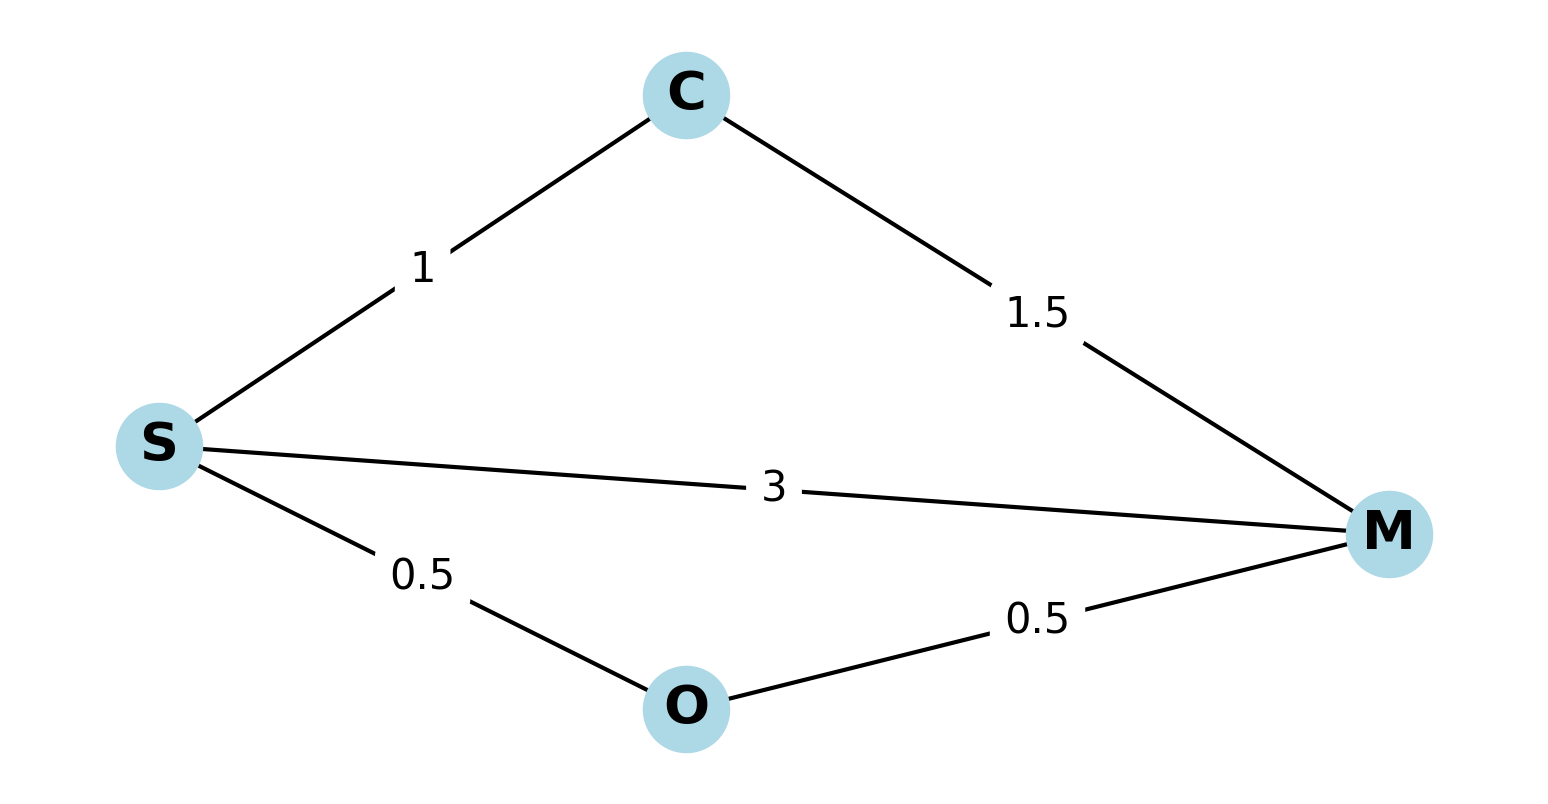
\includegraphics[width=1\columnwidth]{../images/mesh_refine_1.png}
    \captionof{figure}{The reference triangle patch illustrating  the naming scheme of the upcoming algorithms. This figure additionally serves as an example output $\mathbf{\Delta}_0$ of the setup phase. Both triangles would be in the output \textbf{T} due to their non-planarity.}
    \label{fig:naming_scheme}
\end{center}
}
\algorithmbox{Refine Intrinsic Triangulation}{
    \textbf{Input:} $\vspace{3mm}$
    \\$\mathbf{\Delta}_0$ : Initial intrinsic triangulation with edge-lengths. $\vspace{1mm}$
    \\\textbf{T} : Set of marked triangles.$\vspace{1mm}$
    \\$g$, $\rho$, $A_{\text{max}}$: As described in setup.$\vspace{1mm}$
    \\$\textbf{i}_{max}$ : Maximal number of subdivisions.
    \\$\vspace{3mm}$%
    \textcolor[RGB]{170,170,170}{\rule{\linewidth}{0.4pt}}
    \textbf{i} $\leftarrow$ 0$\vspace{2mm}$
    \\\textbf{while} \textbf{T} is not empty \textbf{and} \textbf{i} $<$ $\textbf{i}_{max}$:  $\vspace{2mm}$
    \begin{adjustwidth}{10px}{}            
            \textbf{i} $\leftarrow$ \textbf{i} + 1$\vspace{2mm}$
            \\
            Select the marked triangle $T=SMC\in\textbf{T}$ with the largest perimeter and remove $T$ from \textbf{T}.
            \\\\
            \transparent{0.5}%
            \textit{Step 1: Split longest edge.}$\vspace{2mm}$
            \transparent{1}
            \\
            Find Euclidean midpoint of longest edge $E_{\text{long}}$, define it as new vertex at $N$. $\vspace{2mm}$
            \\
            Remove previous edge $MS$, insert new edges $NS$, $MN$. $\vspace{2mm}$
            \\
            With metric $g$, compute $|NS| = m(N, S)$ and $|MN| = e_{\text{long}} - |NS|$$\vspace{2mm}$
            \\\\
            \transparent{0.5}%
            \textit{Step 2: Bisect faces.} $\vspace{2mm}$
            \transparent{1.0}
            \\
            Split $T$ and the adjacent triangular face $T^\prime$=SOM opposite $E_{\text{long}}$ to get triangles $SON$, $NOM$, $NMC$, $NCS$.$\vspace{2mm}$
            \\
            Remove $T^\prime$ from \textbf{T}. $\vspace{2mm}$ 
            \\
            Compute new edge-lengths $CN$ and $NO$: $|CN| = m(C, N)$, $|NO| = m(N, O)$. $\vspace{1mm}$$\vspace{2mm}$
            \\\\
            \transparent{0.5}%
            \textit{Step 3: Inspect new triangles.} $\vspace{2mm}$
            \transparent{1.0}
            \\
            Evaluate the planarity, area, and aspect ratio of $SON$, $NOM$, $NMC$, and $NCS$. $\vspace{2mm}$
            \\
            Based on planarity, $\rho$, and $A_{\text{max}}$, mark triangles for refinement by adding them to \textbf{T}.
            \\$\vspace{-2mm}$%
    \end{adjustwidth}
    \textcolor[RGB]{170,170,170}{\rule{\linewidth}{0.4pt}}$\vspace{2mm}$\\
    \textbf{Output:} $\vspace{2mm}$
    \\
    $\mathbf{\Delta}$ : Refined Intrinsic Triangulation, everywhere satisyfing the triangle inequality$\vspace{1mm}$
}\noindent
During subdivision, we are constructing an intrinsic partition of the manifold into triangles. A triangle might require multiply bisections before it becomes planar. Note that, before any splitting, we didn't have just a bad approximation - we had \textit{no} approximation. Splitting was necessary to work with the geometry.  
\newpage
\subsection*{Results}
\subsubsection*{Triangulating Gaussian Bump}
We define our own metric similarly to the hemisphere metric example in section \ref{sec:manifolds}.
The map $f$ from coordinate space $C = (-1, 1) \times (-1, 1)$ is given as 
$$f(\begin{pmatrix}
    x \\ y
\end{pmatrix}) = $$
$$\exp\left(-\left(\begin{pmatrix}
    x & y
\end{pmatrix} \begin{bmatrix} 0.1 & 0.1 \\ 0.1 & 0.35 \end{bmatrix} \begin{pmatrix}
    x \\ y
\end{pmatrix}\right)^2\right)$$
Figure \ref{fig:bell_input} shows the initial coarse mesh. The algorithm is run for $500$ steps with $A_{\text{max}} = 1/8$ and $\rho = 1.2$. The output is shown in figures \ref{fig:bell_tissot}. The mesh is now more dense around the peak of the bump, where the curvature is higher. The mesh is not an embedding of the manifold, but an intrinsic triangulation. An embedding using $f$ is shown in fig \ref{fig:bell_embedded}, giving an extrinsic representation. We might not generally have access to $f$, and this figure is for illustration purposes only. Notice that triangles that appear very thin and stretched in the intrinsic triangulation are not so after being embedded isometrically.
\begin{figure}
    \centering
    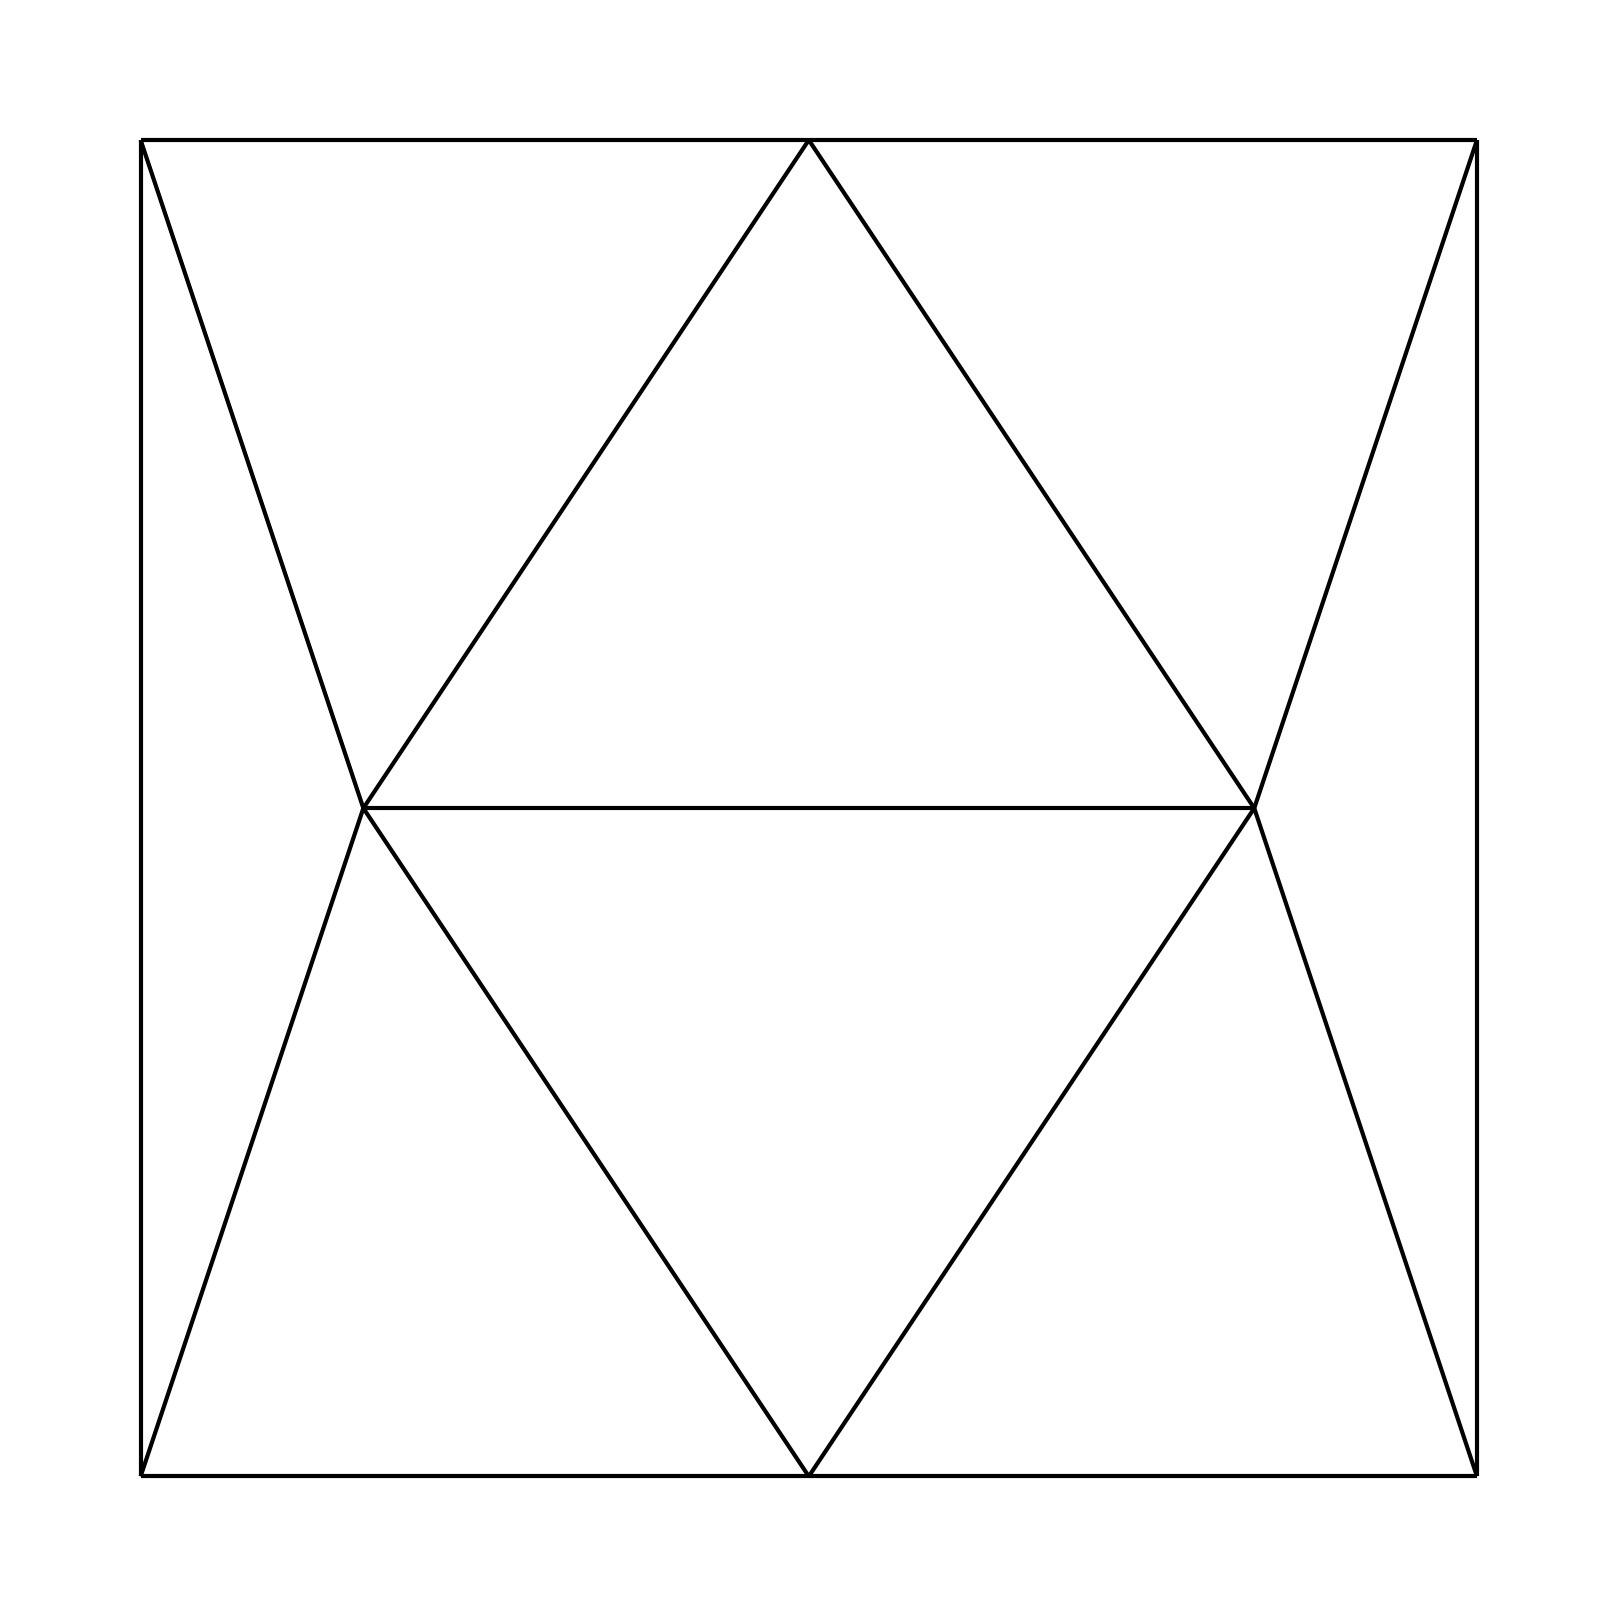
\includegraphics[width=0.75\columnwidth]{../images/bell_before_refinement.png}
    \captionof{figure}{Input mesh.}
    \label{fig:bell_input}
    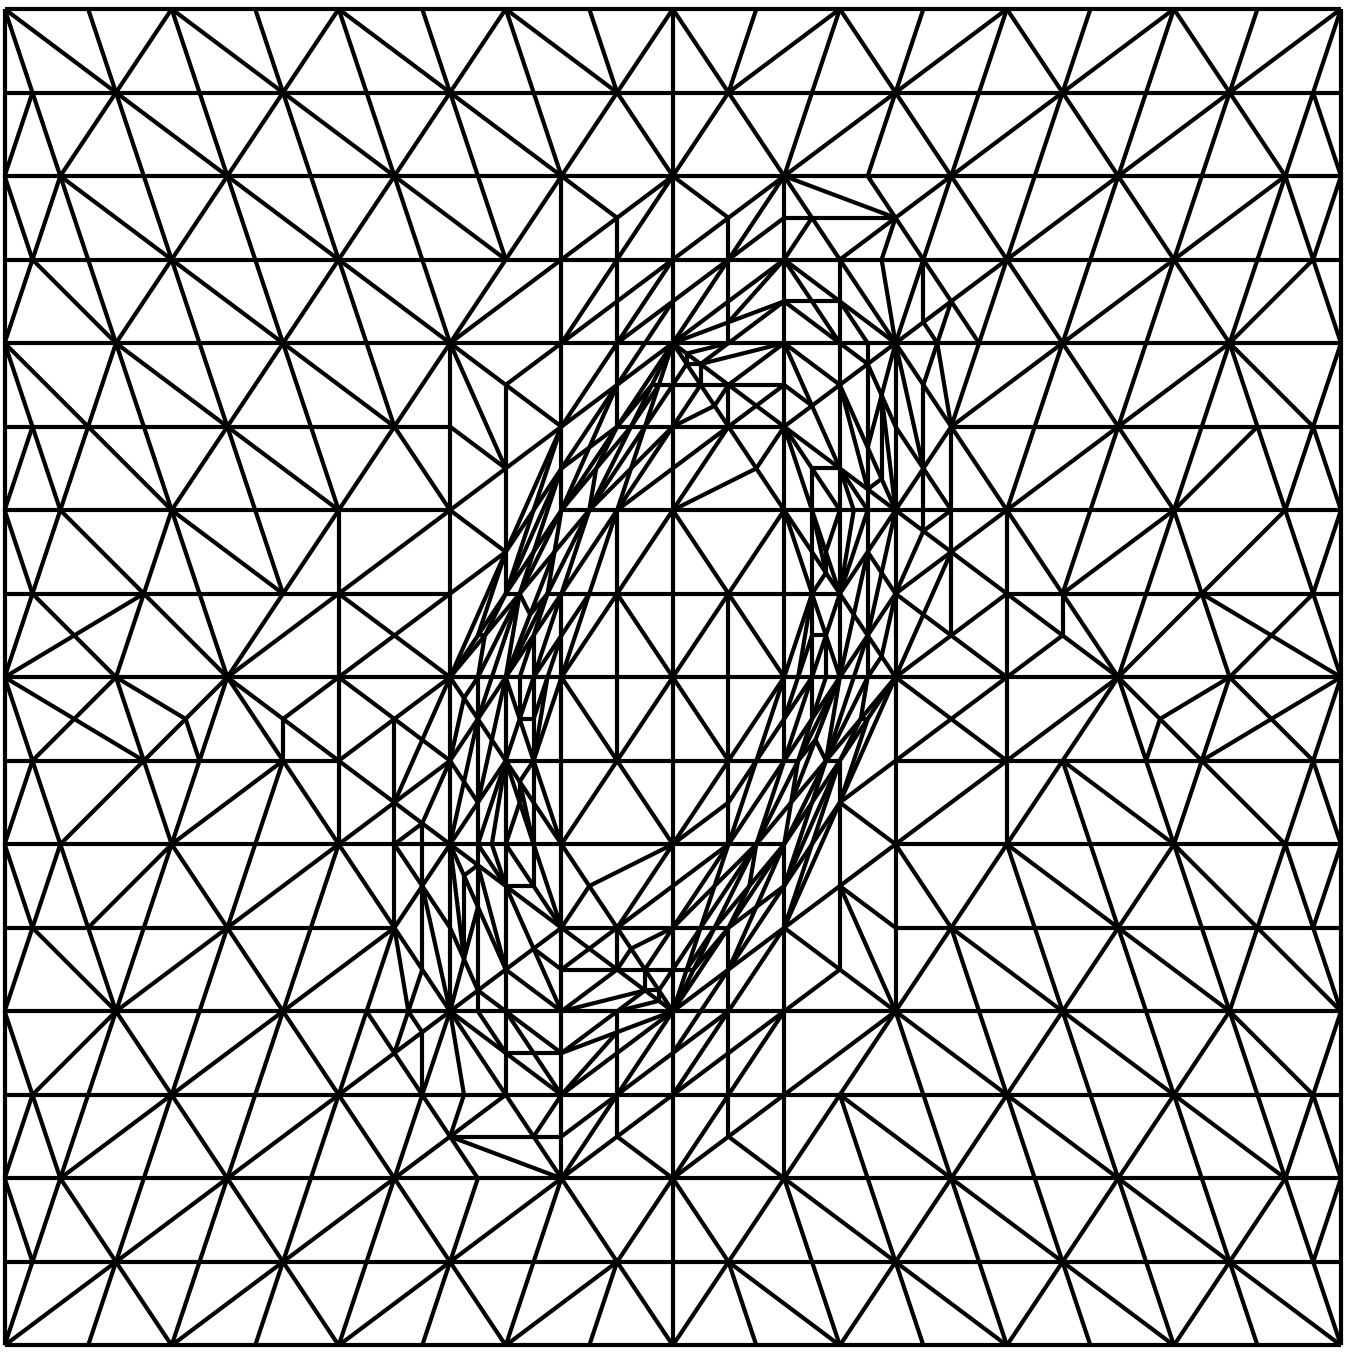
\includegraphics[width=0.75\columnwidth]{../images/bell_after_refinement.png}
    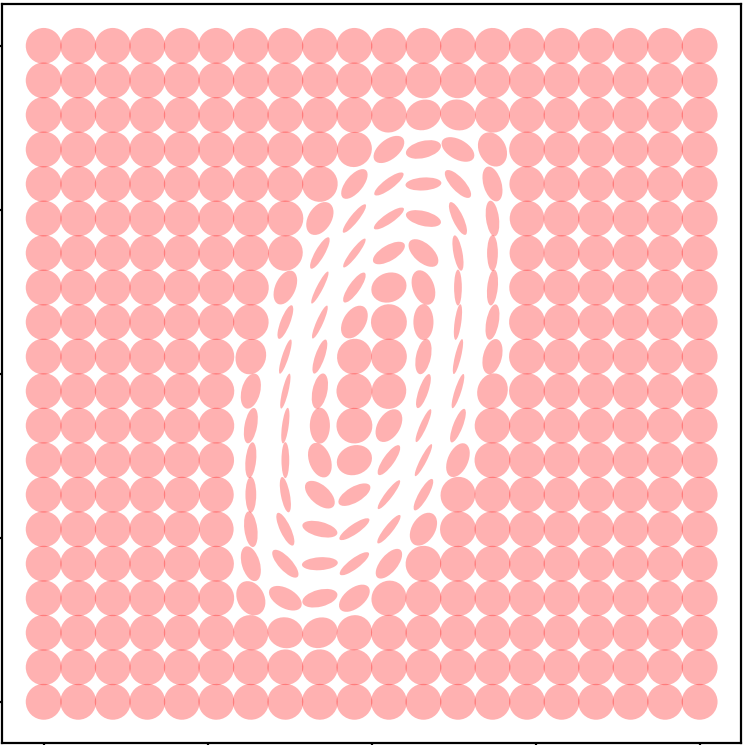
\includegraphics[width=0.75\columnwidth]{../images/bell_tissot.png}
    \captionof{figure}{Output mesh and Tissot's indicatrices.}
    \label{fig:bell_tissot}
    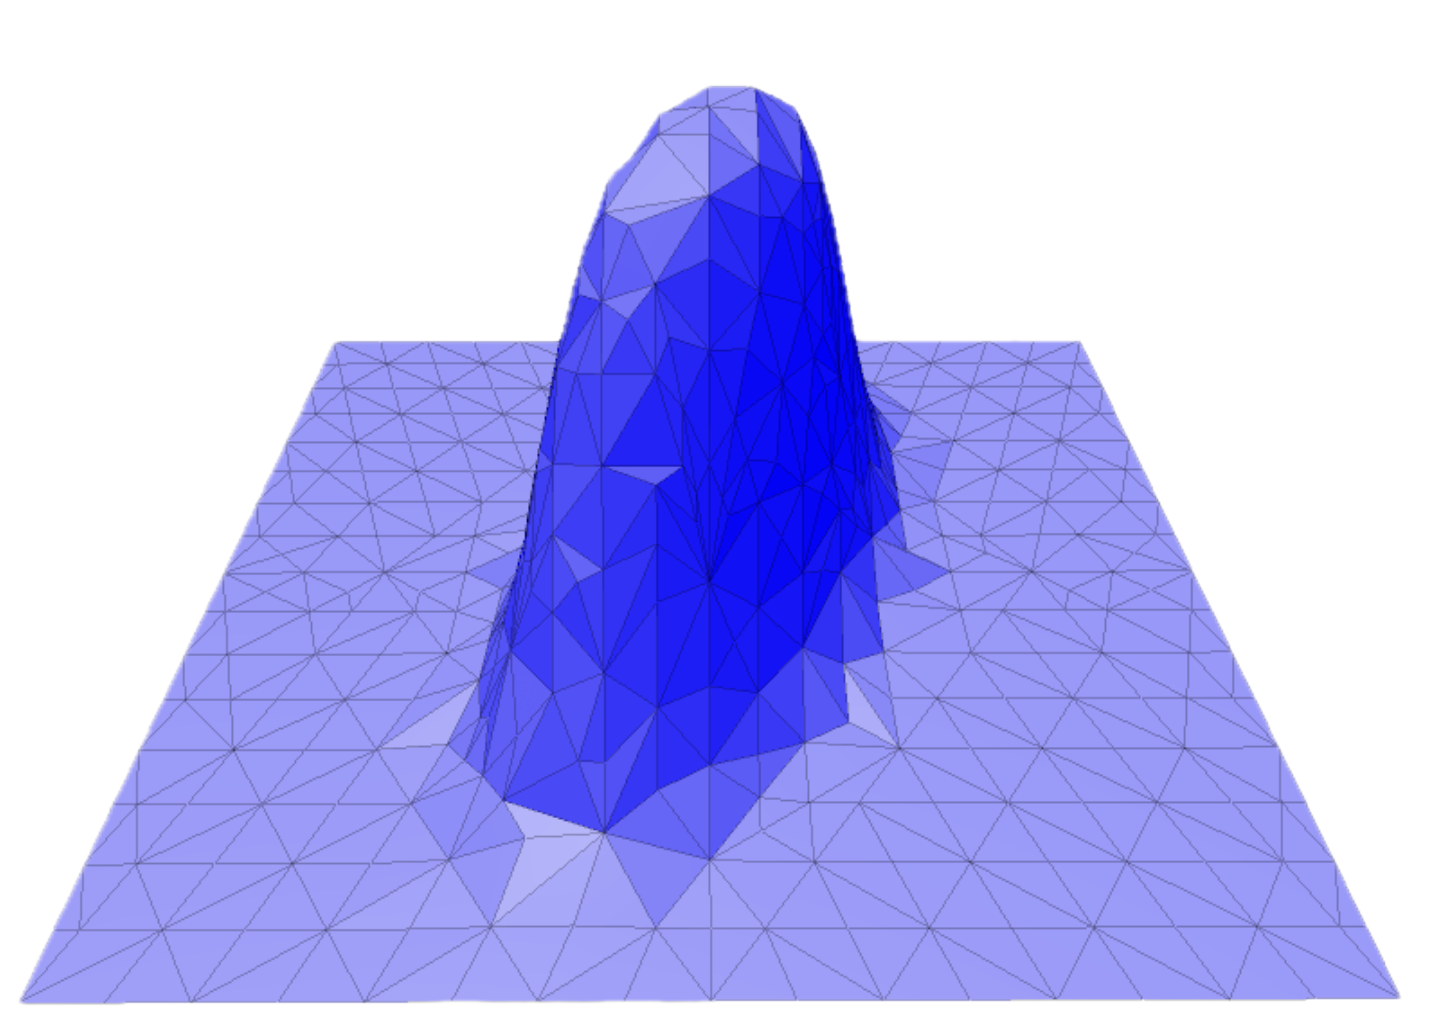
\includegraphics[width=0.94\columnwidth]{../images/bell_embedded.png}
    \captionof{figure}{Mapping the refined mesh through the embedding function $f$.}
    \label{fig:bell_embedded}
\end{figure}

\subsubsection*{Triangulating subset of the Hyperbolic Plane}
    We showcase the algorithm on the Poincaré disc model of $\mathbb{H}^2$ and compare with a hyperbolic tiling. As discussed in an earlier section, we cannot triangulate an unbounded domain, so we truncate the unit disc and look only within the disc of radius $0.97$. Algorithm run for $500$ steps with $A_{\text{max}} = \infty$ and $\rho = 1.9$. Setting $A_{\text{max}} = \infty$ leads to the parameter being ignored, while a high setting of $\rho$ makes the refinement phase focus just on making planar triangles, which means that all initial iterations are likely to focus on non-planar triangles only. 
    \\
    Figure \ref{fig:hyper_before} shows the input mesh $\mathbf{\Delta}_0$, which covers the $0.97$-disc somewhat uniformly. Three triangles on the way to the border have their edge-lengths marked. This is the length under the hyperbolic metric. The outermost triangle does not satisfy the triangle inequality in this initial mesh, as $1.34 + 2.04 < 6.08$. Figure \ref{fig:hyper_after} shows the output of the algorithm, an intrinsic triangulation of a subset of $\mathbb{H}^2$. The high triangle density at the edges highlights the hyperbolic expansion of space, which necessitates triangle subdivision. All triangles are congruent. The triangles in our tiling are not congruent and will depend on the initial triangulation, but $A_{\text{max}}$ ensures that we make splits around the edge proportional to the area. A common visualization of the hyperbolic plane is given in fig \ref{fig:hyper_tiling}, in which all triangles are congruent. This visualization bears resemblance to the one obtained in figure \ref{fig:hyper_after} and illustrates the hyperbolic expansion of space which necessitates triangle subdivision.
    \\
    \begin{figure}
        \centering
        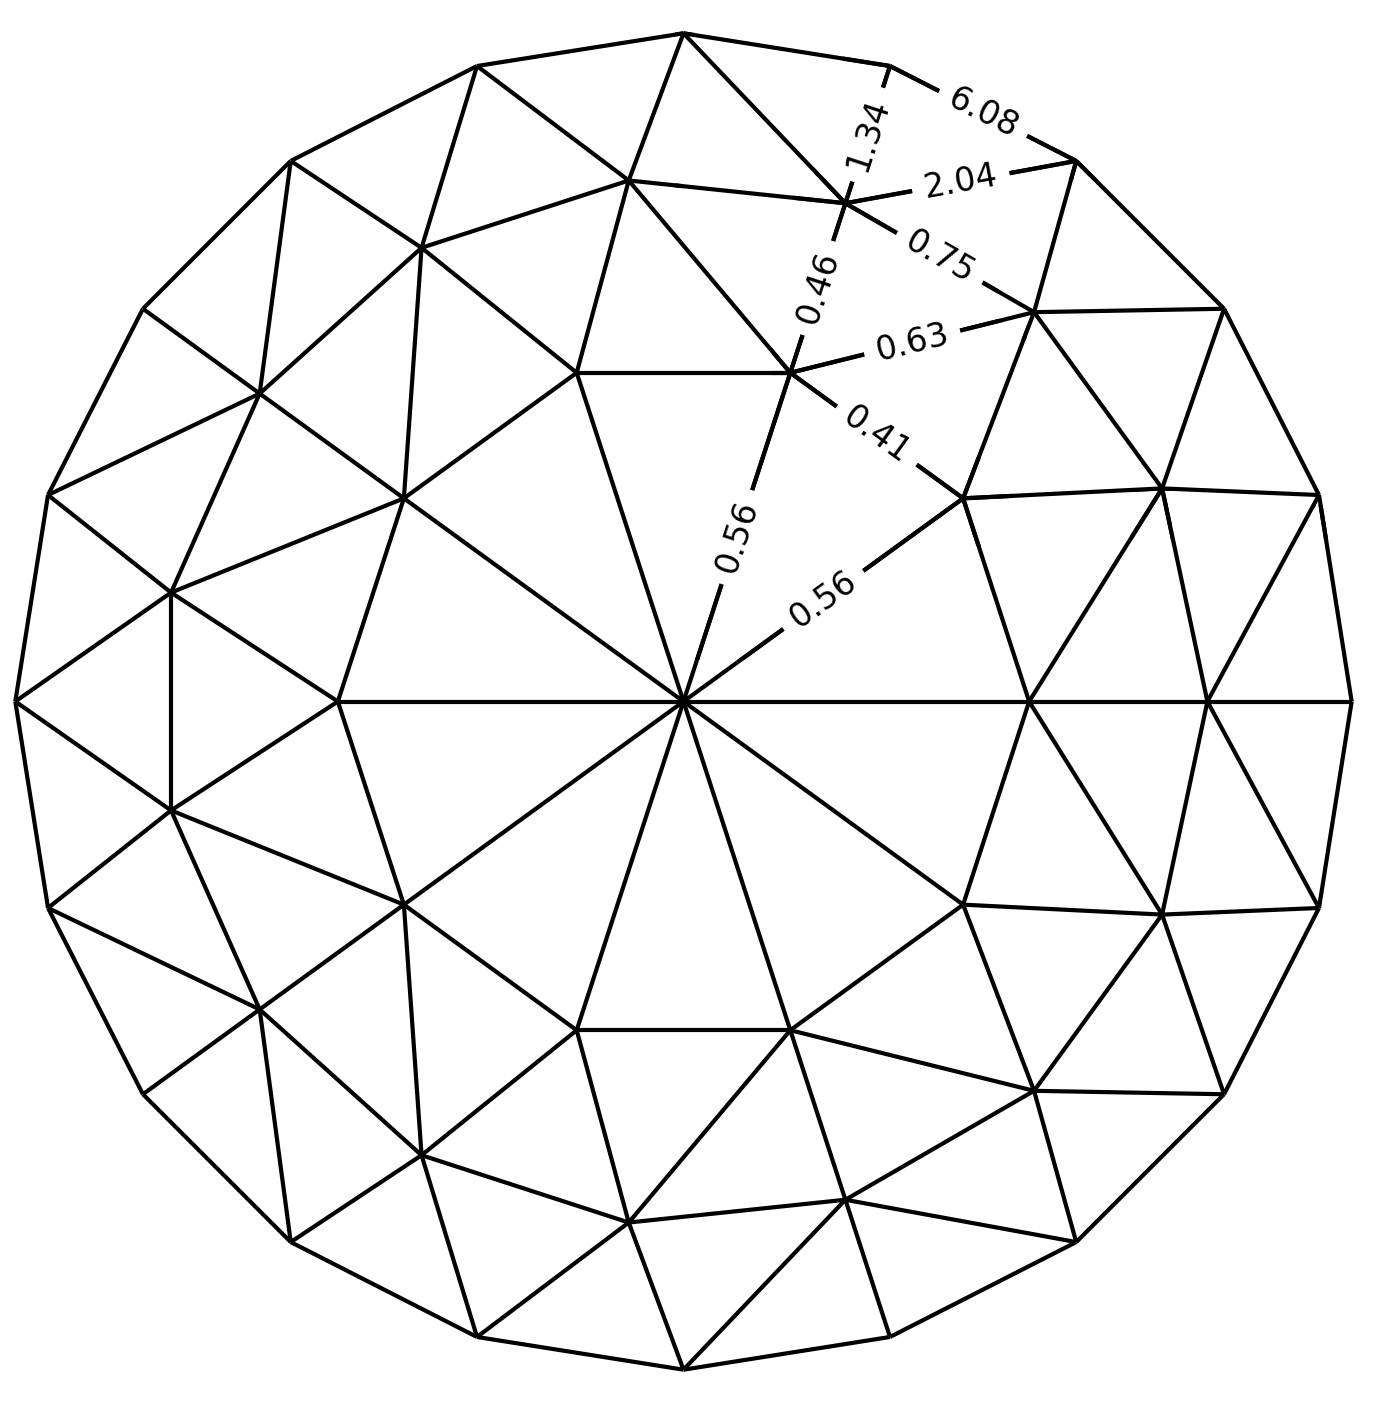
\includegraphics[width=0.85\columnwidth]{../images/hyperbolic_disc_before_refinement_some_labels.png}
        \captionof{figure}{Input mesh.}
        \label{fig:hyper_before}
        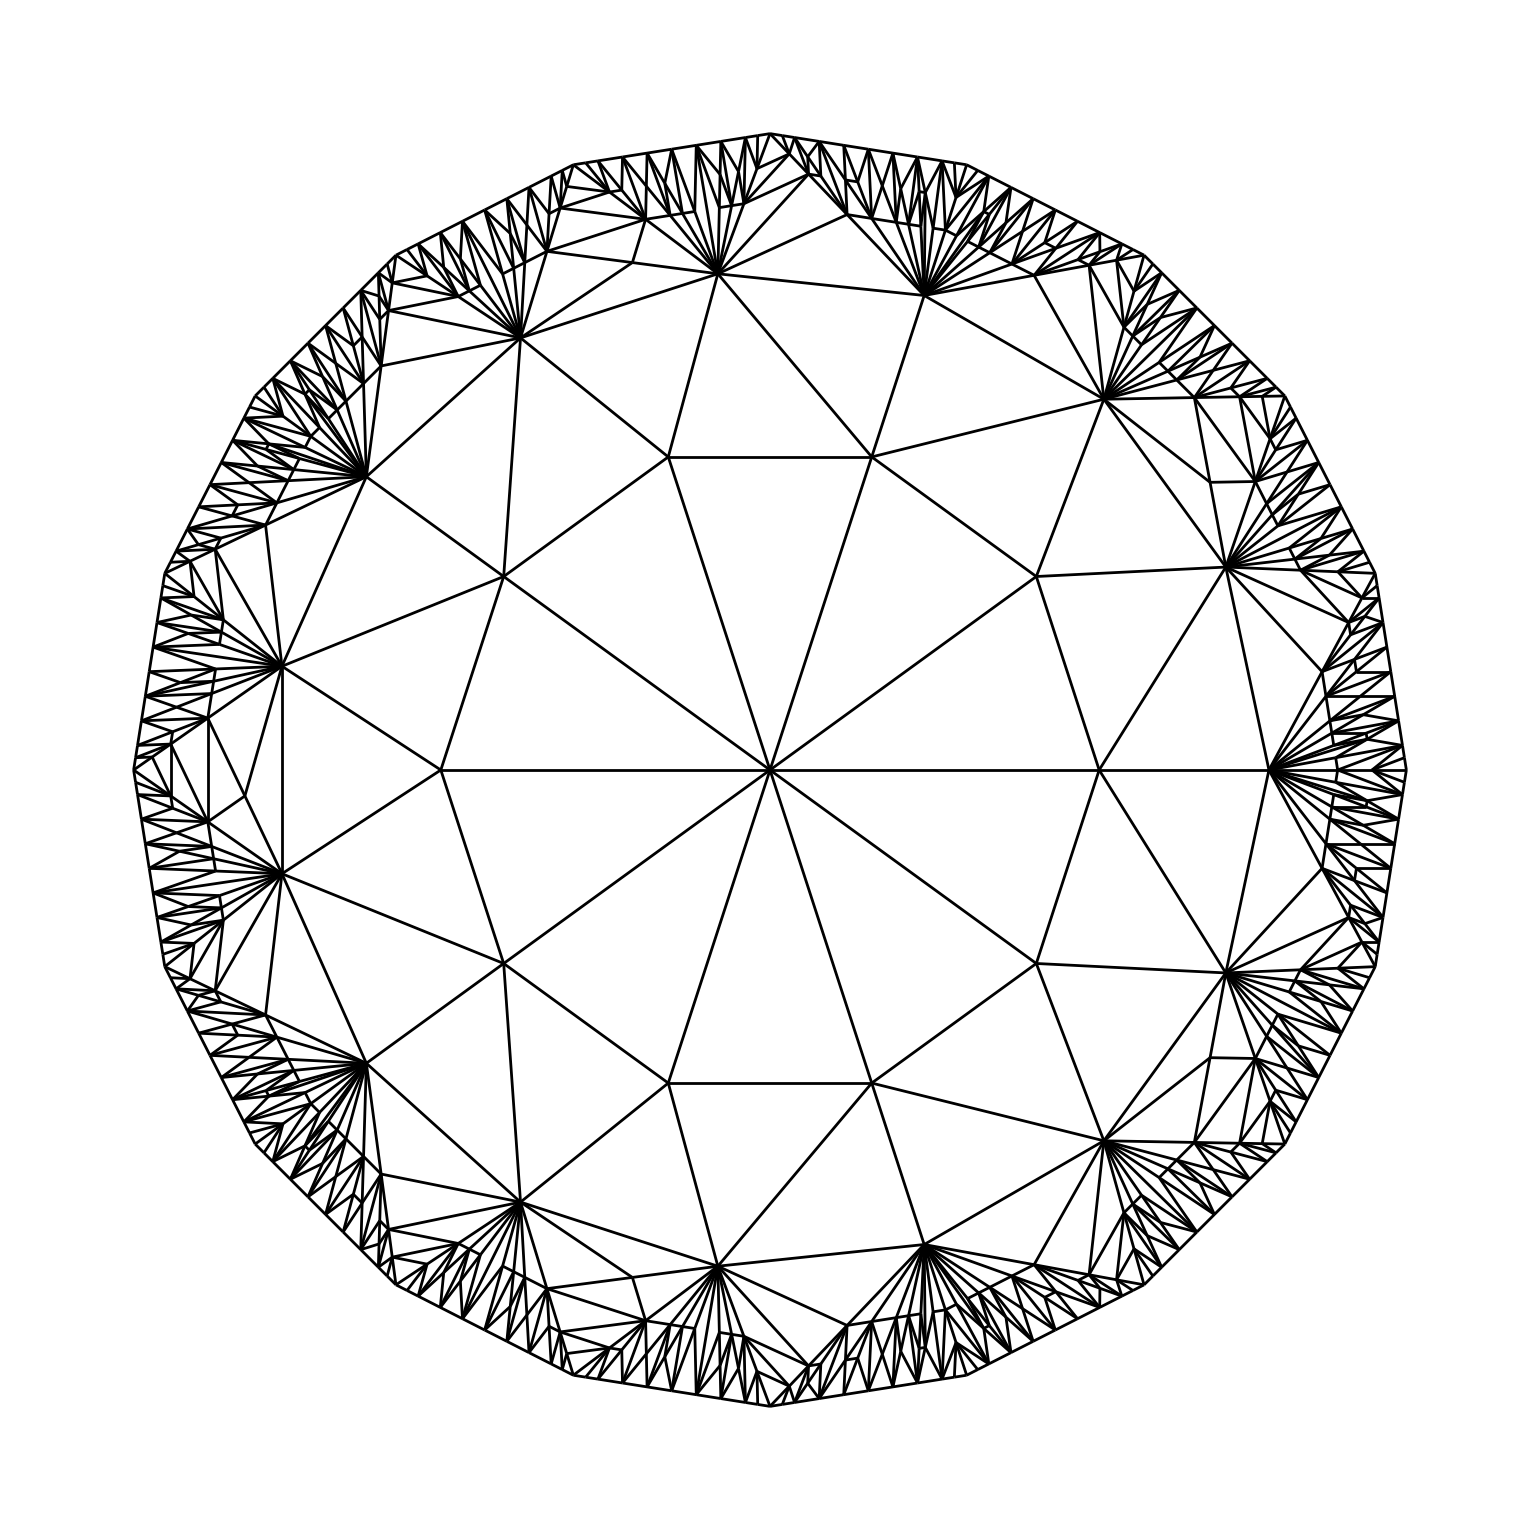
\includegraphics[width=0.85\columnwidth]{../images/hyperbolic_disc_after_refinement.png}
        \captionof{figure}{Output mesh}
        \label{fig:hyper_after}
        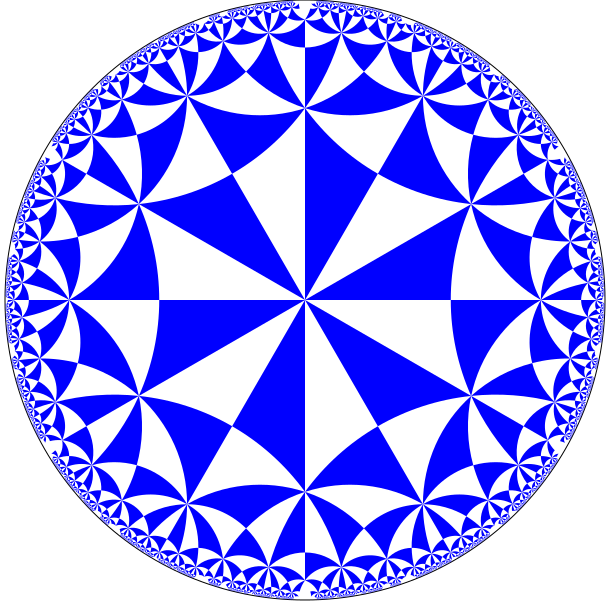
\includegraphics[width=0.85\columnwidth]{../images/wiki_hyperbolic.png}
        \captionof{figure}{Tiling of the hyperbolic plane from \cite{HyperbolicTiling}.}
        \label{fig:hyper_tiling}
        
    \end{figure}

\subsection*{Improvements}
One could, assuming the fan-model, also compute the distance from the midpoint of the longest edge to the opposing corner as $(1 + 1.5) / 2 = 1.25$. Under that assumption it will yield exact distances. This could be done as the last split in each triangle so the approximation error does not propagate.
\\\\ Additionally, instead of bisecting the longest edge at its Euclidean midpoint (in coordinate space), one can run an incremental search along it to determine the midpoint in coordinate space under the metric $g$. This which would be a more reasonable choice for the new vertex and might save a few subdivisions. It can even be done at the same cost of the current algorithm, since, once the midpoint is found, one will know that the lengths of the two constituent edges are equal and sum to the original length.
\\\\ The metric tensor will be evaluated in the same vertex many times if the edge is split multiple times. One could cache the metric tensor at each vertex to avoid redundant computations.
\\\\ After the refinement phase, one can run edge-flipping (\cite{sharp2021intrinsic}, \cite{intrinsic_laplacian}) to further improve the quality. This is an operation applicable to intrinsic triangulations that swaps diagonal edges of a quadrilateral if it improves the quality of the triangulation.
\\\\ Alternatively to edge-flipping, one could use a different subdivision scheme, such as red-green refinement. This is more complex, but might yield better results as it is free to place new vertices in the interior of the triangle, not just on the edges.
\\\\ Generally, the greedy subdivision scheme could be improved upon or replaced. If one zooms in on the picture in figure \ref{fig:bell_embedded}, one notices a so-called "rat-nest", which is a vertex with many incident edges. This is a common problem in greedy subdivision schemes, and will generally lead to elongated triangles. The bisection method can never get rid of a rat-nest after it has made one.

\ifdefined\COMPILINGFROMMAIN
\else
    \end{document}
\fi

\clearpage
\section{Partial Differential Equations and the Method of Lines}\label{sec:pde}
\ifdefined\COMPILINGFROMMAIN
\else
    %%%%HEADER
\documentclass[twocolumn]{article}
\usepackage[a4paper, margin=1in, columnsep=20pt]{geometry}
\usepackage{amsmath, amssymb, graphicx, hyperref}
\usepackage[most,skins,breakable]{tcolorbox}
\usepackage[symbol]{footmisc}
\usetikzlibrary{calc}
\usepackage{xcolor}
\usepackage{caption}
\usepackage{algorithm}
\usepackage{algpseudocodex}
\usepackage{tikz}
\usepackage{listings}
\usetikzlibrary{arrows.meta, positioning}
\tcbuselibrary{listingsutf8}
\usepackage{microtype}
\usepackage{blindtext}
\usepackage{bookmark}
\usepackage{breqn}
\usepackage[backend=biber,style=numeric]{biblatex} % 
\addbibresource{../references.bib}

% Define style for the listings environment
\lstdefinestyle{mystyle}{
    basicstyle=\ttfamily\small,
    breaklines=true,
    escapeinside={(*@}{@*)}, % Allows math mode within listings
    numbers=left,
    numberstyle=\tiny,
    frame=single,
    keywordstyle=\color{blue}\bfseries,
    commentstyle=\color{green!50!black},
    stringstyle=\color{red}
}


\def\reals{\mathbb{R}}
% Define the custom definition box and command
\newtcolorbox{mydefinition}[2][]{%
    text width=0.95\columnwidth,
    before=\vspace{1mm}, 
    after=\vspace{1mm}, 
    colback=gray!10, % Background color (light gray)
    colframe=black!70,  % Border color
    coltitle=gray!10,  % Title color
    fonttitle=\bfseries, % Title font style
    sharp corners,   % Box style
    left=2pt,
    breakable,
    right=2pt,
    top=2pt,
    bottom=2pt,
    enhanced jigsaw,
    title=Definition: {#1},         % Title passed as the first argument
    colupper=black,  % Ensure proper content handling
    pad at break*=1pc,
    overlay first and middle={
        \coordinate (A1) at ($(interior.south east) + (-10pt,5pt)$);
        \coordinate (C1) at ($(interior.south east) + (-6pt,7.5pt)$);
        \draw[fill=black!50] (A1) -- +(0,5pt) -- (C1) -- cycle;
    }
    }
    
\newcommand{\definition}[2]{%
    \noindent%
    \begin{mydefinition}[#1]%
        .#2%
    \end{mydefinition}%
    \noindent
}

\newtcolorbox{myexample}[2][]{%
    text width=0.95\columnwidth,
    before=\vspace{1mm}, 
    after=\vspace{1mm}, 
    colback=orange!3, % Background color (light gray)
    colframe=black!70,  % Border color
    coltitle=gray!10,  % Title color
    fonttitle=\bfseries, % Title font style
    sharp corners,   % Box style
    left=2pt,
    right=2pt,
    top=2pt,
    bottom=2pt,
    breakable,
    title=Intuition: {#1},         % Title passed as the first argument
    pad at break*=1pc,
    overlay first and middle={
        \coordinate (A1) at ($(interior.south east) + (-10pt,5pt)$);
        \coordinate (C1) at ($(interior.south east) + (-6pt,7.5pt)$);
        \draw[fill=black!50] (A1) -- +(0,5pt) -- (C1) -- cycle;
    }
}

\newcommand{\example}[2]{%
    \noindent%
    \begin{myexample}[#1]%
    .#2%
    \end{myexample}%
    \noindent
}

\newtcolorbox{algobox}[2][]{%
    text width=0.95\columnwidth,
    before=\vspace{1mm}, 
    after=\vspace{1mm}, 
    colback=blue!5, % Background color (light gray)
    colframe=black!70,  % Border color
    coltitle=gray!10,  % Title color
    fonttitle=\bfseries, % Title font style
    sharp corners,   % Box style
    left=2pt,
    right=2pt,
    top=2pt,
    bottom=2pt,
    breakable,
    title=Algorithm: {#1},         % Title passed as the first argument
    pad at break*=1pc,
    overlay first and middle={
        \coordinate (A1) at ($(interior.south east) + (-10pt,5pt)$);
        \coordinate (C1) at ($(interior.south east) + (-6pt,7.5pt)$);
        \draw[fill=black!50] (A1) -- +(0,5pt) -- (C1) -- cycle;
    }
}

\newcommand{\algorithmbox}[2]{%
\noindent%
    \begin{algobox}[#1]%
    .#2%
    \end{algobox}%
    \noindent
}
%%%%HEADER

    \begin{document}
\fi

\definition{Ordinary Differential Equation, First Order}{
    An ordinary differential equation (ODE) is a differential equation where the solution $u: \reals \to \reals^n$ is defined implicitly by relating it to its own derivatives through $f: \reals^n \to \reals$:
        $$\frac{d}{dt}u(t) = f(u(t))$$
    $u$ is a function of only one scalar variable (usually interpreted as time $t$), and $f$ is a function depending on $u$. If the ODE is vector valued, one also refers to solving it as integrating a vector field $f$.
}
Authors will often omit the explicit dependence on $t$ and write $\frac{d}{dt}u = f(u)$\footnote{This is abbreviation is similar to how one might write the equation $h(a) = f(a) + 3\cdot g(a)$ as $h(a) = (f+3g)(a)$ or $h = f+g$, treating functions as members of a vector space.}. It is implied that this relation must hold for all times $t$.
\definition{Order of ODE}{
    The order of an ODE is the degree of the highest derivative of $u$ involved in the equation. An $n$'th ODE can be written as $$\frac{d^n}{dt^n}u(t) = f(u(t), u^{(1)}(t), \dots, u^{(n-1)}(t))$$
} TODO Time invariant autonomous
We can always rewrite an $n$'th order ODE into a system of $n$ first-order ODEs, which is useful as one then need not engineer a new solution method for each choice of $n$.
\example{Converting a $n$th order ODEs to system of first-order ODEs}{
Suppose we have the $n$th order ODE
\begin{align} \label{eq:high_order_ode}
    \frac{d^n}{dt^n}u = f(u, u^{(1)}, \dots, u^{(n-1)})
\end{align}
By defining $n-1$ auxiliary functions $v_i$ for $i\in\{1, \dots, n-1\}$
\begin{align*}
    \frac{d}{dt}u &= v_1
    \\
    \frac{d}{dt}v_i &= v_{i+1} 
\end{align*}
We may equivalently express \ref{eq:high_order_ode} as 
\begin{align*}
    \frac{d}{dt}u &= v_1
    \\
    \frac{d}{dt}v_1 &= v_2
    \\ 
    \vdots
    \\
    \frac{d}{dt}v_{n-2} &= v_{n-1}
    \\ 
    \frac{d}{dt}v_{n-1} &= f(u, v_1, \dots, v_{n-1})
\end{align*}
which can be interpreted as a vector valued first order ODE with solution $\vec{u}$
\begin{align}\label{eq:stack}
    \frac{d}{dt}\vec{u} = \frac{d}{dt}\begin{pmatrix}
        u \\ v_1 \\ \vdots \\ v_{n-1}
    \end{pmatrix} = \begin{pmatrix}
        v_1 \\ v_2 \\ \vdots \\ f(u, v_1, \dots, v_{n-1})
    \end{pmatrix}
\end{align}
}\noindent
If $f$ is a linear function of $u$ and its derivatives, the ODE is linear. The right-hand side of \ref{eq:stack} can then expressed as a matrix-vector product.
\example{2nd order \textit{Linear} ODE to first-order ODEs}{
We inspect the scalar second order linear ODE\footnote{This is the dampened harmonic oscillator (a one-dimensional spring model). $k$ represents the spring stiffness constant from Hooke's law, and $l$ is a damping coefficient that brings the system to a halt over time. With this physical perspective, one can mentally rename $u(t)$, $u'(t)$, and $u''(t)$ respectively to the more descriptive names $p(t)$ (position), $v(t)$ (velocity), and $a(t)$ (acceleration).} with constants $k>0$ and $l>0$
$$\frac{d^2}{dt^2}u = -ku - l\frac{d}{dt}u(t)$$
The corresponding form of \ref{eq:stack} will turn out as
\begin{align}\label{eq:linear_stack}
    \frac{d}{dt}\vec{u} = \frac{d}{dt}\begin{pmatrix}
        u \\ v
    \end{pmatrix} &= \begin{pmatrix}
        v \\ -ku - lv
    \end{pmatrix} % TODO REMOVE LABEL
    \\\iff \frac{d}{dt}\begin{pmatrix}u \\ v\end{pmatrix} &= \begin{bmatrix} 0 & 1 \\ -k & -l \end{bmatrix} \begin{pmatrix}u \\ v\end{pmatrix}
    \\\iff \frac{d}{dt}\vec{u} &=A\vec{u}
\end{align}
The matrix $A$ captures the system dynamics. The '$1$' in the off-diagonal encodes the integral-derivative relationship between $u$ and $v$.
}
The derivative-stack solution $\vec{u}(t)$ of vector-valued ODE at time $t$ is referred to as its "state" at $t$. If one is only interested in the solution $u(t)$ one can discard the remainder of the state.
\definition{Initial Value Problem for ODE}{
    Given the initial state $\vec{u}(0)$ and system dynamics $$\frac{d}{dt}\vec{u}(t) = A\vec{u}(t)$$ simulate the state evolution until final finite time $T$. Return either $\vec{u}(T)$ or the full trajectory $\vec{u}(t)$ for $t\in [0, T]$.
}
For Linear ODEs, closed form solutions to the initial value problem exist. They can be used as a reference to verify numeric solvers.
\example{Analytical solutions of First Order Linear ODEs}{
The linear scalar ODE with scalar coefficient $a$ $$\frac{d}{dt}u(t) = au(t) \hspace{20px}$$ has solution $$u(t) = \text{e}^{at}u(0)$$
This pattern generalizes to $n$-dimensional ODEs with matrix coefficient $A\in\reals^{n\times n}$
$$\frac{d}{dt}\vec{u}(t) = A\vec{u}(t)$$ 
which has the solution $$\text{e}^{At}\vec{u}(0)$$

$\text{e}^{At}$ is the matrix exponential, and is defined only for square matrices. $\text{e}^{At} = \sum_{n=0}^{\infty} \frac{t^n}{n!}A^n$. TODO VERIFY
}
Rarely can IVP problems be solved analytically, hence the need for numerical methods.
\definition{Numerical solution of ODE}{
    A numerical solution of an ODE is an approximation of $u(t)$ at finite timesteps $t \in \mathbb{T} = (0, t_1, t_2, \dots, T)$.
}
High regularity of $f$ will make it predictable, which gives better results. With a probabilistic solver, regularity of $u$ will be something we can control, independent of $f$. TODO cite convergence speeds.
\definition{Partial Differential Equation, $n$'th Order}{ TODO WHAT IS THE ORDER
    A partial differential equation (PDE) differs from an ODEs in that the solution $u$ can depend continuously on $d=|\{t,  x_1, \dots, x_{d-1}\}| = |\{t, \mathbf{x}\}|$   variables, $u: \reals^d \to \reals^n$. The total derivative $\frac{d}{dt}$ is replaced with the partial derivative $\frac{\partial}{\partial t}$ and  vector field $f: \reals^n \to \reals^d$ can additionally depend on the partial derivatives
    \begin{align*}
        \frac{\partial^n}{\partial t^n}u(t, \mathbf{x}) = f\Big(&u(t, \mathbf{x}),
        \\&\left\{\frac{\partial^q}{\partial t^q}u(t, \mathbf{x})\right\}_{q=1}^{n-1},
        \\&\left\{\frac{\partial^q}{\partial x^q}u(t, \mathbf{x}) \;:\; x\in \mathbf{x}\right\}_{q=1}^{\infty}\Big)
    \end{align*}
    In this thesis we generally work with PDEs over 2-dimensional space, so we have $\mathbf{x}\in \reals^2$ and time $t\in \reals$ as $u(t, \mathbf{x})$.
}
PDEs can make the time-evolution of a system depend on spatial properties such as the gradient and curvature. TODO: Define linear PDE. Define semilinear PDE
Often the domain $\mathcal{M}\ni \mathbf{x}$ has a border $\partial\mathcal{M}$ which the solution $u$ will have to interact with. The spatial partial derivatives in $f$ will be well-defined everywhere on the interior of $\mathcal{M}$ but not on $\partial\mathcal{M}$ and we will have to prescribe a value to make the problem well-posed.
We will cover two types of boundary conditions (BCs), the Dirichlet BC and Neumann BC. 
\definition{Dirichlet Boundary Conditions}{
    Dirichlet BCs prescribe the value of $u$ on the border with boundary values $g: \partial\mathcal{M} \to \reals$:
    \begin{align*}
        \frac{\partial}{\partial t}u(t, x) &= f(\cdot, \dots, \cdot ) & x\in \mathcal{M}
        \\
        u(t, x) &= g(x) & x\in \partial\mathcal{M}
    \end{align*} 
}
Dirichlet BCs amount to "pinning" the solution to a specific value at the boundary.
\definition{Neumann Boundary Conditions}{
    Neumann BCs prescribe the directional spatial derivative in the direction of the outer normal $n(x)$ of the boundary. Let $d: \partial\mathcal{M} \to \reals$:
    \begin{align*}
        \frac{\partial}{\partial t}u(t, x) &= f(\cdot, \dots, \cdot ) & x\in \mathcal{M}
        \\
        \nabla_x u(t, x)^\top n(x) &= d(x) & x\in \partial\mathcal{M}
    \end{align*}  TODO CHECK
}
Neumann BCs are a bit less intuitive, but allow one to set the "slope" at the boundary.
One simple instance of a PDE is the heat equation, which we will return to as a running example. It is defined with the Laplace operator, a differential operator involving partial derivatives. 
\example{Heat Equation on $(0,1)\subset \reals$}{
    The heat equation describes the evolution of temperature $u(t, \mathbf{x})$ at a point $\mathbf{x}$ and time $t$.
    \begin{align}\label{eq:heat_equation}
        \frac{\partial}{\partial t}u = -\Delta u
    \end{align}
    $-\Delta u(t, x)$ becomes large when $u(t, \mathbf{x})$ is generally colder than the average temperature in the neighborhood of $\mathbf{x}$ and vice versa. The heat equation then states that each point should move towards the average local temperate. When $t\to\infty$, each point in $u(\mathbf{x}, t)$ will become the average of its neighboring points.
    \\For one dimension, the heat equation becomes
    $$\frac{\partial}{\partial t}u(t, x) = -\frac{\partial^2}{\partial x^2}u(t, x)$$
    \begin{center}     TODO FIX PLOT YLABEL SPACE
        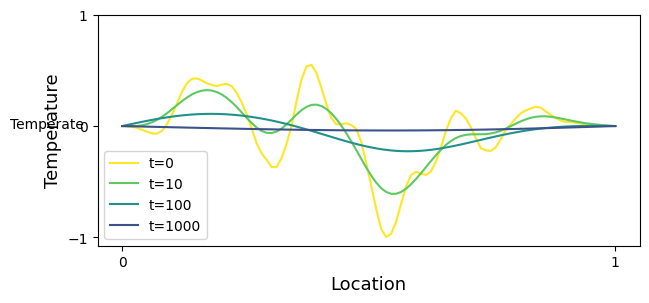
\includegraphics[width=1\columnwidth]{../images/1D_heat.png}
        \captionof{figure}{Numerical solution of the heat equation on $(0,1)\subset \reals$, with Dirichlet BCs $u(0, 0)=u(0, 1)=0$. The solution is shown at four curated timesteps. As time increases, the temperature distribution gets smoother, until it reaches $0$. Since the temperature moves towards the average, and the boundary is fixed at zero, the temperature must go to zero.}
        \label{fig:heat_1d}
    \end{center}
}
\subsection{Method of Lines}
The challenge with ODEs was the continuous parameter $t$, which we overcame by discretizing across the temporal dimension. However, our PDEs now additionally depend on continuous spatial parameters $\mathbf{x}$. The Method of Lines (MOL) \cite{mol} works by converting the PDE to a system of ODEs, for which existing ODE solvers can be used. To convert to a system of ODEs, the only continuous parameter $u$ may depend on is $t$. By discretizing space into finite set of points $\mathbb{X} = (\mathbf{x}_1, \dots, \mathbf{x}_n)$, the continuous spatial input is been reduced to discrete indexing into $n$-vector $u(t)$
$$u(t) = \begin{bmatrix}
    u(t, \mathbf{x}_1), \dots, u(t, \mathbf{x}_n)
\end{bmatrix}^\top$$ 
containing the solution at each of the collocation points. However, having discretized space into a countable set of points, the differential operators acting on the spatial dimension are no longer defined. 

\definition{Collocation points}{
    In finite difference methods, collocation points are the spatial points where the finite difference approximations of derivatives are computed.
}

\definition{Finite Difference Methods}{
    Finite Differences (FD) methods approximate differential operators from finite points of space. Differential operators are defined through limits, but with a finite number of spatial points, the limit must be approximated.
    This yields finite difference operators, which can be applied to functions sampled at the specific points to approximate their spatial derivative.
    \\ 
    Like continuous differential operators, FD operatros are only defined on the interior of the domain. Supplying boundary conditions is therefore still necessary.
}
For linear differential operators the finite difference method will also be linear and can thus be written as a matrix. The exact form of the FD method depends on the discretization. In Euclidean space, rectangular grids yield simple formulas depending on the grid-spacing. On curved manifolds the grid-method breaks down. The methods from Discrete Exterior Calculus (ch. \ref{sec:manifolds}) give formulas for FD operators on discretized manifolds (triangle meshes). 
\example{Finite Differences in One Dimension}{
    In one dimension, from a finite set of collocation points $$\mathbb{X} = (x_1<\dots<x_n<x_{n+1}) \subset (0, 1)$$ one can approximate the first derivative of $u: (0, 1) \to \reals$ on the interior $x_i$ with the central difference 
    $$\frac{\partial}{\partial x}u(x_i) \approx \frac{u(x_{i+1}) - u(x_i)}{x_{i+1} - x_i}$$ 
    This formula is not valid for point $x_{n+1}$ at one end of the boundary. When all points are ordered and equidistant and with distance $h$, this can be expressed as matrix $D\in \reals^{n\times n}$ acting on the vector of samples $\mathbf{u}$:
    $$D\mathbf{u} = \frac{1}{h}
    \begin{bmatrix}
          -1 & 1 & 0 & \dots & \dots & 0
        \\ 0 & -1 & 1 & \ddots & \ddots & \vdots
        \\ \vdots & \ddots & \ddots & \ddots & \ddots & \vdots
        \\ \vdots & \ddots & 0 & -1 & 1 & 0
        \\ 0 & \dots & 0 & 0 & -1 & 1
        \\ 0 & \dots & 0 & 0 & 0 & -1
    \end{bmatrix}\begin{pmatrix}u(x_1) \\ \vdots \\ u(x_n)\end{pmatrix}$$ The final row is not defined TODO CHECK THE USUAL FORMULAS
}
\example{Finite Differences, Laplacian}{
    To approximate the second derivative, one can simply apply the first derivative twice. The matrix $D^2$ will then be the matrix product $D\cdot D$, with shape 
    $$D^2 = \begin{bmatrix} 1 & -2 & 1 & 0 & \dots & 0 \\ 0 & 1 & -2 & 1 & \dots & 0 \\ \vdots & \vdots & \vdots & \vdots & \ddots & \vdots \\ 0 & 0 & 0 & 0 & \dots & 1\end{bmatrix}$$ 
    TODO CHECK DIMENSIONS. TODO CHECK 
}
\example{Method of Lines applied to the Heat Equation}{
    The heat equation (\ref{eq:heat_equation}) makes use the linear differential operator $\Delta$, the Laplacian. By discretizing into spatial points $n = |\mathbb{X}|$ and deriving a suitable matrix $L\in\reals^{n\times n}$ estimating $\Delta$, we get the system of $n$ ODEs
    $$\hspace*{-3mm}i\!\in\!\{1,.., n\}\!: \hspace{2mm} \frac{d}{dt}u(t)_i = -L_i u(t)  \in \reals \hspace{14mm}$$
    where $L_i$ the $i$th row of $L$.
    We can write it more eloquently in vector-form by stacking all the spatial points to get
    \begin{align}\label{eq:space_stack}
        \frac{d}{dt}u(t) = -L u(t) \in \reals^n
    \end{align}
    \\
    The solution in figure \ref{fig:heat_1d} was obtained using this exact method, for $\mathbb{X} = \{0, \frac{1}{100}, \frac{2}{100}, \dots, \frac{99}{100}, 1\}$ and the FD Laplacian matrix from the previous box.
}
\algorithmbox{!!!Key Insight!!!}{
    Note that, once the differential operator is discretized, there is no reference to the underlying metric or topological structure. This information is encoded exclusively in the differential operator.
}
\example{Method of Lines applied to the Wave Equation}{
    The wave equation describes the evolution of the height of a wave $u(t, \mathbf{x})$ at a point $\mathbf{x}$ and time $t$.
    \begin{align}\label{eq:heat_equation}
        \frac{\partial^2}{\partial t^2}u = -\Delta u
    \end{align}
    Here, the vector field now prescribes the second-time derivative of $u$. We proceed with the Method of Lines:
    \\ Discretize space into $n = |\mathbb{X}|$ spatial points, compute matrix $L$ approximating $\Delta$. Similarly to the heat equation, we end up with the system of $n$ $2$nd order ODEs 
    $$\frac{d^2}{dt^2}u(t) = -L u(t) \in \reals^n$$
    As we prefer feeding $1$st order ODEs to our solvers, we will convert our $n$ second order ODEs to $2n$ first-order ODEs with the stacking equation (\ref{eq:stack})
    $$\frac{d}{dt}\vec{u} = \frac{d}{dt} \begin{pmatrix}
        u \\ v
    \end{pmatrix}= \begin{pmatrix}
        v \\ -L u
    \end{pmatrix}
    \in \reals^{2n}
    $$
    By linearity of $L$ we now apply the idea of eq. \ref{eq:linear_stack} to write everything as a single system matrix
    $$= \begin{bmatrix}
        \textbf{0} & \text{I}_n \\ -L & \textbf{0}
    \end{bmatrix} \begin{pmatrix}
        u \\ v
    \end{pmatrix} = A \vec{u_i}
    $$
    A is of dimension $2n \times 2n$ but highly sparse. The identity matrix $\text{I}_n$ plays the same role as the "$1$" in eq. \ref{eq:linear_stack}.
}
The sparse of these high order system matrices will play a big part in later section where we will specify prior distributions over PDE solutions. For good measure, we will take a few more examples of linear PDEs and give their resulting system matrix.

\example{MOL on different PDEs and their 1st Order ODE Representation}{
    In the following table, $\textbf{I}$ is the $n\times n$ identity matrix, and $\mathbf{0}$ the $n\times n$ zero matrix.
    \begin{tabular}{c|c}
        \hline 
        Linear PDE & MOL Vector Field
        \\\hline \hspace*{2mm} & \hspace*{2mm} 
        % START
        \\$\frac{\partial}{\partial t}u = -\Delta u$ & $\begin{bmatrix}
            -L
        \end{bmatrix} \begin{pmatrix}
            u
        \end{pmatrix}$
        \\ \hspace*{2mm} & \hspace*{2mm} 
        % END
        
        % START
        \\\hline \hspace*{2mm} & \hspace*{2mm} 
        \\$\frac{\partial^2}{\partial t^2}u = ku  -d\Delta \frac{\partial}{\partial t}u$ & $\begin{bmatrix}
            \textbf{0} & \textbf{I} \\ k\textbf{I} & -dL
        \end{bmatrix} \begin{pmatrix}
            u \\ v
        \end{pmatrix}$
        \\ \hspace*{2mm} & \hspace*{2mm} 
        % END
        
        % START
        \\\hline \hspace*{2mm} & \hspace*{2mm} 
        \\$\frac{\partial^2}{\partial t^2}u = a\Delta \frac{\partial}{\partial t}u$ & 
        $\begin{bmatrix}
            \textbf{0} & \textbf{I} 
            \\ \textbf{0} & aL
        \end{bmatrix} 
        \begin{pmatrix}
            u \\ v
        \end{pmatrix}$
        \\ \hspace*{2mm} & \hspace*{2mm} 
        % END

        % START
        \\\hline \hspace*{2mm} & \hspace*{2mm} 
        \\$\frac{\partial^3}{\partial t^3}u = \Delta u$ & 
        $\begin{bmatrix}
            \textbf{0} & \textbf{I} & \textbf{0}
            \\\textbf{0} & \textbf{0} & \textbf{I}
            \\ L & \textbf{0} & \textbf{0}
        \end{bmatrix} 
        \begin{pmatrix}
            u \\ v_1 \\ v_2
        \end{pmatrix}$
        \\ \hspace*{2mm} & \hspace*{2mm} 
        % END
        % START
        \\\hline \hspace*{2mm} & \hspace*{2mm} 
        \\$\frac{\partial^4}{\partial t^4}u = \Delta u + a\frac{\partial^2}{\partial t^2}u $ & 
        $\begin{bmatrix}
            \textbf{0} & \textbf{I} & \textbf{0} & \textbf{0}
            \\\textbf{0} & \textbf{0} & \textbf{I} & \textbf{0}
            \\ \textbf{0} & \textbf{0} & \textbf{0} & \textbf{I}
            \\ L & \textbf{0} & \!\!a\textbf{I} \!\!& \textbf{0}
        \end{bmatrix} \!
        \begin{pmatrix}
            u \\ v_1 \\ v_2
        \end{pmatrix}$
        \\ \hspace*{2mm} & \hspace*{2mm} 
        % END
    \end{tabular}
    \\
    \\
    Notice the presence of the off-diagonal series of $\textbf{I}$. For an order $q$ PDE (or ODE), the upper 
}\noindent
Approximating the spatial derivatives is a simplified model, which is a source of error. The Probabilistic Numerical Solution in this thesis only models the error from time-discretization.
\example{Error Introduced by Spatial Discretization}{
    The Method of Lines proceeds in two independent steps, spatial discretization and temporal discretization. The way these two steps introduce approximation error are however \textit{not} independent. The error from a coarse spatial resolution can not be alleviated by arbitrarily increasing the temporal resolution and vice-versa. In \cite{pnmol} the authors propose the \textit{Probabilistic Numerical Method of Lines}, which quantifies the discretization error with probabilistic finite-difference methods. TODO Yes?
}

\ifdefined\COMPILINGFROMMAIN
\else    
    \end{document}
\fi

\clearpage
\section{Probabilistic Numerical Solver for ODEs}\label{sec:prior}
\ifdefined\COMPILINGFROMMAIN
\else
    %%%%HEADER
\documentclass[twocolumn]{article}
\usepackage[a4paper, margin=1in, columnsep=20pt]{geometry}
\usepackage{amsmath, amssymb, graphicx, hyperref}
\usepackage[most,skins,breakable]{tcolorbox}
\usepackage[symbol]{footmisc}
\usetikzlibrary{calc}
\usepackage{xcolor}
\usepackage{caption}
\usepackage{algorithm}
\usepackage{algpseudocodex}
\usepackage{tikz}
\usepackage{listings}
\usetikzlibrary{arrows.meta, positioning}
\tcbuselibrary{listingsutf8}
\usepackage{microtype}
\usepackage{blindtext}
\usepackage{bookmark}
\usepackage{breqn}
\usepackage[backend=biber,style=numeric]{biblatex} % 
\addbibresource{../references.bib}

% Define style for the listings environment
\lstdefinestyle{mystyle}{
    basicstyle=\ttfamily\small,
    breaklines=true,
    escapeinside={(*@}{@*)}, % Allows math mode within listings
    numbers=left,
    numberstyle=\tiny,
    frame=single,
    keywordstyle=\color{blue}\bfseries,
    commentstyle=\color{green!50!black},
    stringstyle=\color{red}
}


\def\reals{\mathbb{R}}
% Define the custom definition box and command
\newtcolorbox{mydefinition}[2][]{%
    text width=0.95\columnwidth,
    before=\vspace{1mm}, 
    after=\vspace{1mm}, 
    colback=gray!10, % Background color (light gray)
    colframe=black!70,  % Border color
    coltitle=gray!10,  % Title color
    fonttitle=\bfseries, % Title font style
    sharp corners,   % Box style
    left=2pt,
    breakable,
    right=2pt,
    top=2pt,
    bottom=2pt,
    enhanced jigsaw,
    title=Definition: {#1},         % Title passed as the first argument
    colupper=black,  % Ensure proper content handling
    pad at break*=1pc,
    overlay first and middle={
        \coordinate (A1) at ($(interior.south east) + (-10pt,5pt)$);
        \coordinate (C1) at ($(interior.south east) + (-6pt,7.5pt)$);
        \draw[fill=black!50] (A1) -- +(0,5pt) -- (C1) -- cycle;
    }
    }
    
\newcommand{\definition}[2]{%
    \noindent%
    \begin{mydefinition}[#1]%
        .#2%
    \end{mydefinition}%
    \noindent
}

\newtcolorbox{myexample}[2][]{%
    text width=0.95\columnwidth,
    before=\vspace{1mm}, 
    after=\vspace{1mm}, 
    colback=orange!3, % Background color (light gray)
    colframe=black!70,  % Border color
    coltitle=gray!10,  % Title color
    fonttitle=\bfseries, % Title font style
    sharp corners,   % Box style
    left=2pt,
    right=2pt,
    top=2pt,
    bottom=2pt,
    breakable,
    title=Intuition: {#1},         % Title passed as the first argument
    pad at break*=1pc,
    overlay first and middle={
        \coordinate (A1) at ($(interior.south east) + (-10pt,5pt)$);
        \coordinate (C1) at ($(interior.south east) + (-6pt,7.5pt)$);
        \draw[fill=black!50] (A1) -- +(0,5pt) -- (C1) -- cycle;
    }
}

\newcommand{\example}[2]{%
    \noindent%
    \begin{myexample}[#1]%
    .#2%
    \end{myexample}%
    \noindent
}

\newtcolorbox{algobox}[2][]{%
    text width=0.95\columnwidth,
    before=\vspace{1mm}, 
    after=\vspace{1mm}, 
    colback=blue!5, % Background color (light gray)
    colframe=black!70,  % Border color
    coltitle=gray!10,  % Title color
    fonttitle=\bfseries, % Title font style
    sharp corners,   % Box style
    left=2pt,
    right=2pt,
    top=2pt,
    bottom=2pt,
    breakable,
    title=Algorithm: {#1},         % Title passed as the first argument
    pad at break*=1pc,
    overlay first and middle={
        \coordinate (A1) at ($(interior.south east) + (-10pt,5pt)$);
        \coordinate (C1) at ($(interior.south east) + (-6pt,7.5pt)$);
        \draw[fill=black!50] (A1) -- +(0,5pt) -- (C1) -- cycle;
    }
}

\newcommand{\algorithmbox}[2]{%
\noindent%
    \begin{algobox}[#1]%
    .#2%
    \end{algobox}%
    \noindent
}
%%%%HEADER

    \begin{document}
\fi


\section*{Probabilistic Numerical Solvers for ODEs}
A probabilistic numerical (PN) solver of ODEs is fundamentally different than a classic numerical solver.
A PN starts with a prior distribution over solutions of the solution function $u$, which is then conditioned on information about the vector field $f$. The resulting posterior distribution is referred to as a PN solution of the ODE \cite{nicoThesis}.
We will go through the different steps and cover the prerequisites.

\subsection*{Specifying a Prior Distribution}
Prior distributions over functions are a natural way to model uncertainty in the solution of an ODE. We are interested in tractable computation of the later posterior, which limits our choice of prior. Our prior distribution should be a distribution over functions that is easy to sample from and easy to condition on information. We will focus on the class of Gauss-Markov (\cite{gp_Rasmussen}) processes, which are a Gaussian processes that additionally have the Markov property.
\definition{Markov Property}{
    A stochastic process $U$ has the Markov property if for all $i < s < t$ $$U(t) \perp U(i) \;|\; U(s)$$
    In words, the future is independent of the past given the present. The state at time $t$ must therefore contain all relevant information about the past.
}
In particular, we will use a Gauss-Markov prior for the full state-space representation of $u$, containing $u$ and its first $q\geq 1$ time-derivatives. 
$$\vec{U} :=\begin{bmatrix} U & \frac{d}{d t} U & \cdots & \frac{d^q}{d t^q} U\end{bmatrix}^{\top} \sim \mathcal{GP}$$

\subsubsection*{Linear Time-Invariant Stochastic Differential Equation}
Linear TI SDEs are a class of SDEs that are linear in the state and the noise, and whose system matrices do not depend on the current time.
\definition{Linear Time-Invariant Stochastic Differential Equation}{
    A linear SDE can be written in the form
    \begin{align}\label{eq:LSDE_definition}
        dX(t) = F X(t) dt + L dW(t)
    \end{align}
    where $X(t)\in \reals^n$ is the state, $F\in \reals^{n \times n}$ is the system matrix, $L\in \reals^{n \times n}$ is the diffusion matrix, and $W(t)\in \reals^n$ is a Wiener process. This is known as the Itô form of the SDE. The solution of the SDE is a stochastic process $X(t)$ (\cite{sde-book}).
}
They are a simple choice for the dynamics of the state-space representation of the solution function $u$ and have closed form solutions for the posterior distribution.
\example{Motivating Linear SDEs}{
    A linear SDE can be obtained by injecting gaussian noise into a deterministic ODE. If we start off with the harmonic oscillator with an external force $f(t)$
    $$\frac{d^2}{dt^2}u = -ku - l\frac{d}{dt}u + f(t)$$
    If we do not know the external force and believe it to be independent of previous terms, we might model it as a gaussian noise term $\xi(t) \sim \mathcal{N}(0, \sigma^2)$, giving the linear SDE
    $$\frac{d^2}{dt^2}U = -kU - l\frac{d}{dt}U + \xi(t)$$
    This states that the second derivative is a combination of the first derivative and the function itself, plus noise. The noise makes the system stochastic, hence the capital $U$ notation. TODO SUS However, the noise is nowhere differentiable, and so the expression $\frac{d^2}{dt^2}U$ is not defined. We avoid this issue by combining the SDE notation with a state-space representation of $U$ as $\vec{U} = [U \; \frac{d}{dt}U]^\top$
    $$d\vec{U} = \begin{bmatrix} 0 & 1 \\ -k & -l \end{bmatrix} \vec{U} dt + \begin{bmatrix} 0 & 0 \\ 0 & \sigma \end{bmatrix} dW(t)$$
    Below is shown this spring model. The initial distribution of the state is chosen as $$\vec{U}(0) \sim \mathcal{N}([1, 0]^\top, \text{diag}([0.2^2, 0.1^2]))$$
    \begin{center}
        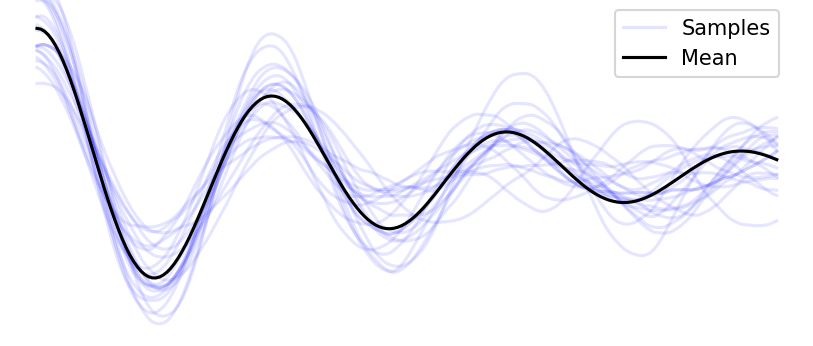
\includegraphics[width=\columnwidth]{../images/stochastic_spring_samples.png}
        \captionof{figure}{50 samples from the linear SDE describing the stochastic spring model with random independent force. The random force has $\sigma = 0.1$ and we have $k=1$, $l=0.2$.}
    \end{center}
}
\newpage
\definition{Integrated Wiener Process}{
    \begin{center}
        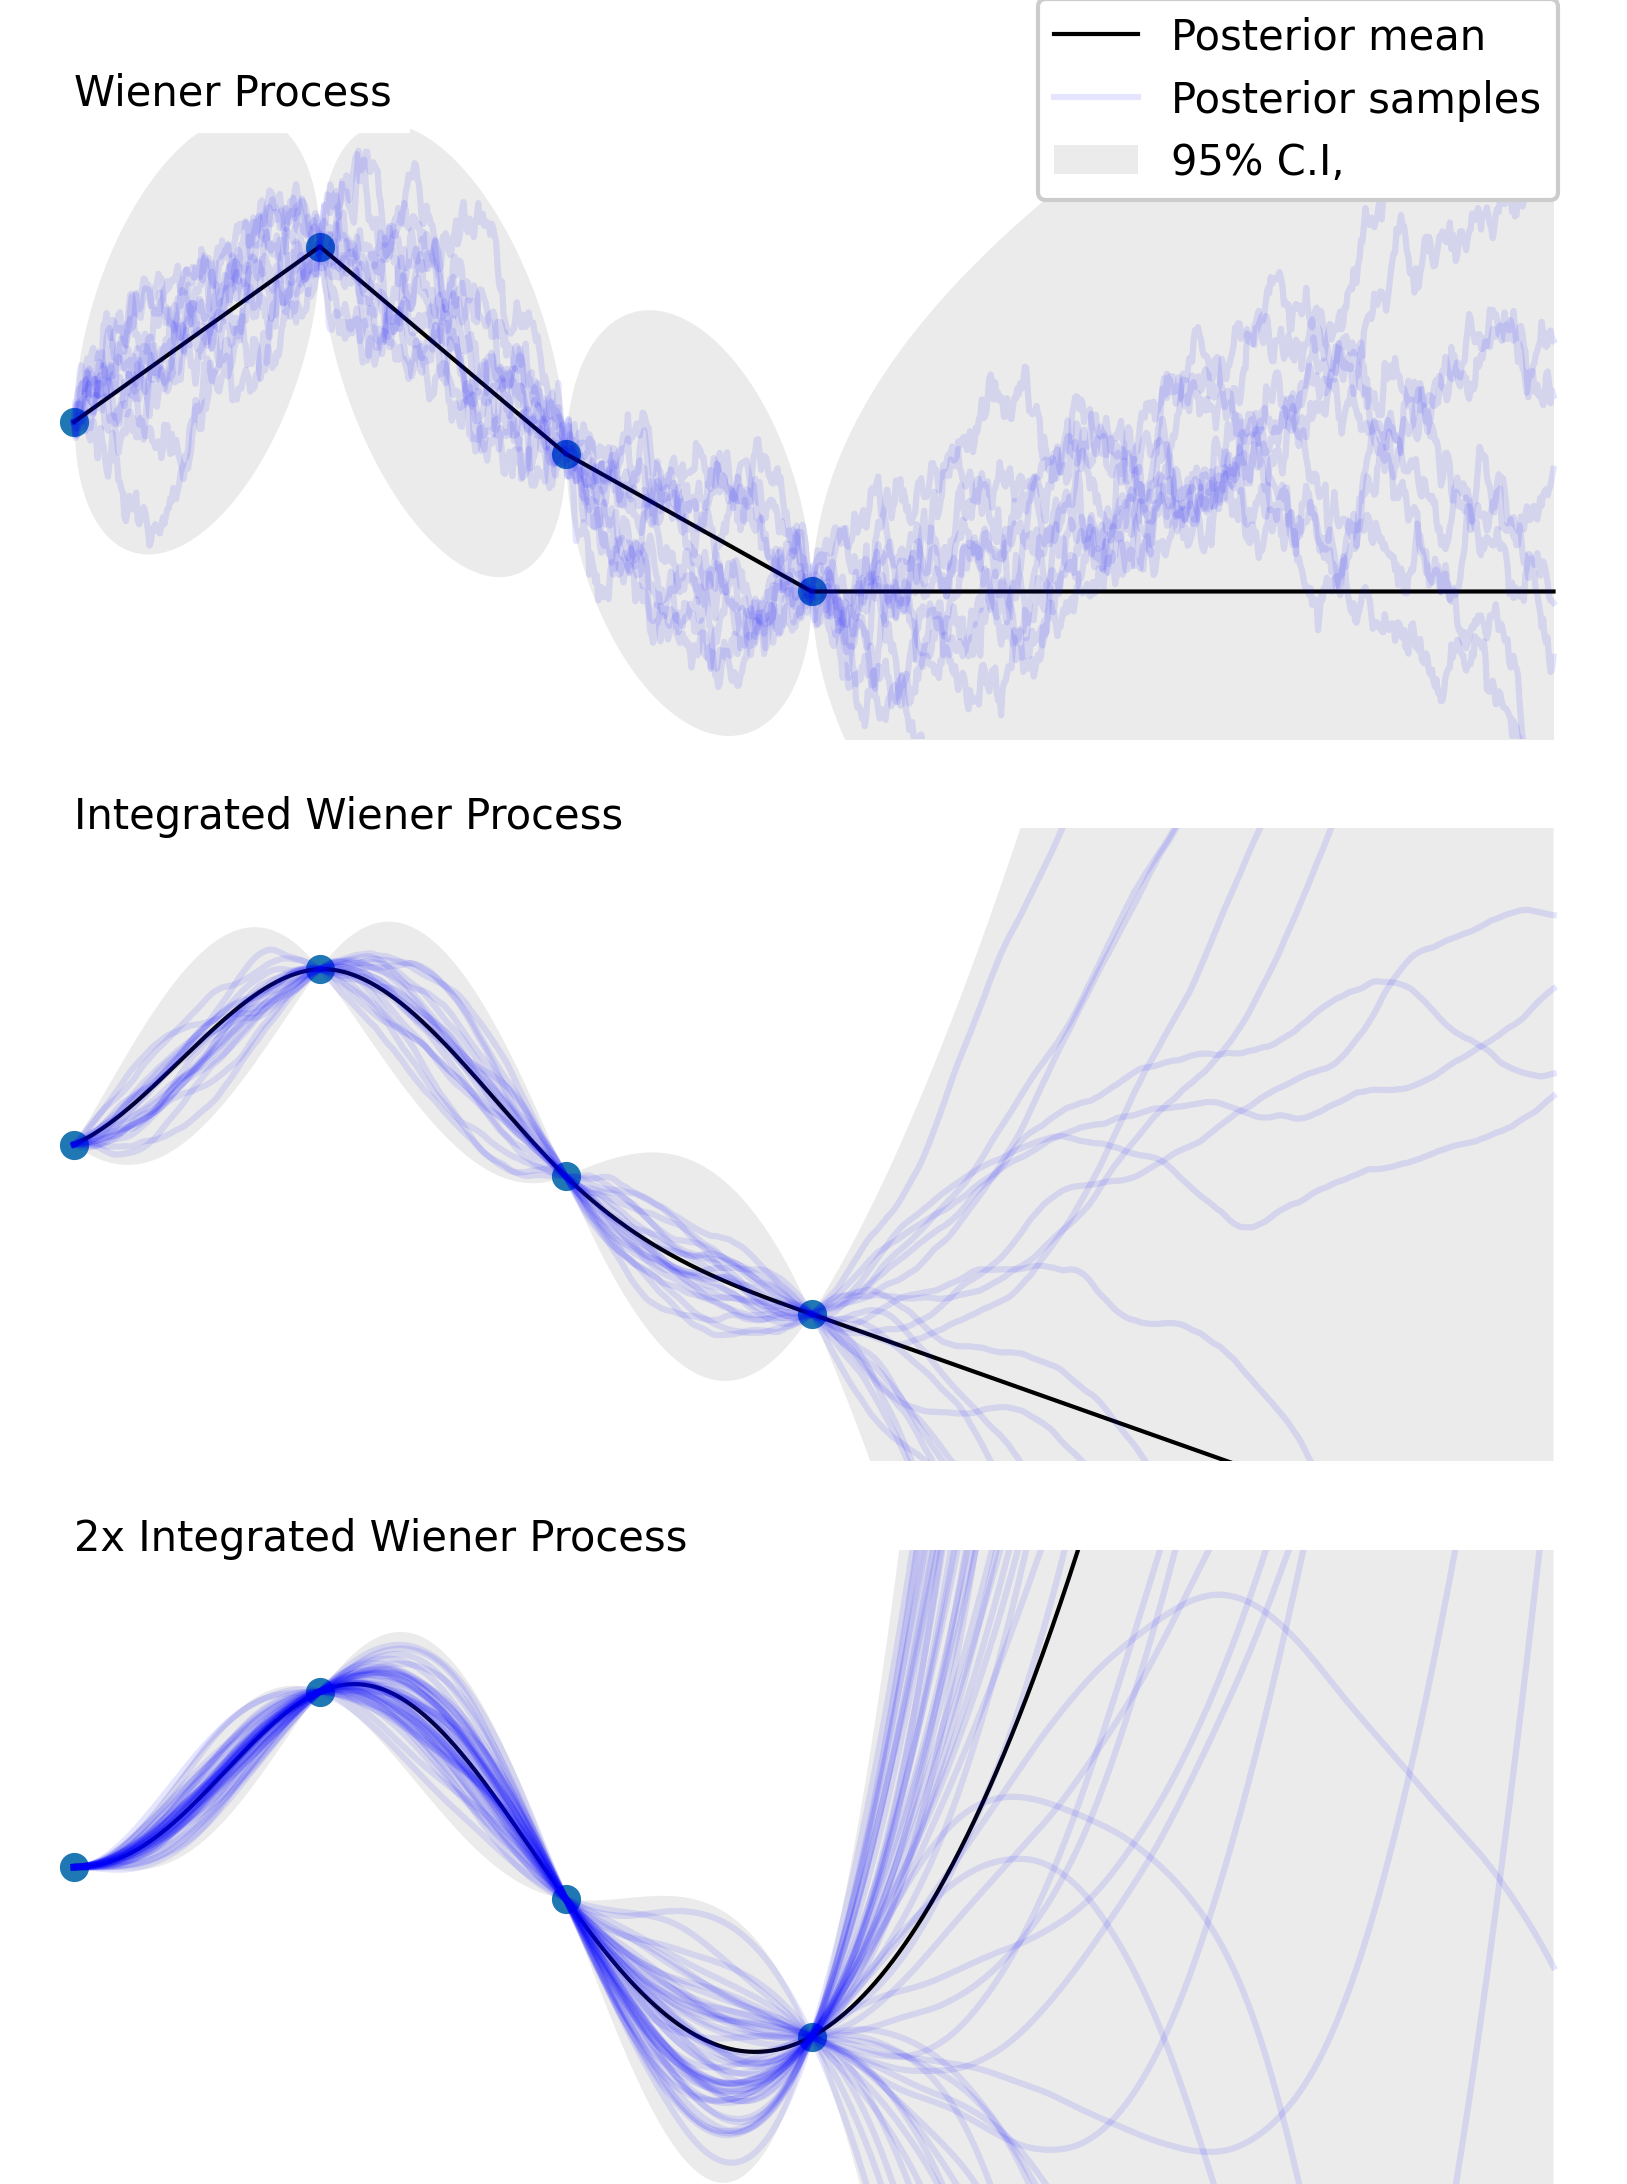
\includegraphics[width=\columnwidth]{../images/conditioned_iwps.png}
        \captionof{figure}{Three graphs of the [x-Integrated] Wiener Process. The processes are conditioned to pass through four different points, marked in blue, the derivative is however unspecified.}
        \label{fig:iwps}
    \end{center}
    The Wiener Process, also known as Brownian motion, is continuous but nowhere differentiable. In terms of eq. \ref{eq:LSDE_definition} its state-space representation is 1-dimensional with $$F=0  \hspace{1cm}L=1$$ 
    The Integrated Wiener Process is the integral of the Wiener Process. The state-space representation is 2-dimensional with $$F=\begin{bmatrix}
        0 & 1 \\ 0 & 0
    \end{bmatrix} \hspace{1cm} L=\begin{bmatrix}
        0 & 0 \\ 
        0 & 1 
    \end{bmatrix}$$
    \\ The Twice Integrated Wiener Process has 3-dimensional state-space with $$F=\begin{bmatrix}
        0 & 1 & 0 \\ 0 & 0 & 1 \\ 0 & 0 & 0
    \end{bmatrix} \hspace{1cm} L=\begin{bmatrix}
        0 & 0 & 0 \\ 0 & 0 & 0 \\ 0 & 0 & 1
    \end{bmatrix}$$
    \\ The posterior means of the $q$-times integrated Wiener process are 2q + 1-ic splines (\cite{probnum}) - see the figure above. There is in principle nothing preventing us from using higher order integrated Wiener processes, but numerical issues are encountered at around $q=3$. We will tackle this later.
}
\newpage
\definition{Ornstein Uhlenbeck Process}{
    \begin{center}
        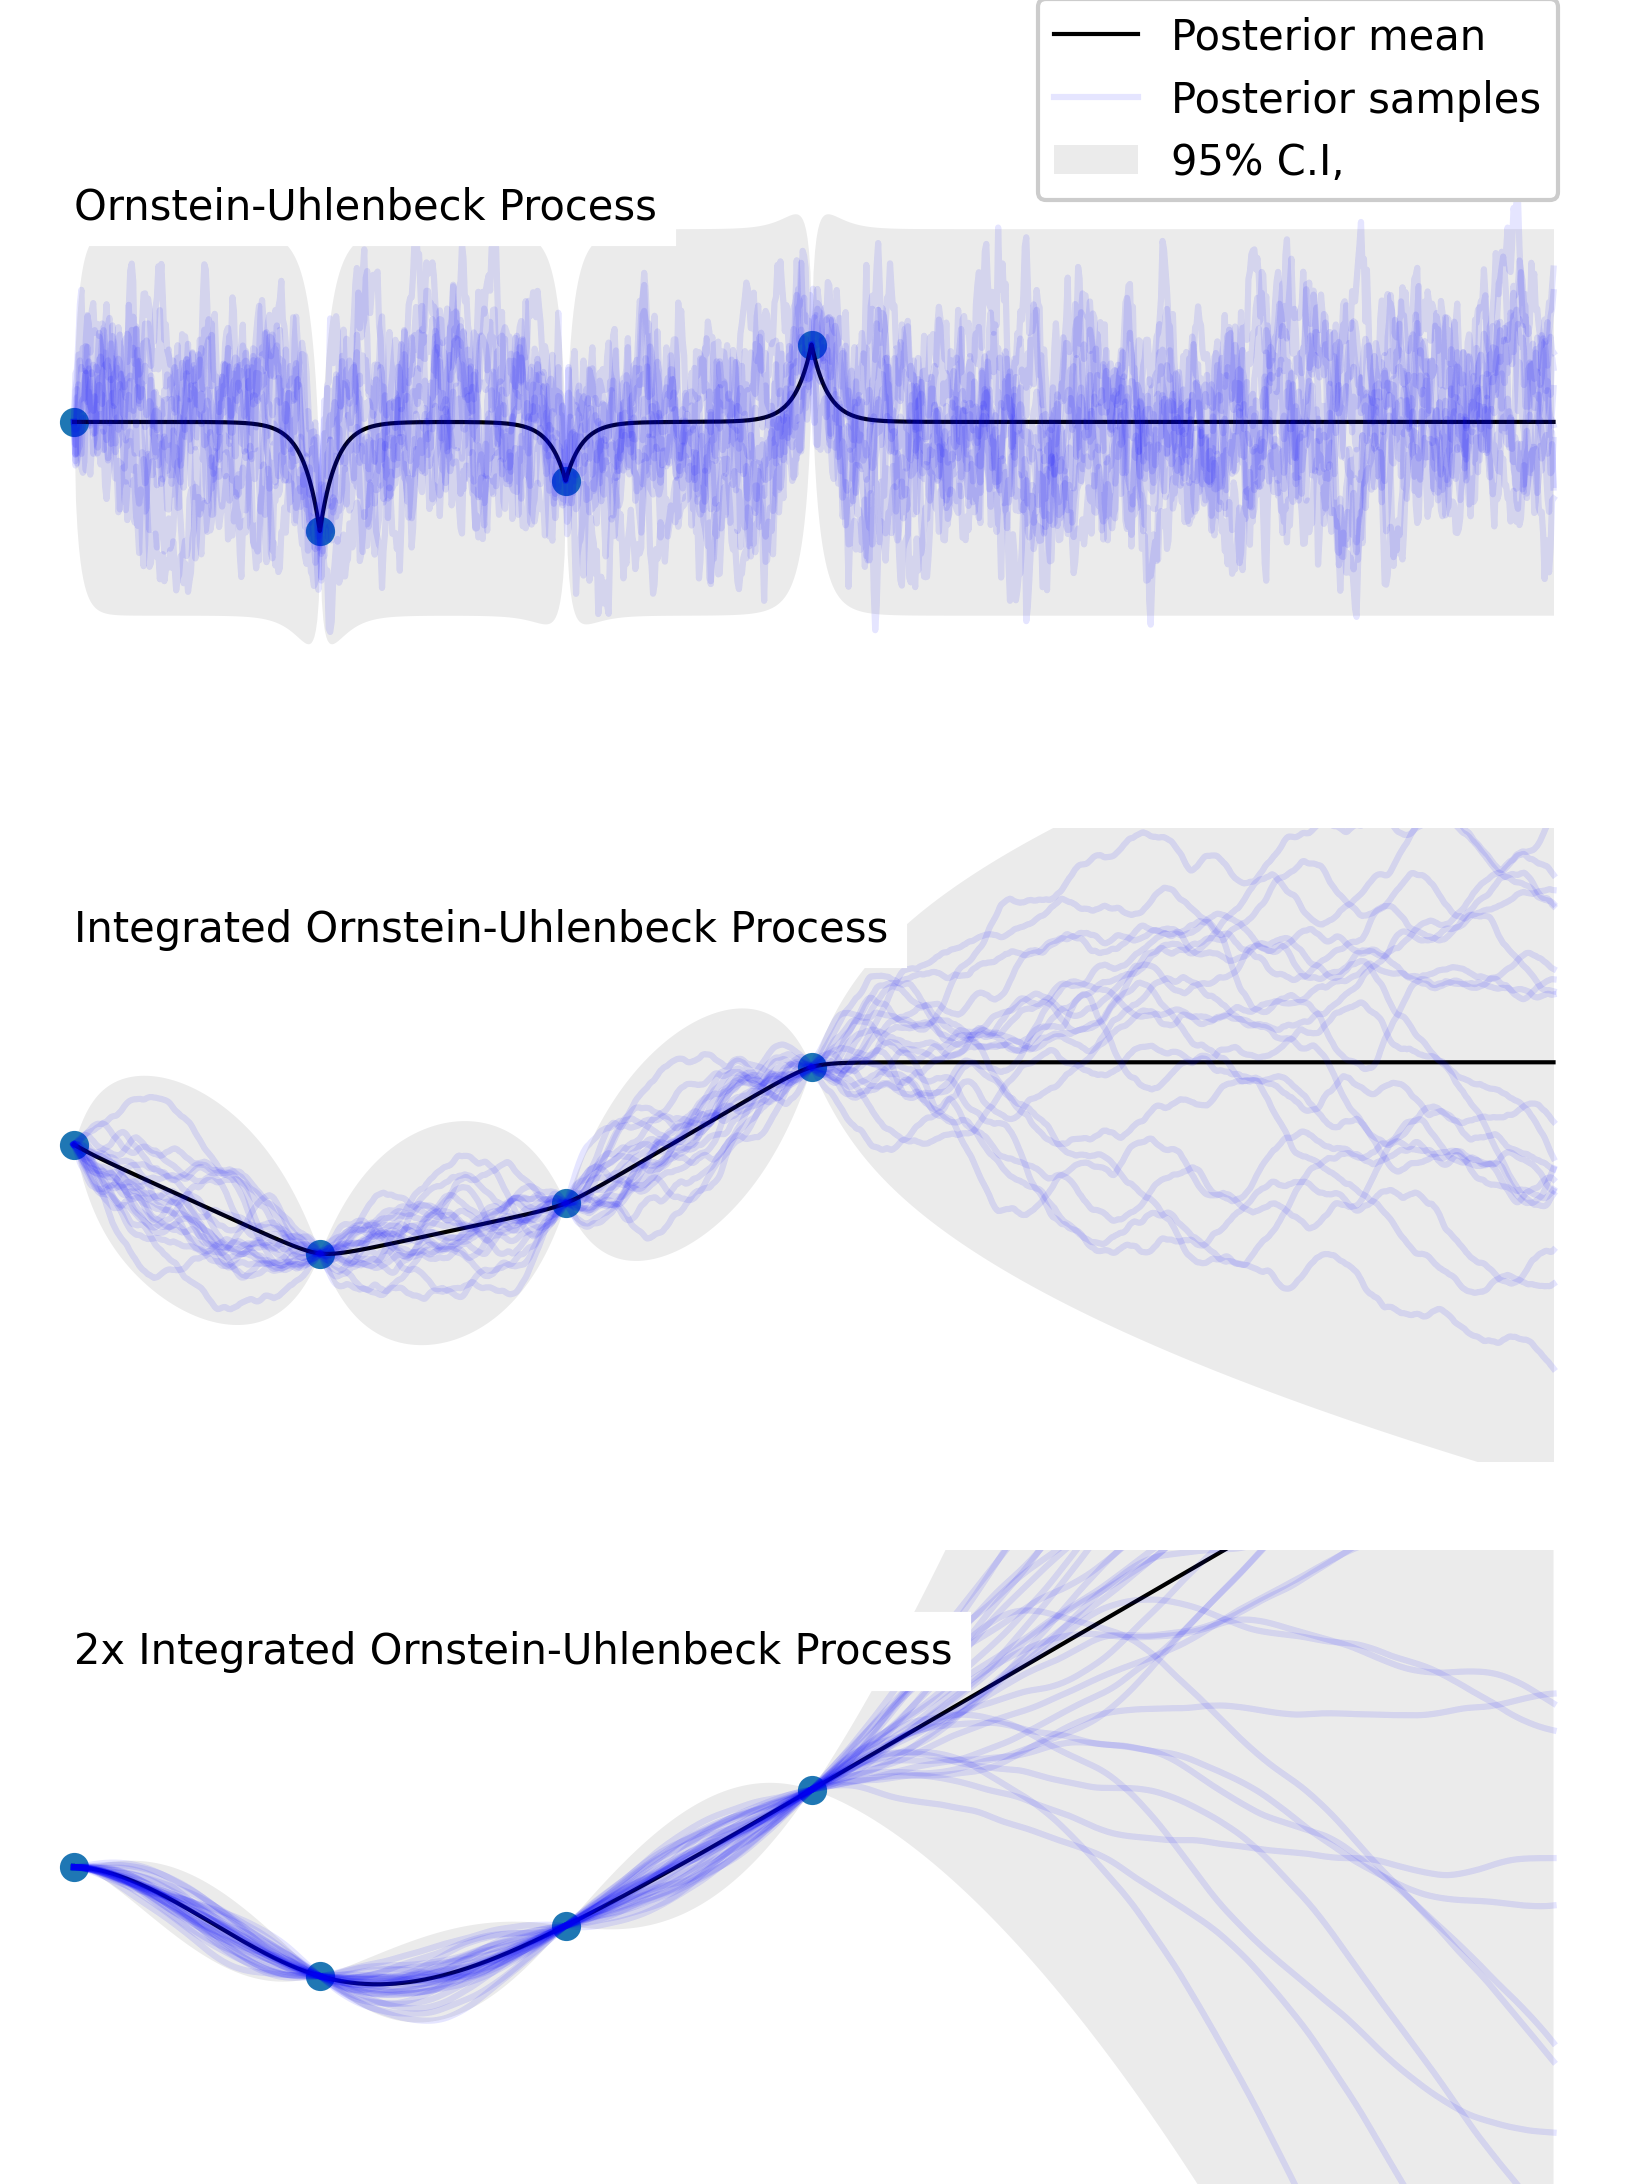
\includegraphics[width=\columnwidth]{../images/conditioned_ous.png}
        \captionof{figure}{Draws from the Integrated Wiener Process, Conditioned}
    \end{center}
    The Ornstein-Uhlenbeck Process depends on rate parameter $a>0$. In terms of eq. \ref{eq:LSDE_definition} its state-space representation is 1-dimensional with $$F=-a  \hspace{1cm}L=1$$ 
    The Integrated Ornstein-Uhlenbeck is the integral of the Ornstein-Uhlenbeck. The state-space representation is 2-dimensional with $$F=\begin{bmatrix}
        0 & 1 \\ 0 & -a
    \end{bmatrix} \hspace{1cm} L=\begin{bmatrix}
        0 & 0 \\ 0 & 1
    \end{bmatrix}$$
    \\ The Twice Integrated Ornstein-Uhlenbeck has 3-dimensional state-space with $$F=\begin{bmatrix}
        0 & 1 & 0 \\ 0 & 0 & 1 \\ 0 & 0 & -a
    \end{bmatrix} \hspace{1cm} L=\begin{bmatrix}
        0 & 0 & 0 \\ 0 & 0 & 0 \\ 0 & 0 & 1
    \end{bmatrix}$$
    In \cite{exponential_probabilistic} they suggest using the Ornstein-Uhlenbeck process to encode prior information to solve particularly difficult "stiff" DEs.\\
    The Ornstein-Uhlenbeck process is mean-reverting (\cite{probnum}), the derivative of the Integrated Ornstein-Uhlenbeck reverts to zero, and the curvature of the Twice Integrated Ornstein-Uhlenbeck reverts to zero.
}
\example{Encoding Prior Dynamics: Wave Process}{
\begin{center}
    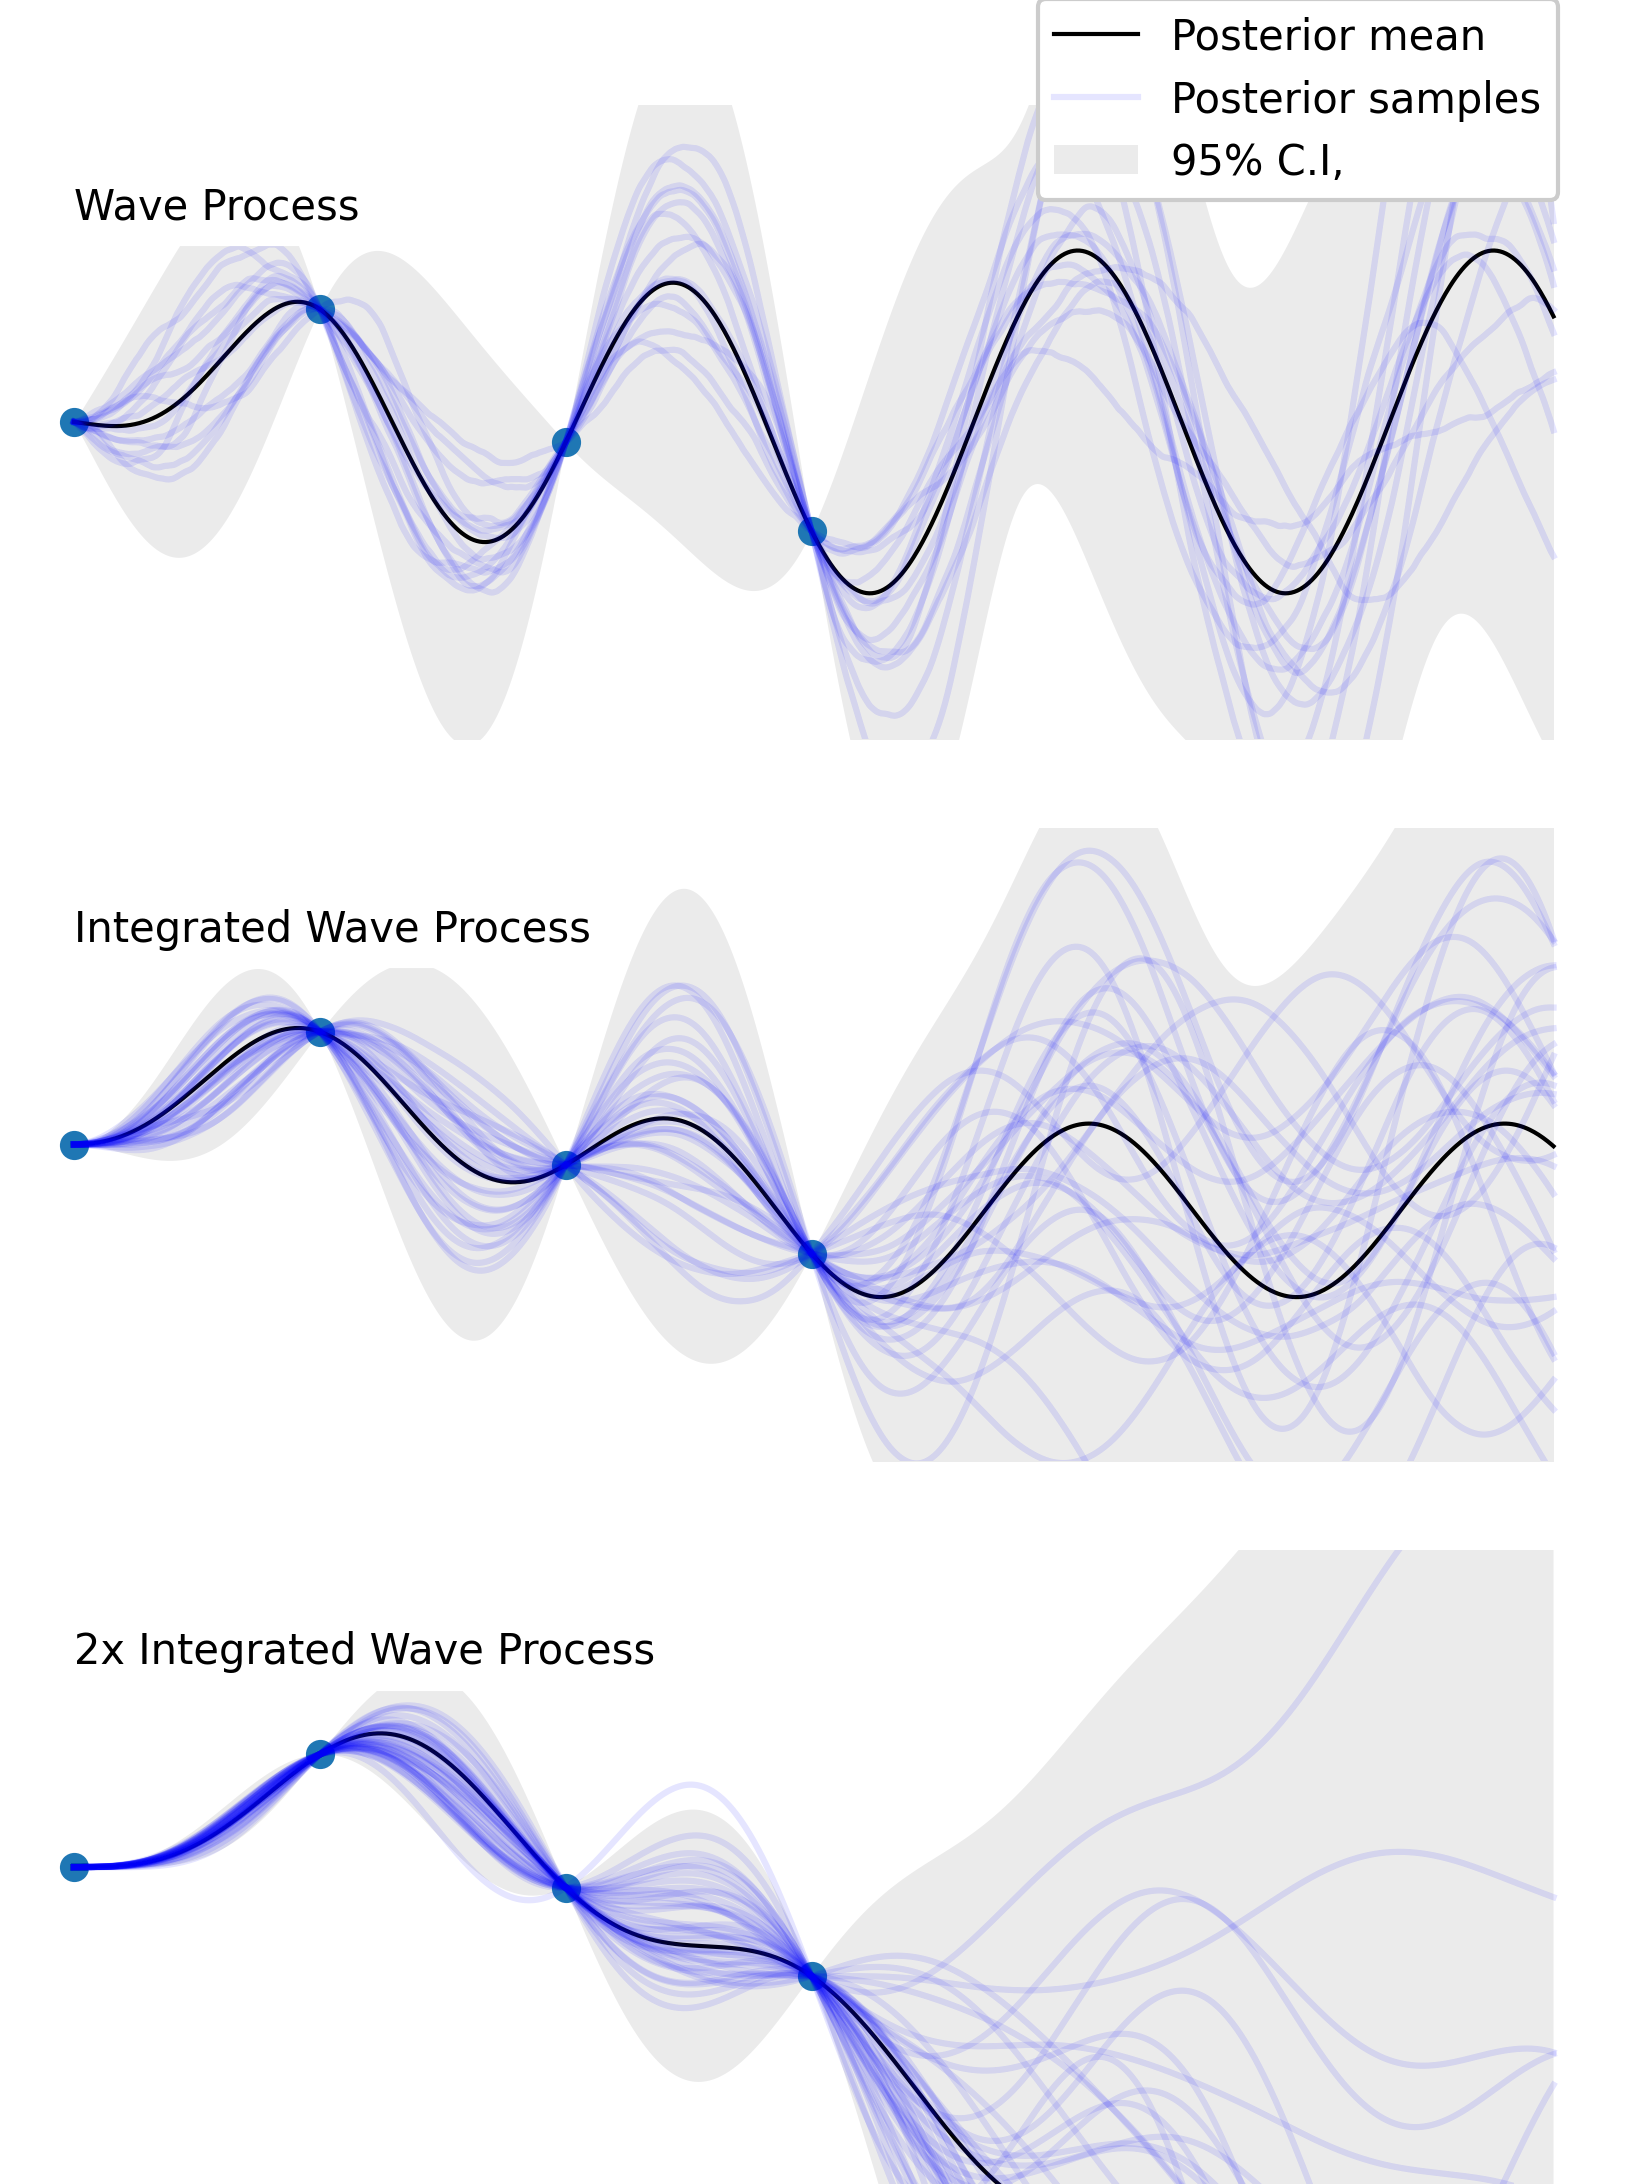
\includegraphics[width=\columnwidth]{../images/conditioned_waves.png}
    \captionof{figure}{Draws from the Integrated Wiener Process, Conditioned}
\end{center}
}


\subsection*{Solving LTI Stochastic Differential Equations}
If the initial distribution is gaussian (which includes a deterministic initial condition) the distribution of a linear SDE can be expresed in closed form. At each time, it will be a multivariate gaussian. For the linear SDE \ref{eq:LSDE_definition}, the following holds
\begin{align}\label{eq:SDE_mean}
    \mathbb{E}[X(t)] = e^{At}\mathbb{E}[X(0)]
\end{align}
Which means, that in expectation the will satisfy the differential equation exactly. This is essentially the same expression as the analytical solution to a deterministic ODE. The covariance matrix of the state at time $t$ is given by
\begin{align}\label{eq:SDE_cov}
    \text{Cov}[X(t)] = \int_0^t e^{A(t-s)}BB^\top e^{A^\top(t-s)} ds
\end{align} TODO CHECK THIS


\subsection*{Discretizing the Prior in Time}
Similarly to the Method Of Lines, we now consider a finite set of times $\mathbb{T} = \{h, 2h, 3h, \dots, T\}$, where $h$ is the timestep size and $T$ is the final time. For simplicity, we choose a fixed timestep, but it can be heterogenous or even adaptive, see \cite{nicoThesis}. 
\\
The Markov property enables the discrete time stochastic recurrence relation (\cite{probnum}) using eq. \ref{eq:SDE_mean} and \ref{eq:SDE_cov}
\begin{align}\label{eq:discrete_time_recurrence}
    \vec{U}(t+h) \;|\; \vec{u}(t) \sim \mathcal{N}(A\vec{u}(t), Q)
\end{align}
with discrete-time transition matrices
\begin{align}
    A &= e^{Fh}\label{eq:easy_matrix_exponential}
    \\
    Q &= \int_0^h e^{Ft}LL^\top e^{F^\top t} dt \label{eq:hard_matrix_exponential}
\end{align}
The formula \ref{eq:easy_matrix_exponential} can be computed numerically quite simply with JAX \cite{jax} or other numerical linear algebra libraries. \ref{eq:hard_matrix_exponential} is however quite difficult, but using Matrix Fraction Decomposition it too can be reduced to a matrix exponential.
\definition{Matrix Fraction Decomposition}{
    The following algorithm for $A$ and $Q$ is originally from \cite{sde-book} but simplified for our fixed-time-step and time-invariant. We will use their notation.
    \\
    Assume the SDE to be discretized is of the form
    $$dX(t) = FX(t)dt + L dW(t)$$ with $F, L \in \reals^{n\times n}$. Compute the matrix exponential of the block-matrix as $M$
    $$M =\exp{\left(h\begin{bmatrix}
        F & L \\ 0 & -F^\top
    \end{bmatrix}\right)}$$
    Extract the upper left block of $M$ as $A\in\reals^{n\times n}$ and the upper right as $C \in \reals^{n\times n}$. Finally, compute $Q$ as $Q = CA^\top$.
}
We can now form the conditional distribution of the state at each time given the state at the previous time. For brevity, we will from here on refer to as the finite-time states $\vec{U}(i\cdot h)$ with an integer subscript index $\vec{U}_i$.When combining the conditonal distribution \ref{eq:discrete_time_recurrence} with an initial gaussian distribution 
$$\vec{U}_0 \sim \mathcal{N}(\mu_0, \Sigma_0)$$ 
we can form the factorized joint distribution of the process across all discrete times as 
$$P(\vec{u}_{\mathbb{T}}) = P(\vec{u}_0, \vec{u}_1, \dots, \vec{u}_{|T|}) =$$
$$\mathcal{N}\Big(\vec{u}_0;\;\mu_0, \Sigma_0\Big)\prod_{t=1}^{|\mathbb{T}|} \mathcal{N}\Big(\vec{u}_t;\;A\vec{u}_{t-1}, Q\Big)$$
This is an instance of a Linear Gaussian Model, which is a tractable and chain-structured bayesian network, depicted below.
\begin{center}
    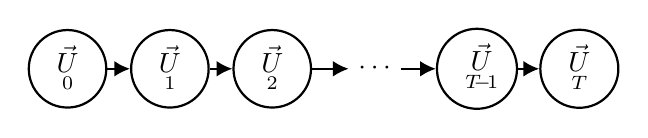
\begin{tikzpicture}[node distance=1.3cm, >={Latex[length=2mm, width=2mm]}, 
        obs/.style={circle, draw, align=center, text width = 3mm, minimum size=3mm, thick, font=\sffamily},
        lat/.style={rectangle, draw, align=center, text width = 6mm, minimum size=6mm, thick, font=\sffamily}]
        
        % Nodes
        \node[obs] (U0) {$\underset{0}{\vec{U}}$};
        \node[obs, right of=U0] (U1) {$\underset{1}{\vec{U}}$};
        \node[obs, right of=U1] (U2) {$\underset{2}{\vec{U}}$};
        \node[right of=U2] (dots) {$\cdots$};
        \node[obs, right of=dots] (UTb) {$\underset{T\!\!-\!1}{\vec{U}}$};
        \node[obs, right of=UTb] (UT) {$\underset{T}{\vec{U}}$};
        
        % Edges
        \draw[->, thick] (U0) -- (U1);
        \draw[->, thick] (U1) -- (U2);
        \draw[->, thick] (U2) -- (dots);
        \draw[->, thick] (dots) -- (UTb);
        \draw[->, thick] (UTb) -- (UT);
    \end{tikzpicture}
\end{center}
The full state of each $\vec{U}_i$ is generally unknown to us, so this joint prior distribution is not by itself of much value to us. To use the joint distribution as a posterior distribution, we need to introduce a likelihood to relate the state to some observations. For this, we describ the idea of the Information Operator (\cite{information_operator}) letting us impose constraints on the state-space representation of the function. For this, the idea of state-projection matrices is useful.
\definition{State Selection Matrices $E_i$}{
    It will be convenient to have an easy way of selecting a specific order derivative $q$ from the state $\vec{U}_i \in \reals^{n\cdot (1+q)}$. We can do so by projecting the full state onto the $q$-th derivative. 
    $$\begin{bmatrix} U \\ \frac{d}{d t} U \\ \cdots \\ \frac{d^q}{d t^q} U\end{bmatrix}$$ We can define the state-projection matrix $E_0$ for the $0$th derivative (the function) as 
    $$E_q = \begin{bmatrix}
        \textbf{I}_n & \textbf{0} & \cdots & \textbf{0}\\
        \textbf{0} & \textbf{0} & \cdots & \textbf{0}\\
        \vdots & \vdots & \ddots & \vdots \\
        \textbf{0} & \textbf{0} & \cdots & \textbf{0}\\
        \end{bmatrix}$$
}
\definition{Information Operator}{
    Although we might not know the complete state at each instant, there might
    We condition on partial observations of some of the time instances (the four blue dots in \ref{fig:iwps}). These optional partial observations can be expressed as $O_i \sim \mathcal{N}(h(\vec{U}_i), \sigma_h)$, where $h$ is a linear function of $\vec{U}_i$.
}
     Each $O_i$ is a function of only the state $\vec{U}_i$, and so the extended Bayesian Network including gaussian Ys takes the following form
    \begin{center}
        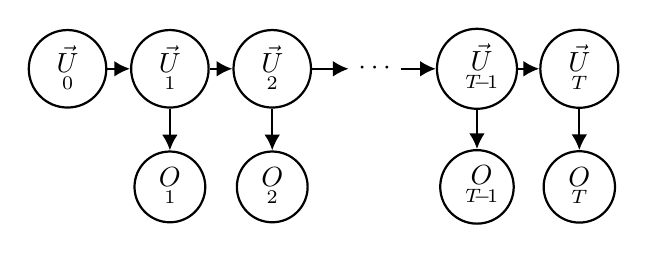
\begin{tikzpicture}[node distance=1.3cm, >={Latex[length=2mm, width=2mm]}, 
            obs/.style={circle, draw, align=center, text width = 3mm, minimum size=3mm, thick, font=\sffamily},
            lat/.style={rectangle, draw, align=center, text width = 6mm, minimum size=6mm, thick, font=\sffamily}]
            
            % Nodes
            \node[obs] (U0) {$\underset{0}{\vec{U}}$};
            \node[obs, right of=U0] (U1) {$\underset{1}{\vec{U}}$};
            \node[obs, right of=U1] (U2) {$\underset{2}{\vec{U}}$};
            \node[right of=U2] (dots) {$\cdots$};
            \node[obs, right of=dots] (UTb) {$\underset{T\!\!-\!1}{\vec{U}}$};
            \node[obs, right of=UTb] (UT) {$\underset{T}{\vec{U}}$};
            
            \node[obs, below of=U1, yshift=-0.2cm] (O1) {$\underset{1}{O}$};
        \node[obs, below of=U2, yshift=-0.2cm] (O2) {$\underset{2}{O}$};
        \node[obs, below of=UTb, yshift=-0.2cm] (OTb) {$\underset{T\!\!-\!1}{O}$};
        \node[obs, below of=UT, yshift=-0.2cm] (OT) {$\underset{T}{O}$};
        
        % Edges
        \draw[->, thick] (U0) -- (U1);
        \draw[->, thick] (U1) -- (U2);
        \draw[->, thick] (U2) -- (dots);
        \draw[->, thick] (dots) -- (UTb);
        \draw[->, thick] (UTb) -- (UT);
        
        \draw[->, thick] (U1) -- (O1);
        \draw[->, thick] (U2) -- (O2);
        \draw[->, thick] (UTb) -- (OTb);
        \draw[->, thick] (UT) -- (OT);    
    \end{tikzpicture}
\end{center}

How did we generate figures \ref{fig:iwps}? We express the factorized joint distribution of the Integrated Wiener Process using Matrix Fraction Decomposition for eqs. \ref{eq:easy_matrix_exponential} and \ref{eq:hard_matrix_exponential}, choose an initial distribution\footnote{The figures use a deterministic initial distribution $\vec{U}(0) \sim \mathcal{N}(\mathbf{0}^n, \mathbf{0}^{n \times n})$}.

The chain-structure of the bayesian network can be exploited to compute the posterior in time $O(|\mathbb{T}|n^3)$(\cite{probnum}) which increases linearly with time. The Kalman-filter and -smoother can be used to compute the full posterior distribution given linear (possibly noisy) transformations $Y_i$ of the state $\vec{U}_i$ at each time.
If one were to form the full joint distribution as one long mean-vector and covariance matrix, the cost of computing the posterior would be of order $O(|\mathbb{T}|^3n^3)$ by the cubic cost of matrix inversion required for the covariance matrix.




\subsection*{Hypothesis: Heat Prior, Wave Prior}
\definition{Heat Prior, Wave Prior}{What is it?}



\ifdefined\COMPILINGFROMMAIN
\else    
    \end{document}
\fi

\clearpage
\section{Applying the Solver}\label{sec:solver_experiments}
\ifdefined\COMPILINGFROMMAIN
\else
    %%%%HEADER
\documentclass[twocolumn]{article}
\usepackage[a4paper, margin=1in, columnsep=20pt]{geometry}
\usepackage{amsmath, amssymb, graphicx, hyperref}
\usepackage[most,skins,breakable]{tcolorbox}
\usepackage[symbol]{footmisc}
\usetikzlibrary{calc}
\usepackage{xcolor}
\usepackage{caption}
\usepackage{algorithm}
\usepackage{algpseudocodex}
\usepackage{tikz}
\usepackage{listings}
\usetikzlibrary{arrows.meta, positioning}
\tcbuselibrary{listingsutf8}
\usepackage{microtype}
\usepackage{blindtext}
\usepackage{bookmark}
\usepackage{breqn}
\usepackage[backend=biber,style=numeric]{biblatex} % 
\addbibresource{../references.bib}

% Define style for the listings environment
\lstdefinestyle{mystyle}{
    basicstyle=\ttfamily\small,
    breaklines=true,
    escapeinside={(*@}{@*)}, % Allows math mode within listings
    numbers=left,
    numberstyle=\tiny,
    frame=single,
    keywordstyle=\color{blue}\bfseries,
    commentstyle=\color{green!50!black},
    stringstyle=\color{red}
}


\def\reals{\mathbb{R}}
% Define the custom definition box and command
\newtcolorbox{mydefinition}[2][]{%
    text width=0.95\columnwidth,
    before=\vspace{1mm}, 
    after=\vspace{1mm}, 
    colback=gray!10, % Background color (light gray)
    colframe=black!70,  % Border color
    coltitle=gray!10,  % Title color
    fonttitle=\bfseries, % Title font style
    sharp corners,   % Box style
    left=2pt,
    breakable,
    right=2pt,
    top=2pt,
    bottom=2pt,
    enhanced jigsaw,
    title=Definition: {#1},         % Title passed as the first argument
    colupper=black,  % Ensure proper content handling
    pad at break*=1pc,
    overlay first and middle={
        \coordinate (A1) at ($(interior.south east) + (-10pt,5pt)$);
        \coordinate (C1) at ($(interior.south east) + (-6pt,7.5pt)$);
        \draw[fill=black!50] (A1) -- +(0,5pt) -- (C1) -- cycle;
    }
    }
    
\newcommand{\definition}[2]{%
    \noindent%
    \begin{mydefinition}[#1]%
        .#2%
    \end{mydefinition}%
    \noindent
}

\newtcolorbox{myexample}[2][]{%
    text width=0.95\columnwidth,
    before=\vspace{1mm}, 
    after=\vspace{1mm}, 
    colback=orange!3, % Background color (light gray)
    colframe=black!70,  % Border color
    coltitle=gray!10,  % Title color
    fonttitle=\bfseries, % Title font style
    sharp corners,   % Box style
    left=2pt,
    right=2pt,
    top=2pt,
    bottom=2pt,
    breakable,
    title=Intuition: {#1},         % Title passed as the first argument
    pad at break*=1pc,
    overlay first and middle={
        \coordinate (A1) at ($(interior.south east) + (-10pt,5pt)$);
        \coordinate (C1) at ($(interior.south east) + (-6pt,7.5pt)$);
        \draw[fill=black!50] (A1) -- +(0,5pt) -- (C1) -- cycle;
    }
}

\newcommand{\example}[2]{%
    \noindent%
    \begin{myexample}[#1]%
    .#2%
    \end{myexample}%
    \noindent
}

\newtcolorbox{algobox}[2][]{%
    text width=0.95\columnwidth,
    before=\vspace{1mm}, 
    after=\vspace{1mm}, 
    colback=blue!5, % Background color (light gray)
    colframe=black!70,  % Border color
    coltitle=gray!10,  % Title color
    fonttitle=\bfseries, % Title font style
    sharp corners,   % Box style
    left=2pt,
    right=2pt,
    top=2pt,
    bottom=2pt,
    breakable,
    title=Algorithm: {#1},         % Title passed as the first argument
    pad at break*=1pc,
    overlay first and middle={
        \coordinate (A1) at ($(interior.south east) + (-10pt,5pt)$);
        \coordinate (C1) at ($(interior.south east) + (-6pt,7.5pt)$);
        \draw[fill=black!50] (A1) -- +(0,5pt) -- (C1) -- cycle;
    }
}

\newcommand{\algorithmbox}[2]{%
\noindent%
    \begin{algobox}[#1]%
    .#2%
    \end{algobox}%
    \noindent
}
%%%%HEADER

    \begin{document}
\fi
\noindent
Here, we give some demonstrations of the Laplacian matrices we have built, solved with built PN solver from chapter \ref{sec:prior}. We will use the colormap in figure \ref{fig:colorbar} for all figures in this section.
\\
\begin{center}
    
\includegraphics[width=1.0\columnwidth]{../images/colorbar.png}
    \captionof{figure}{Colorbar for the figures in this section, using the perceptually uniform \texttt{viridis} \cite{viridis} colormap. The associated scalar values will generally not be exactly given, as they are not important for the interpretation of the figures. However, generally, dark value are negative, light values are positive, and the midpoint is zero.}
    \label{fig:colorbar}
\end{center}
\noindent

\section{Demonstrations}
\subsection*{Solving the Poisson Problem}
Here we demonstrate the Laplacians built one some meshes. These are solutions of the Poisson problem on the 2D surface of various shapes - since they are not time-varying, they will not be solved using our PN solver, but can be solved by a linear solver. The Poisson problem is given by:
\begin{align}
    -\Delta u = f
\end{align}
On a mesh with the discrete Laplacian $L$, this reduces to finding the vector $u$ such that $Lu = f$, which is straightforward to solve with numerical linear algebra tools. For this example, we solve the Poisson problem on a model of a twisty section of kelp. The curvature of the kelp is encoded in the Laplacian matrix. Since this two-dimensional surface has a boundary, we must specify boundary conditions: We set both opposing pairs of edges to the same color, some positive and negative value, respectively (Dirichlet boundary conditions). The solution is illustrated in figure \ref{fig:helix}. The topmost figure shows the boundary conditions (the interior is set to zero for this visualization). The middle figure shows the force $f$, which is a positive Gaussian bell on the interior. The bottommost figure shows the computed solution, which satisfies the hot/cold boundary conditions, while the interior satisfies the curvature dictated by $f$.

\begin{figure}
    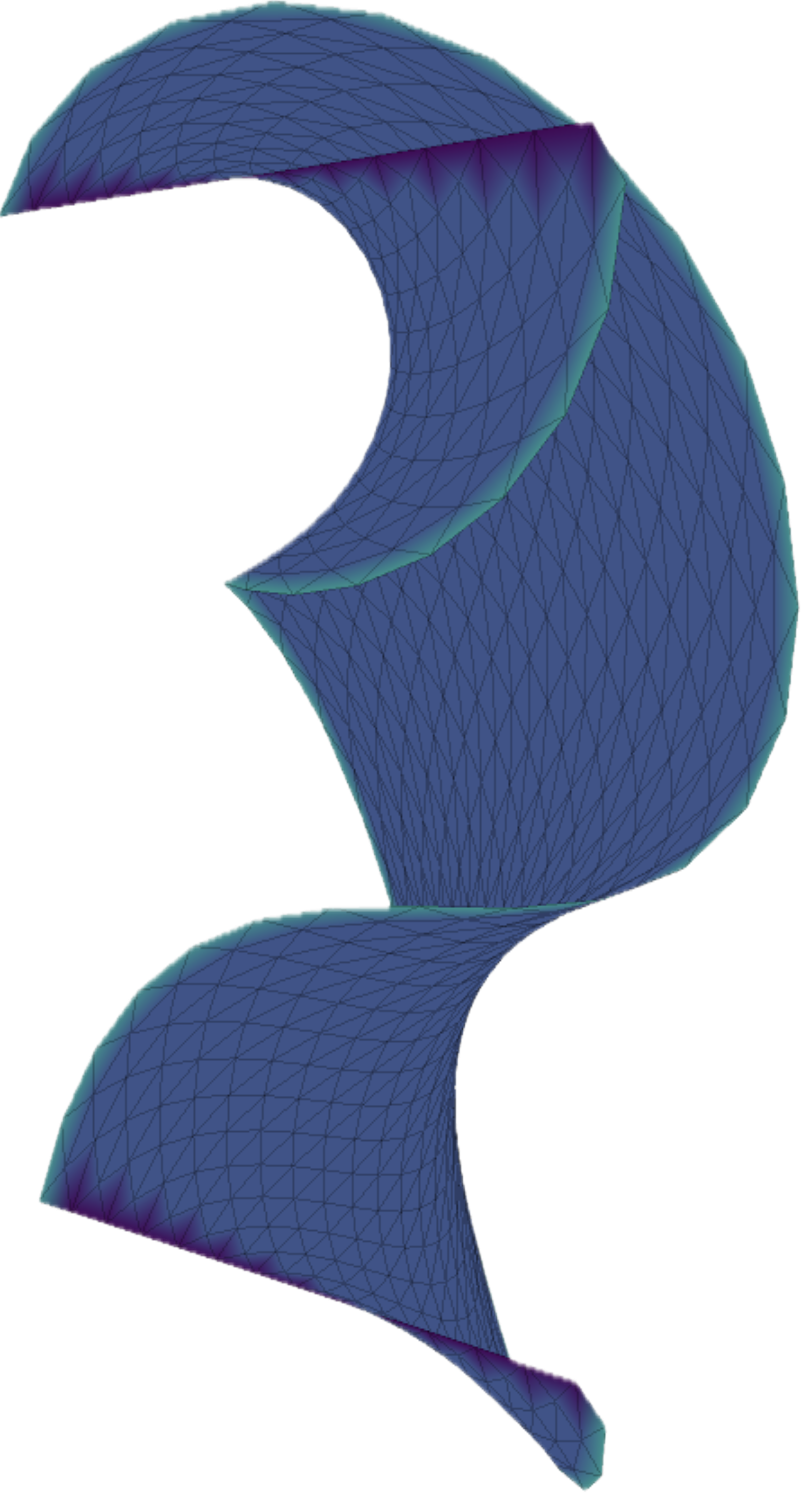
\includegraphics[width=0.95\linewidth]{../images/helix_BC.png}
    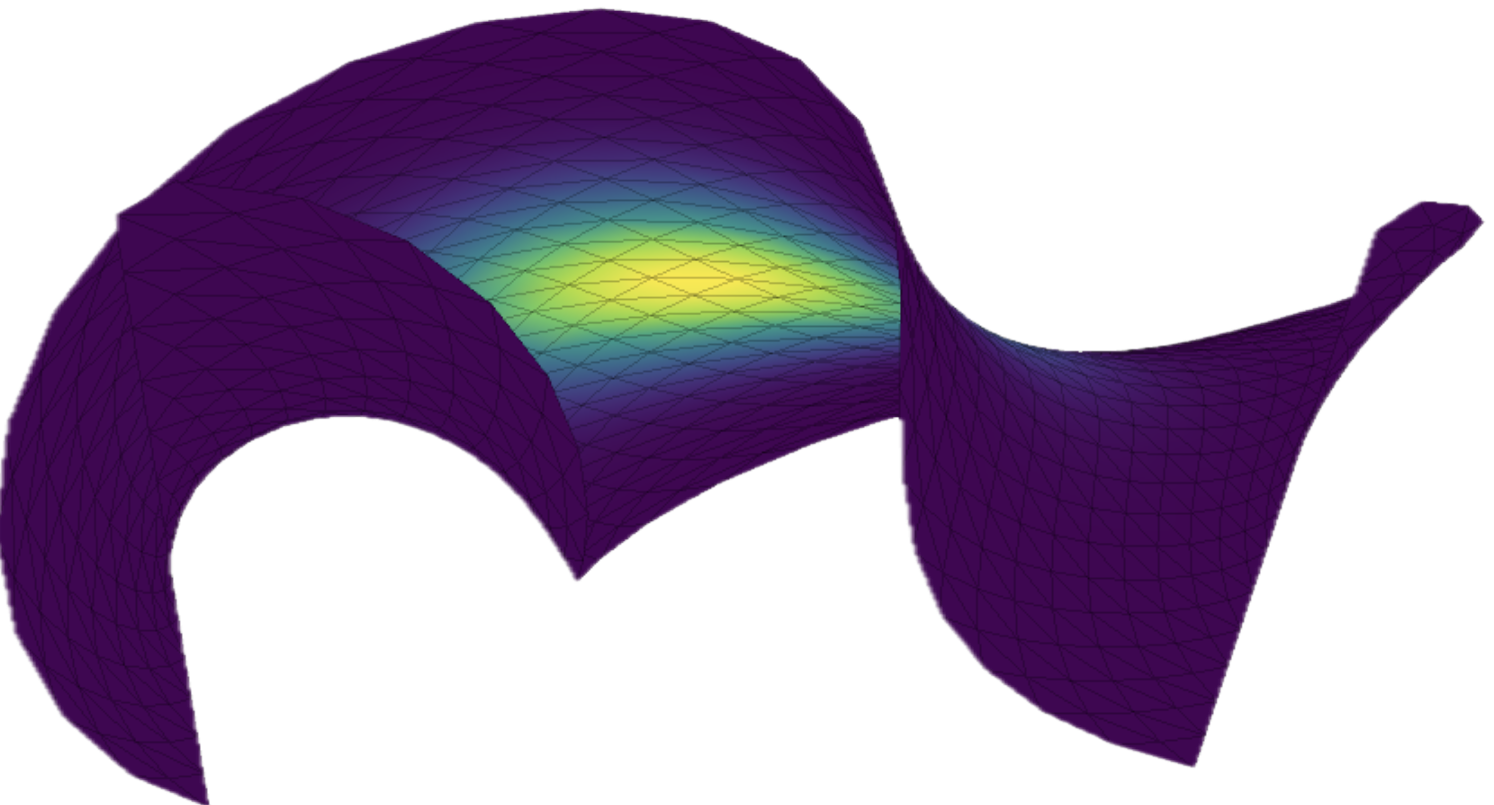
\includegraphics[width=0.95\linewidth]{../images/helix_force.png}    
    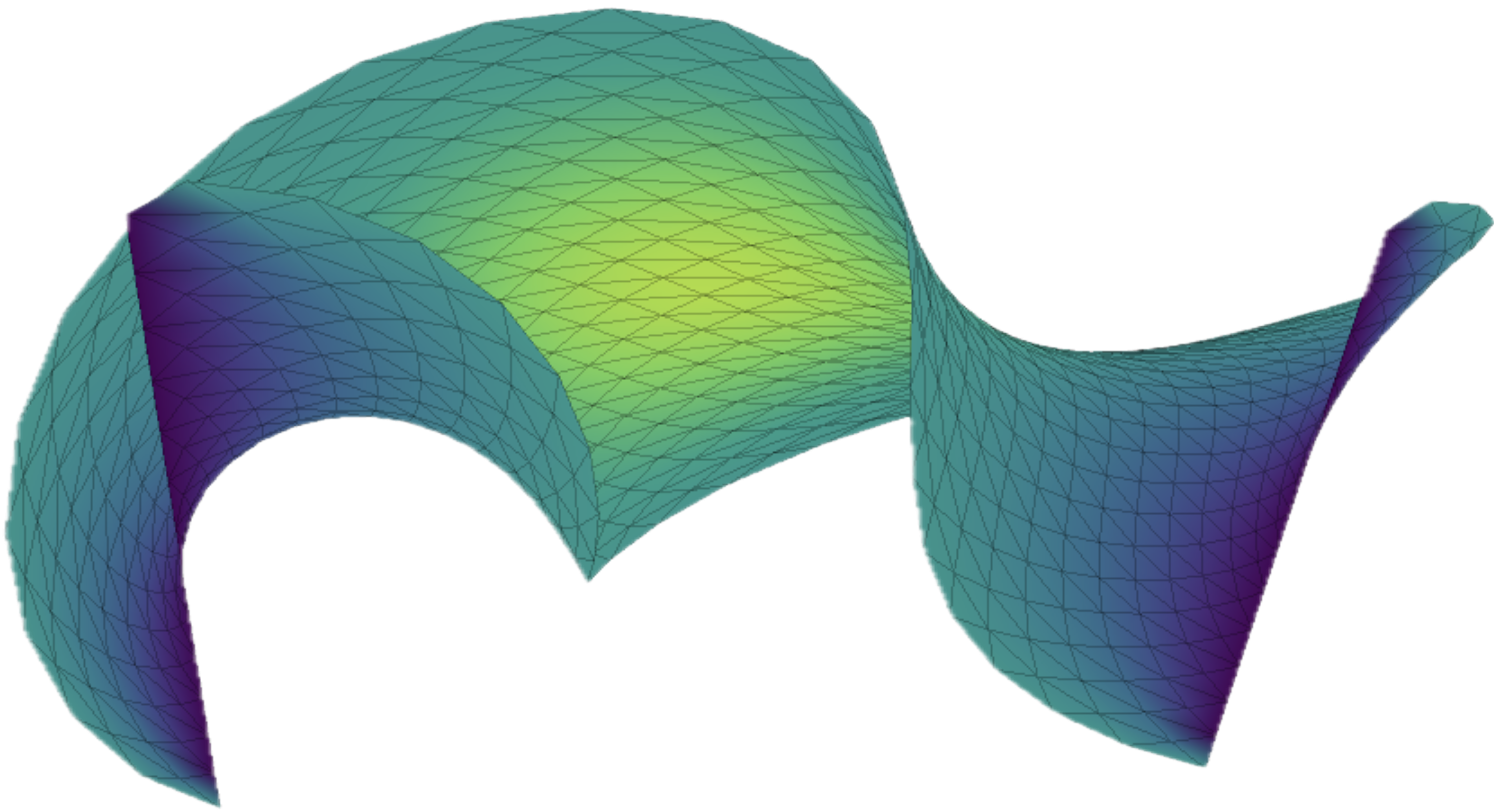
\includegraphics[width=0.95\linewidth]{../images/helix_solution.png}
    \captionof{figure}{}
    \label{fig:helix}
\end{figure}


\subsection*{Solving the Heat Equation}
As a demonstration, using the probabilistic solver, we solve the heat equation on the sphere, using the twice-integrated Wiener process. The speed of diffusion is linked to the Laplacians matrix $L$, which in turn depends on the scale of the geometry. We will therefore not give any units or specific values which are unimportant. See figure \ref{fig:heat_solution} for a demonsration of the solver. In figure can additionally get the joint distribution of the solution and show the uncertainties, see figure \ref{fig:heat_uncertainty}. We interpret the nonuniformity of the figure in the following way: The sphere mesh used has twelve\footnote{This mesh is created by using loop subdivision on the 12-tipped icosahedron with the \texttt{icosphere} Python package, which is a coarse approximation to the sphere geometry.} patches of vertices with incidence number 5 - in these, the solution is more certain than in the remaining ones. The Laplacian matrix will have five nonzero entries in the corresponding rows instead of six, and thus the solution here is less sensitive to the values of the neighbors. Additionally, the neighboring five vertices are spatially closer (the edge lengths are shorter), which introduces higher correlation between them.

\begin{center}
    \begin{minipage}[b]{0.5\columnwidth}
        \centering
        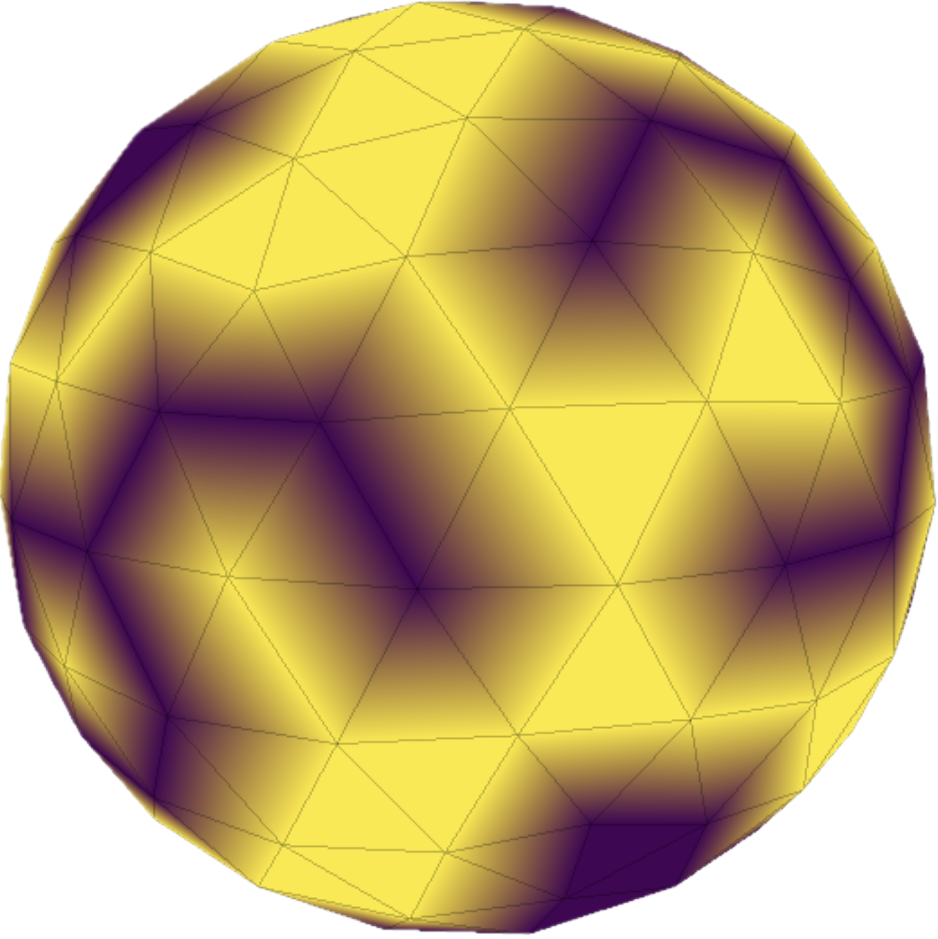
\includegraphics[width=0.95\linewidth]{../images/sphere_entropic.png}
    \end{minipage}%
    % \hspace{5mm} 
    \begin{minipage}[b]{0.5\columnwidth}
        \centering
        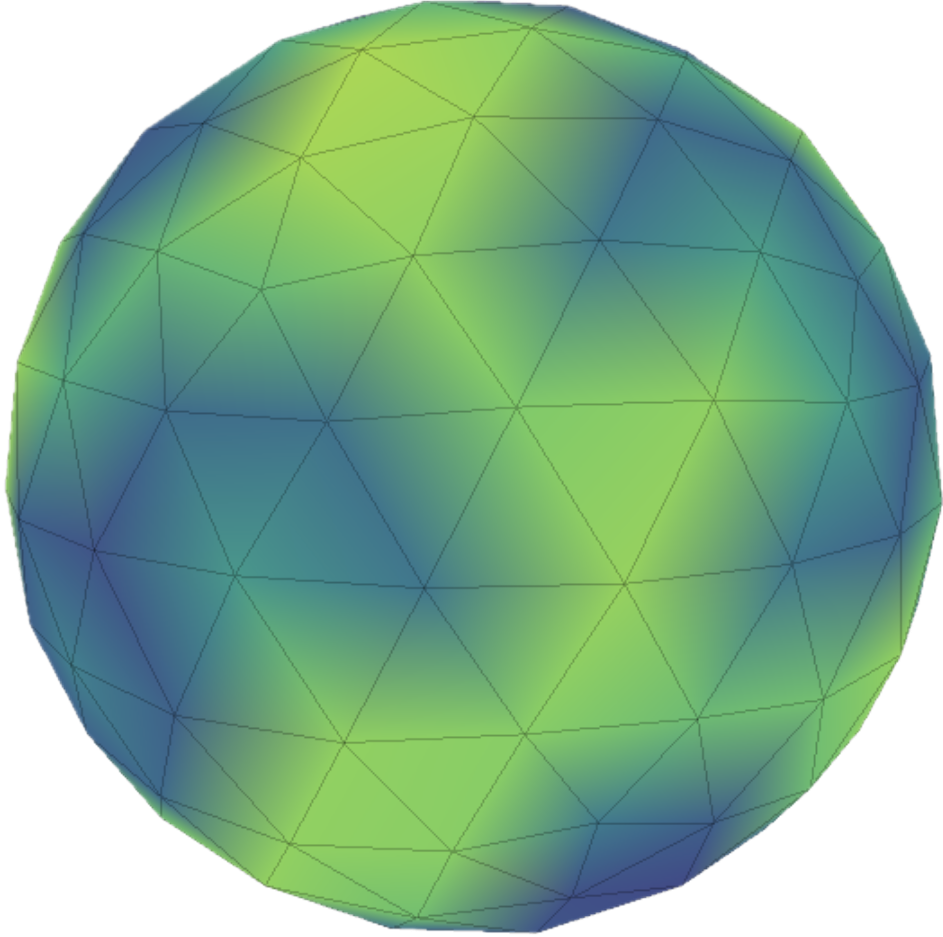
\includegraphics[width=0.95\linewidth]{../images/sphere_smoothed.png}
    \end{minipage}
    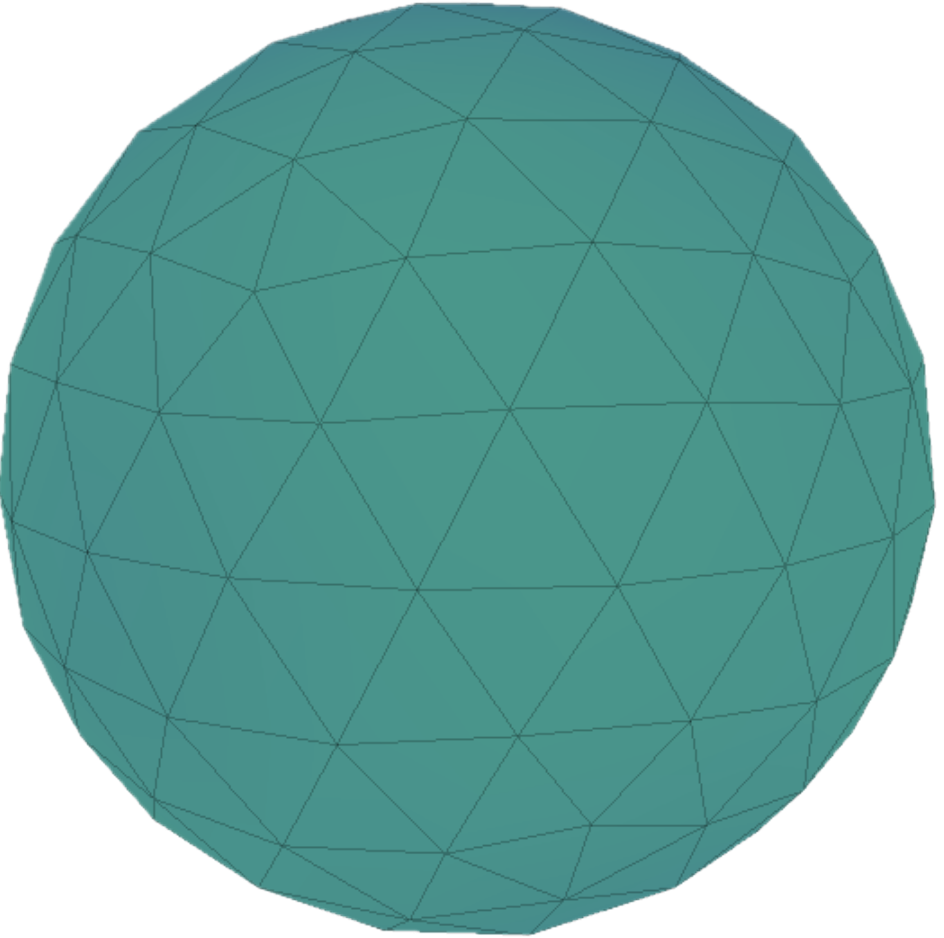
\includegraphics[width=0.475\columnwidth]{../images/sphere_cooled.png}\vspace*{3mm}
    \captionof{figure}{The heat equation solved on the sphere. Upper left image is the initial temperature distribution, where each vertex has been assigned to $\{-1, 1\}$ uniformly at random. Upper right and lower image are spaced equally apart in time, illustrating the heat diffusion. Yellows are positive temperatures, blues are negative temperatures.}
    \label{fig:heat_solution}
\end{center}

\begin{center}
    \vspace{10mm}
    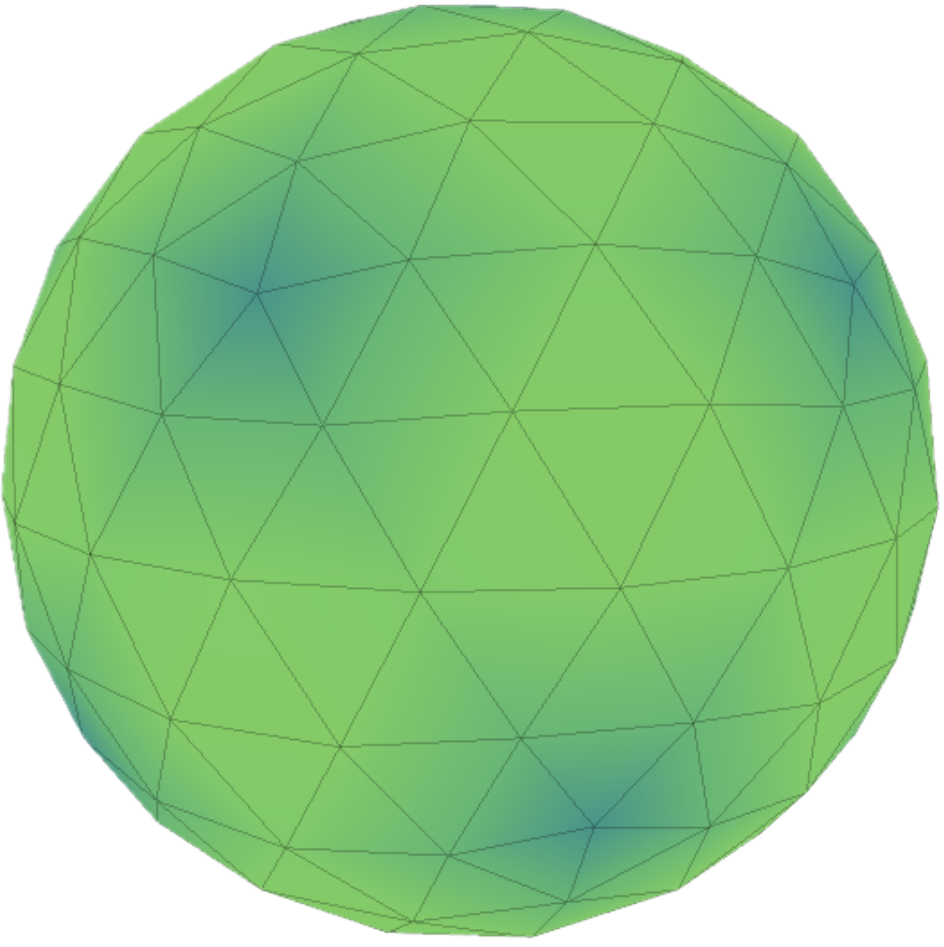
\includegraphics[width=0.7\columnwidth]{../images/sphere_uncertainty.png}\vspace*{3mm}
    \captionof{figure}{The marginal standard deviations of the solution at the second step in figure \ref{fig:heat_solution}. Darker colors mean lower uncertainty. The uncertainty is miniscule and has been scaled up for illustration.}
    \label{fig:heat_uncertainty}
\end{center}

\example{The Laplacian captures the length-scale}{   
    We visualize the Laplacian capturing length-scales on the Utah teapot \cite{utah} has been scaled so the body of the teapot is approximately a unit sphere. Figure \ref{fig:teapot_heat_solution} shows again the heat equation initial step and a short time later. The Utah teapot has highly non-uniform dual face areas, especially around the rim at the lid. As the diffusion process is not scale-invariant is illustrated by the fact that the temperature here will smooth out much quicker than in the remaining, bigger patches.
    \begin{center}
        \centering
        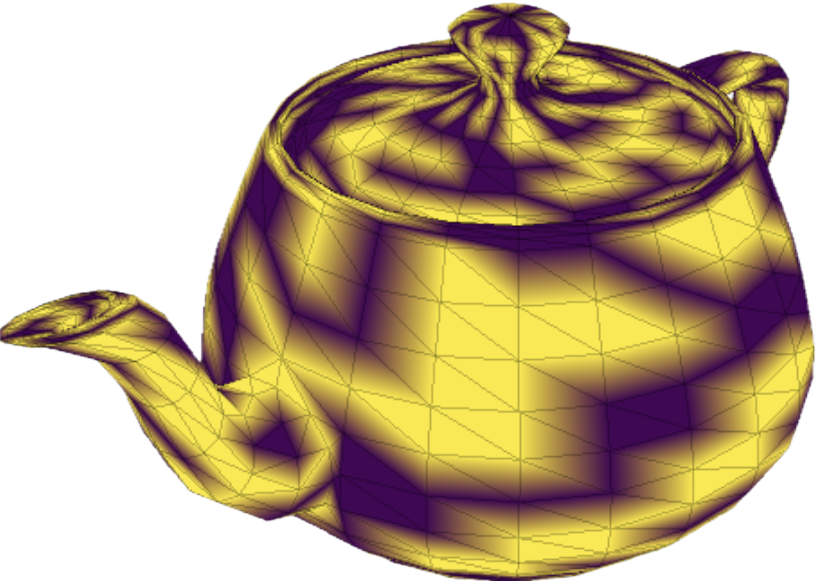
\includegraphics[width=0.9\columnwidth]{../images/teapot_entropic.png}\vspace*{3mm}
        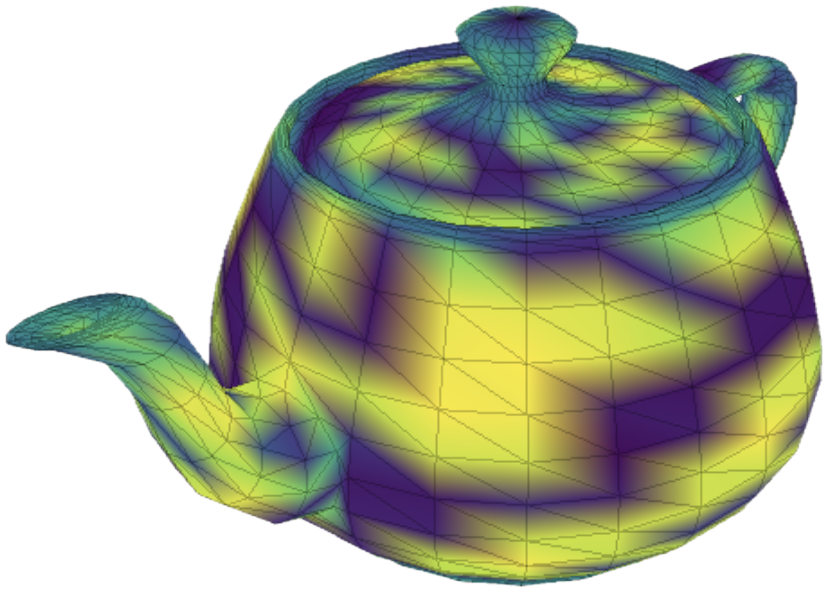
\includegraphics[width=0.9\columnwidth]{../images/teapot_smoothed.png}\vspace*{3mm}
        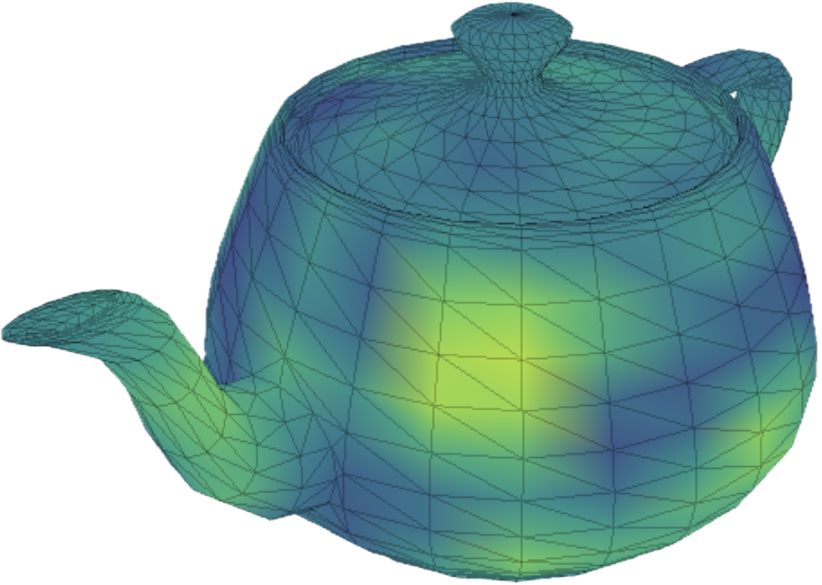
\includegraphics[width=0.9\columnwidth]{../images/teapot_cooled.png}\vspace*{3mm}
        \captionof{figure}{The heat equation being solved on the Utah Teapot. Top: The initial conditions are akin to the ones in fig. \ref{fig:heat_solution} and shown in the topmost figure. Middle: Heat diffusion after a short time. Bottom: Heat diffusion after a longer time.}
        \label{fig:teapot_heat_solution}
    \end{center}
}

\subsection*{Solving the Wave Equation On an Intrinsically Triangulated Surface}
Using our algorithm from chapter \ref{sec:intrinsic_triangulation}, we use triangulate the bell-curve geometry, compute the Laplacian, and solve the wave equation on it. To motivate the expected behaviour, one can think of a wave as simply a shockwave traveling at constant speed from a source, which we visualize an approximation of in figure \ref{fig:dijkstra}. There are multiple ways to compute the location of the front of the shockwave, such as the ones proposed and compared in \cite{vector_dijkstra} and \cite{heat_method}. For the sake of ease of implementation, we use the simplest one, Dijkstra's single-source-all-paths algorithm. The figure shows level-sets of the distance function to the source (on the left, at coordinates $(-0.5, 0.0)$). This figure suggests that one should observe the wave traveling around the bump faster than across it, which is reasonable, given the detour the wave would take to travel across the bump.
This simplification ignores the reflections and interference that might occur due to our Dirichelet BCs (which are fixed at a wave-height of zero).
\\
The four stacked planes in figure \ref{fig:bell_wave}, show the solution of the wave equation on the intrinsic bell-curve mesh.
\label{fig:bell_wave}
\newpage
\begin{center}
    \centering
    \hspace*{-6mm}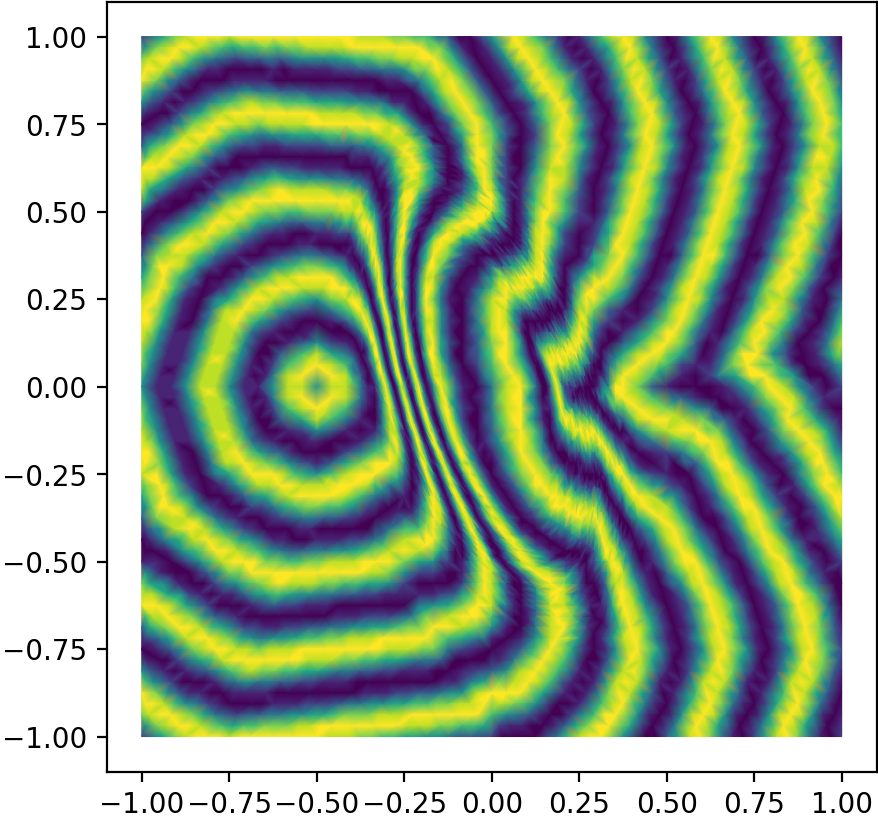
\includegraphics[width=0.9\columnwidth]{../images/bell_wave_distances.png}
    \captionof{figure}{Level sets of the distance function from a source at coordinates $(-0.5, 0.0)$ on the intrinsic triangulation of the Gaussian bump mesh. The wave equation is solved on this mesh in the following figure.}
    \label{fig:dijkstra}
    \vspace*{10mm}
    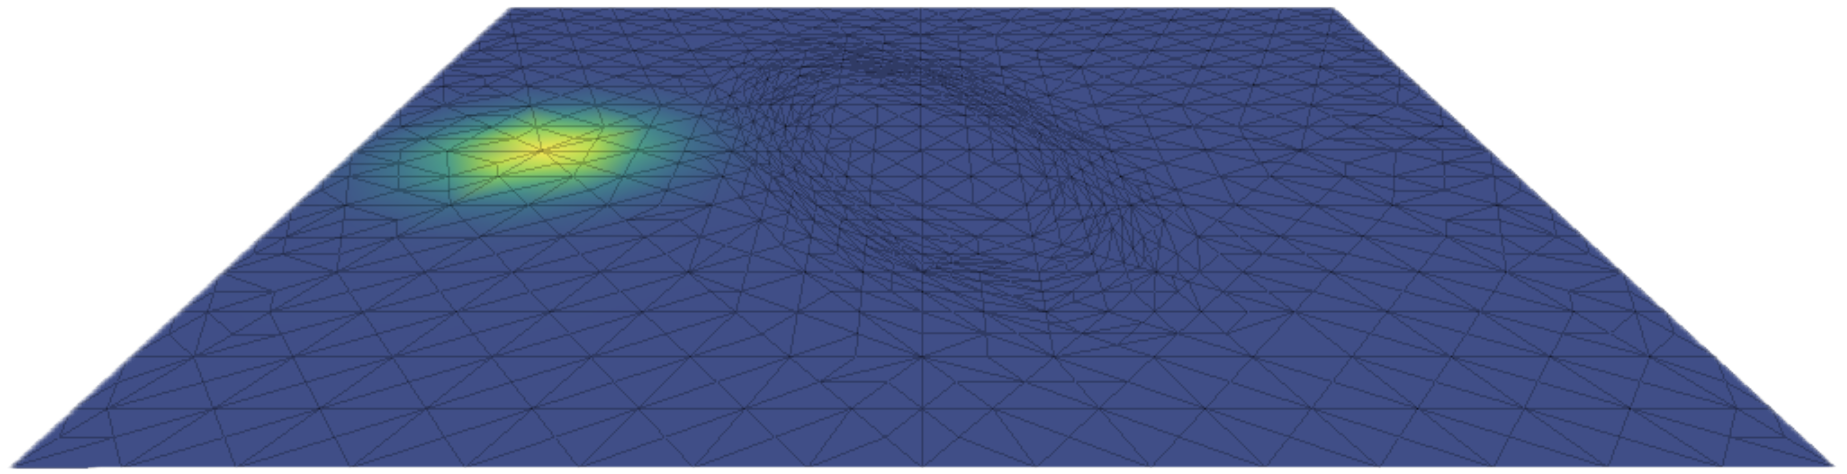
\includegraphics[width=\columnwidth]{../images/bell_wave_0.png}\vspace*{3mm}
    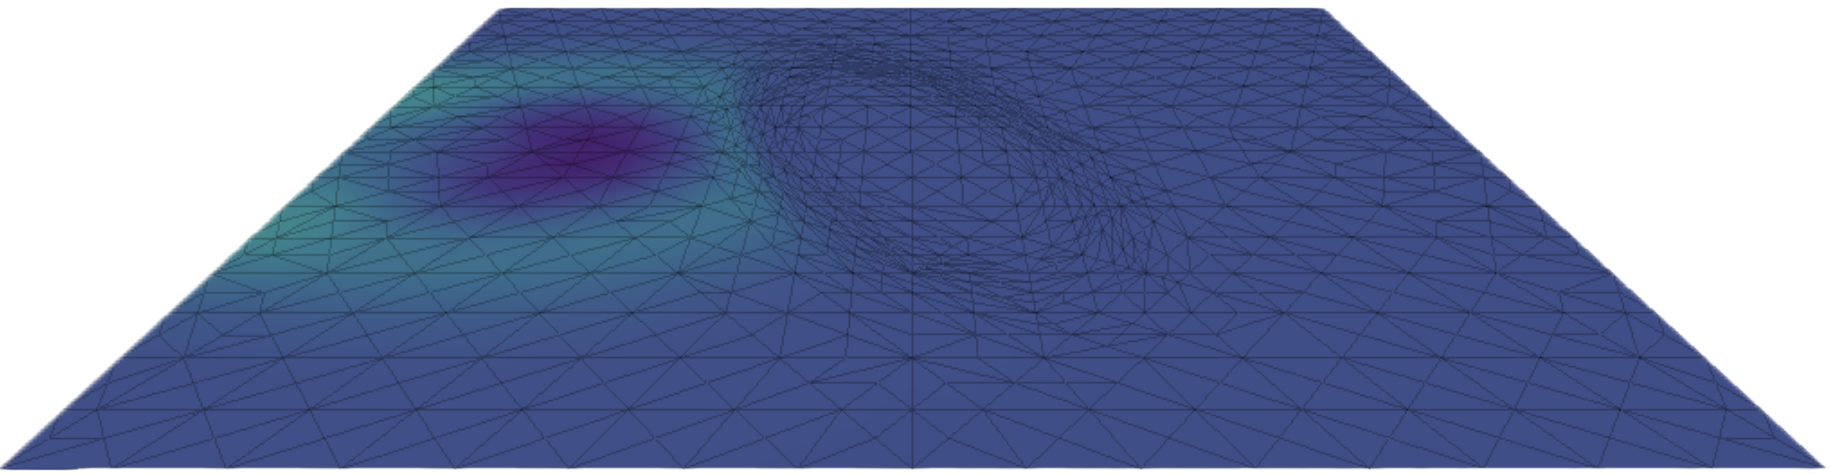
\includegraphics[width=\columnwidth]{../images/bell_wave_1.png}\vspace*{3mm}
    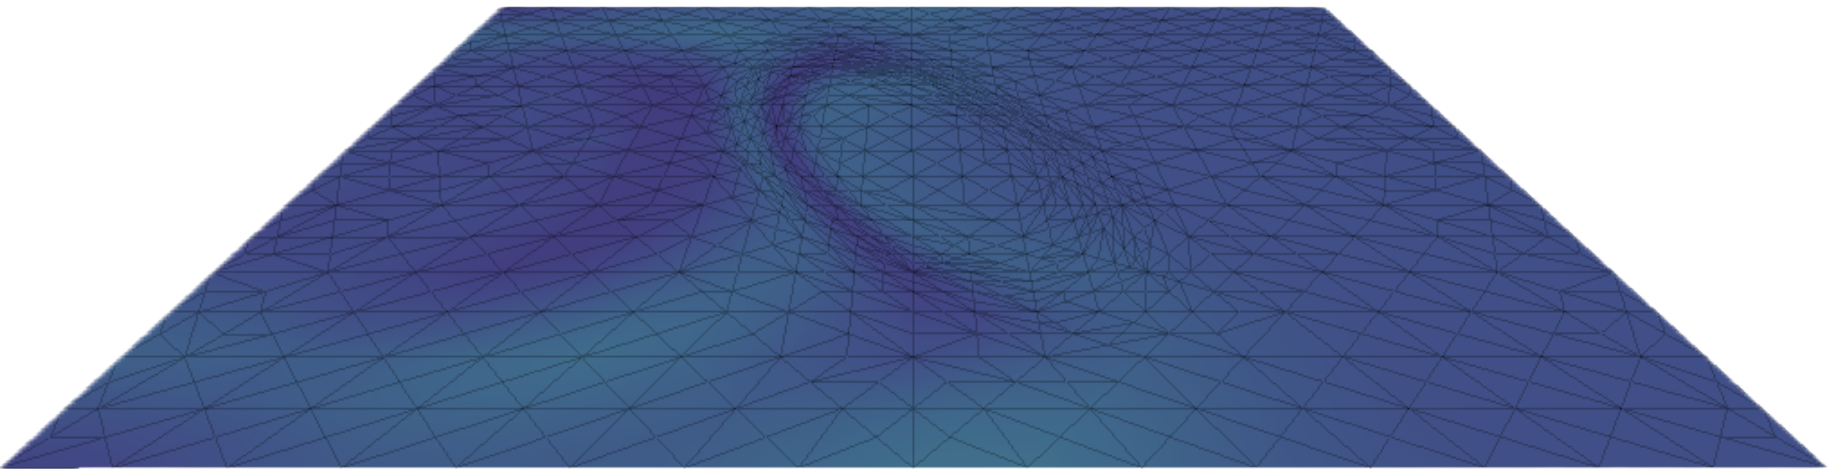
\includegraphics[width=\columnwidth]{../images/bell_wave_2.png}\vspace*{3mm}
    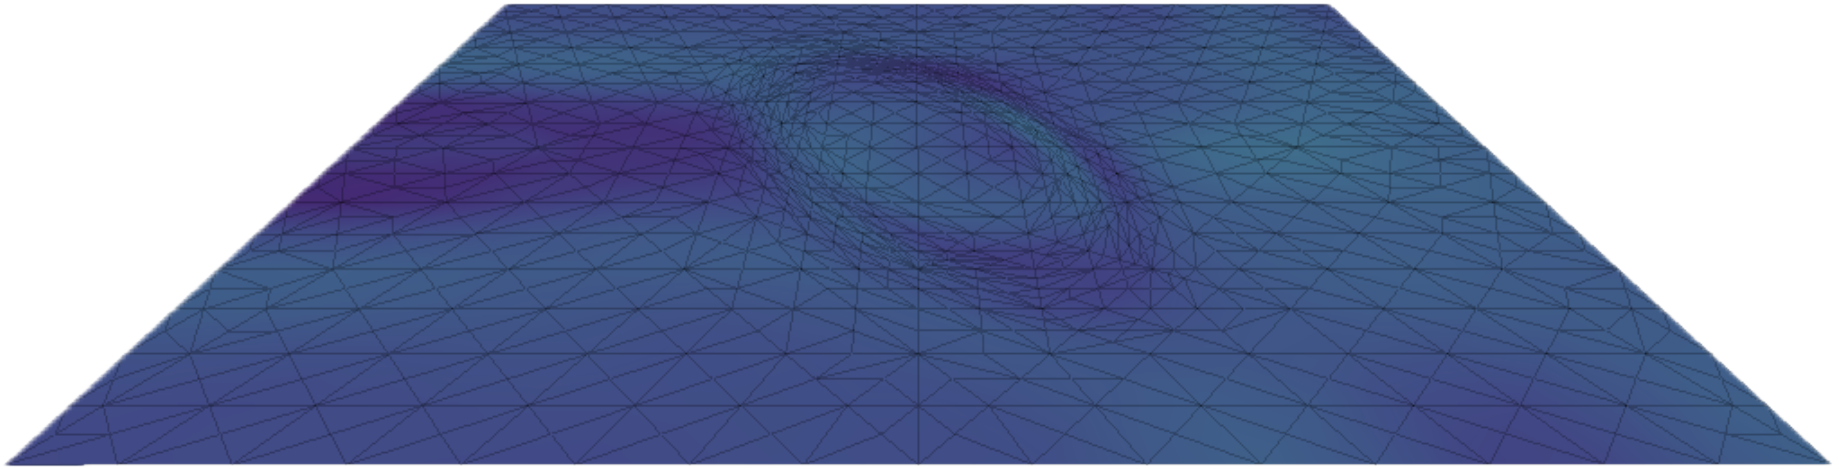
\includegraphics[width=\columnwidth]{../images/bell_wave_3.png}\vspace*{3mm}
    \captionof{figure}{From top to bottom, four consecutive equally spaced instants of the wave equation on the intrinsic triangulation of the Gaussian bump mesh. The initial condition is given in the topmost picture. In the third picture from the top, there are clear similarities with the shapes shown in \ref{fig:dijkstra} when comparing the shape of the wave around the bump. We emphasize that the mesh is completely intrinsic and "flat" - there is no extrusion of the bump on this mesh.}
    \label{fig:bell_wave}
\end{center}

\section{Experiments with Physically Informed Priors}
As problems to study, we choose a nonlinear version of the heat (\ref{eq:nonlinear_heat}) and wave (\ref{eq:nonlinear_wave}) equation, with varying degrees of nonlinearity. 
\begin{align}
    \frac{\partial}{\partial t}u = -\Delta u - \alpha u^2\label{eq:nonlinear_heat}
\end{align}
\begin{align}
    \frac{\partial^2}{\partial t^2}u = -\Delta u - \alpha\tan u\label{eq:nonlinear_wave}
\end{align}
The hypothesis is that, for small nonlinearities, a prior that encodes the linear heat/wave dynamics will outperform the integrated Wiener process. 

\subsection*{Encoding the Linear part of a PDE into a Prior}
This idea is adapted from \cite{exponential_probabilistic} in which the authors show that using integrated Ornstein-Uhlenbeck processes (chapter \ref{sec:prior}) give an inductive bias when solving ODEs with partially linear dynamics (semilinear ODEs / PDEs). Using such a prior leads to faster convergence than the usual integrated Wiener process, because it exactly solves the linear part of the ODE.
We show that the same idea can be applied to PDEs and give appropriate prior process, but will start by explaining the principle.
\\
\example{Mean of Prior solves Linear ODE exactly}{
We can take any linear ODE and make a series of transformations to the ODE that preserve the modeled system, but will explicitly model more derivatives in the state space.
\\
We will show the procedure with the damped harmonic oscillator
\begin{align}
    \frac{d}{dt}\vec{u}_0 &= \vec{u}_1 \label{eq:physics_prior_0}
    \\\frac{d}{dt}\vec{u}_1 &= -a\vec{u}_{0} - b\vec{u}_{1}\label{eq:physics_prior_1}
\end{align}
for some fixed choice of $a$, $b$.
\\
Assume we are given initial condition $\vec{u}_0(0)=s_0(0)$, $\vec{u}_1(0) = s_1$. We can feed the initial known values into eq. \ref{eq:physics_prior_1} to get $s_2 = \vec{u}_2(0) = -a\vec{u}_{0}(0) - b\vec{u}_{1}(0)$.
We now impose regularity on $\vec{u}_2$ by taking the derivative w.r.t. time on all terms in the equations \ref{eq:physics_prior_0} and \ref{eq:physics_prior_1}:
\begin{align*}
    \frac{d^2}{dt^2}\vec{u}_0 &=  \frac{d}{dt}\vec{u}_1 \nonumber
    \\
    \frac{d^2}{dt^2}\vec{u}_1 &=  \frac{d}{dt} \left(-a\vec{u}_{0} - b\vec{u}_{1}\right)
    \\
    &=  -k\frac{d}{dt}\vec{u}_{0} - l\frac{d}{dt}\vec{u}_{1}
\end{align*}
By the derivative/integral relationship in the state-space representation, this simplifies to
\begin{align}
    \frac{d}{dt}\vec{u}_0 = \vec{u}_1
    \\
    \frac{d}{dt}\vec{u}_1 &= \vec{u}_2 \nonumber
    \\
    \frac{d}{dt}\vec{u}_2 &= -a\vec{u}_{1} - b\vec{u}_{2}
\end{align}
We have increased the state-space to encompass another derivative. Since we previously determined $\vec{u}_2(0) = s_2$, we have all the required information to solve this ODE.
\\ The steps in this transformation can be repeated indefinitely; one needs to compute the induced initial value of the derivative from the set of equations and then augment the state-space.
We start off with system matrix $F^\prime$, and after $q-1$ repetitions we end up with a system matrix $F\in\reals^{q+1\times q+1}$ 
$$F^\prime\!\! =\! \begin{bmatrix}
0 & 1 \\  \!-a & \!-b
\end{bmatrix} \to F =\! \begin{bmatrix}
0 & 1 & 0 & \!\!\dots\!\! & 0 & 0 & 0 \\
0 & 0 & 1 & \!\!\dots\!\! & 0 & 0 & 0 \\
0 & 0 & 0 & \!\!\dots\!\! & 0 & 0 & 0 \\
\vdots & \!\!\ddots\!\! & \!\!\ddots\!\! & \!\!\ddots\!\! & \!\!\ddots\!\! & \!\!\ddots\!\! & \vdots \\
0 & 0 & 0 & \!\!\dots\!\! & 0 & 1 & 0 \\
0 & 0 & 0 & \!\!\dots\!\! & 0 & 0 & 1 \\
0 & 0 & 0 & \!\!\dots\!\! & 0 & \!\!-a & \!\!\!\!-b \\
\end{bmatrix}$$
The original system matrix $F'$ is nested inside $F$. \\
We conclude by transforming this into a LTI SDE by adding zero mean Brownian motion increments into the highest derivative. When integrated, it will still have zero mean and therefore will not affect the mean of the process. This is similar in spirit to the spring example in chapter \ref{sec:prior}, and yields the following LTI SDE which can directly be applied as a prior.
\begin{align*}
    \frac{d}{dt}\vec{U}_i &= \vec{U}_{i+1} \hspace{10mm} i \in \{0, \dots, q\!-\!1\}
    \\d\;\vec{U}_q &= -b\vec{U}_{q-2}dt - a\vec{U}_{q-1}dt + \sigma dW(t)
\end{align*}
}
\noindent
The previous example was for scalar-valued ODEs, but the same principle can be applied to the state-space representation of vector-valued ODEs like the ones given at the end of chapter \ref{sec:prior}, which can be obtained after applying the Method of Lines to a PDE. The same principle is then simply applied component-wise. For a dimension $n$ vector-valued linear ODE $$\frac{d^2}{dt^2}u = Au + B\frac{d}{dt}u$$ with state-space system matrix $F^\prime$, the corresponding q-times integrated prior will be constructed as
$$F^\prime\!\! =\! \begin{bmatrix}
    \mathbf{0} & \textbf{I}_n \\ \!A & \!B
    \end{bmatrix} \to F = \begin{bmatrix}
\mathbf{0} & \textbf{I}_n & \mathbf{0} & \!\!\!\dots\!\! & \mathbf{0} & \mathbf{0} & \!\!\mathbf{0} \\
\mathbf{0} & \mathbf{0} & \textbf{I}_n & \!\!\!\dots\!\! & \mathbf{0} & \mathbf{0} & \!\!\mathbf{0} \\
\mathbf{0} & \mathbf{0} & \mathbf{0} & \!\!\!\dots\!\! & \mathbf{0} & \mathbf{0} & \!\!\mathbf{0} \\
\vdots & \!\!\ddots\!\! & \!\!\ddots\!\! & \!\!\ddots\!\! & \!\!\ddots\!\! & \!\!\ddots\!\! & \!\!\vdots \\
\mathbf{0} & \mathbf{0} & \mathbf{0} & \!\!\!\dots\!\! & \mathbf{0} & \textbf{I}_n & \!\!\mathbf{0} \\
\mathbf{0} & \mathbf{0} & \mathbf{0} & \!\!\!\dots\!\! & \mathbf{0} & \mathbf{0} & \textbf{I}_n \\
\mathbf{0} & \mathbf{0} & \mathbf{0} & \!\!\!\dots\!\! & \mathbf{0} & \!\!A & \!\!\!\!B \\
\end{bmatrix}$$
We then build the LTI SDE with the diffusion matrix $LL^\top = E_qE_q^\top$, which ensures that the noise is only fed into the highest derivative. \\
This process of repeated integration yields a LTI SDE with $q$ continuous derivatives whose mean coincides with the solution of the original ODE. We now show this for the scalar wave equation and then give the PDE-wave equation counterpart if it is not yet clear how to do this.

\definition{Wave Process Prior}{
    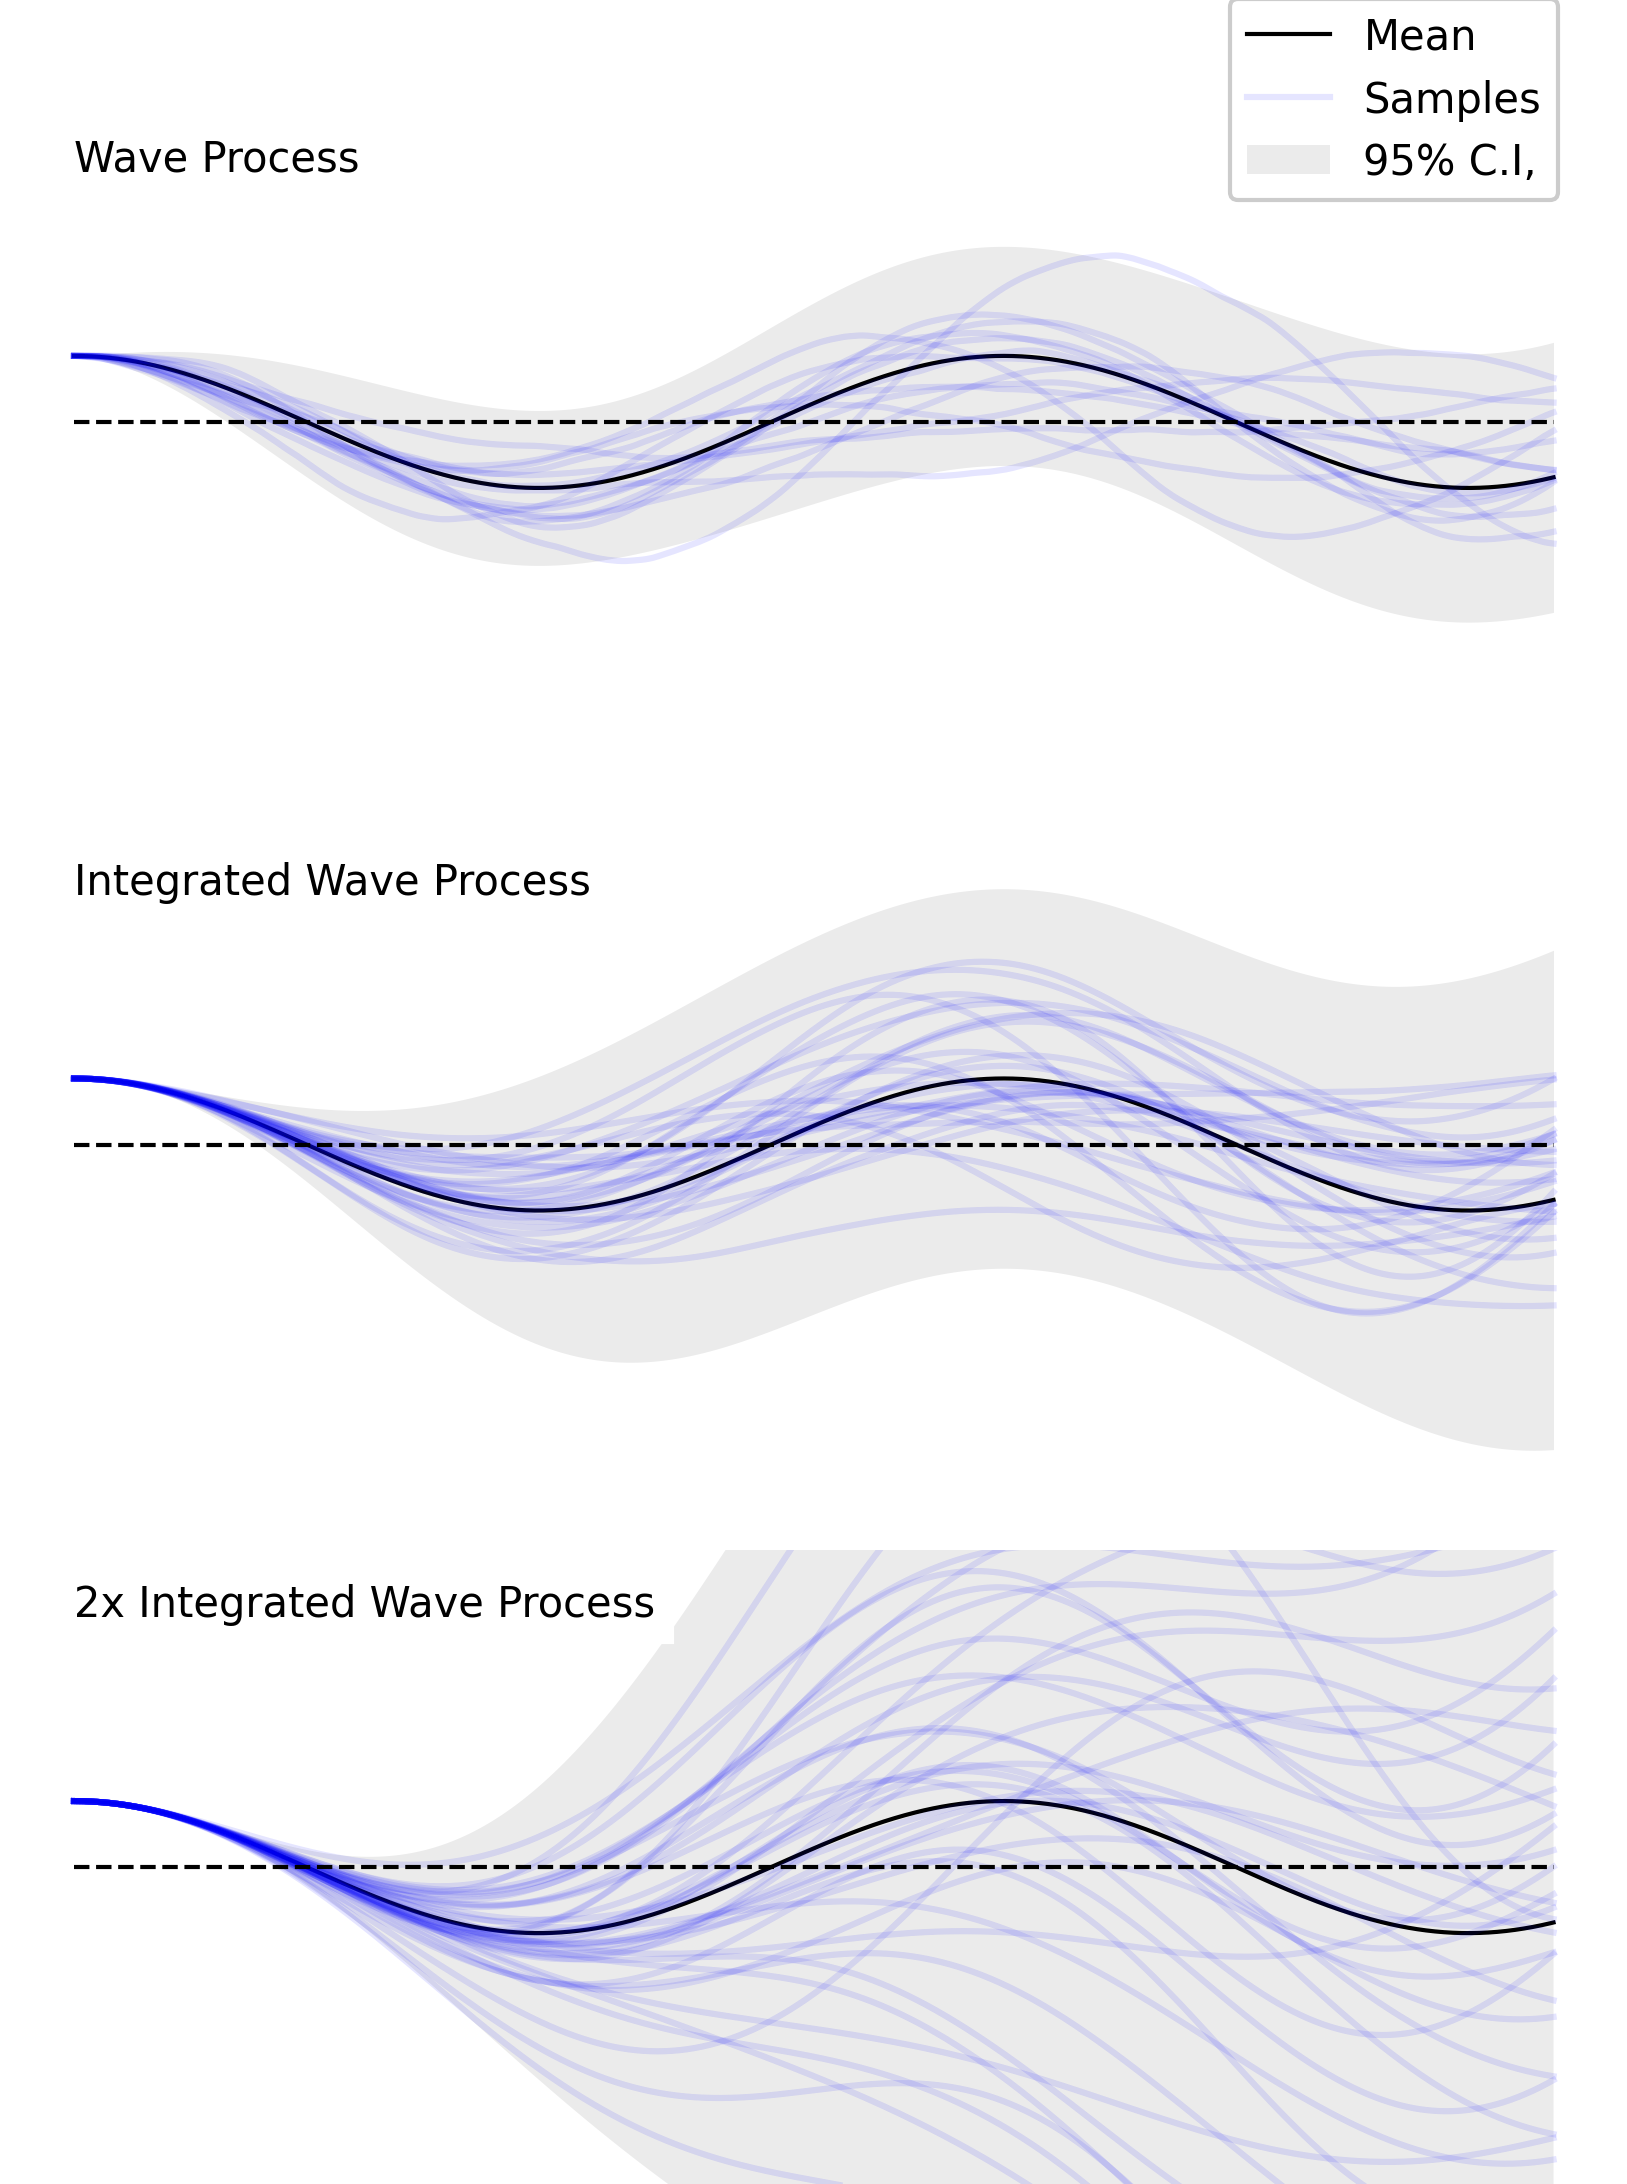
\includegraphics[width=\columnwidth]{../images/wave_process.png}
    \captionof{figure}{Iterated integrations of the Wave Process.}
    \label{fig:wave_process}
    The mean of the scalar wave process solves the scalar wave equation $\frac{d^2}{dt^2}u = -au$ exactly. The simplest scalar wave process has system matrix $F$
    $$F = \begin{bmatrix} 0 & 1 \\ -a & \!0 \end{bmatrix} \hspace*{10mm} L = \begin{bmatrix} 0 \\ 1 \end{bmatrix}$$ 
    (shown at the top), while the once-integrated (middle) wave process has system matrix $F$
    $$F = \begin{bmatrix} 0 & 1 & 0 \\ 0 & 0 & 1 \\ 0 & -a & \!0 \end{bmatrix} \hspace*{10mm} L = \begin{bmatrix} 0 \\ 0 \\ 1 \end{bmatrix}$$
    We initialize the process with the initial conditions calculated from the ODE ($s_0, s_1, \dots$), and the mean will then satisfy the ODE exactly (see figure, exact solution for $a=1$ is $\cos(t)$).
    \\
    \\
    The corresponding process for the wave equation $\frac{d^2}{dt^2}u = -\Delta u$ can be built by discretizing the Laplacian matrix $L$ and using the wave process as the prior, 
    $$F = \begin{bmatrix}
    \mathbf{0} &  \textbf{I}_n  \\ \!-L & \! \mathbf{0}
    \end{bmatrix} \hspace*{5mm} LL^\top = E_1E_1^\top = \begin{bmatrix}
    \mathbf{0} & \mathbf{0} \\ \mathbf{0} & \textbf{I}_n \end{bmatrix}$$
    We will denote this SDE as the Wave Process.
}
\example{Wave Process in Action}{
\begin{center}
    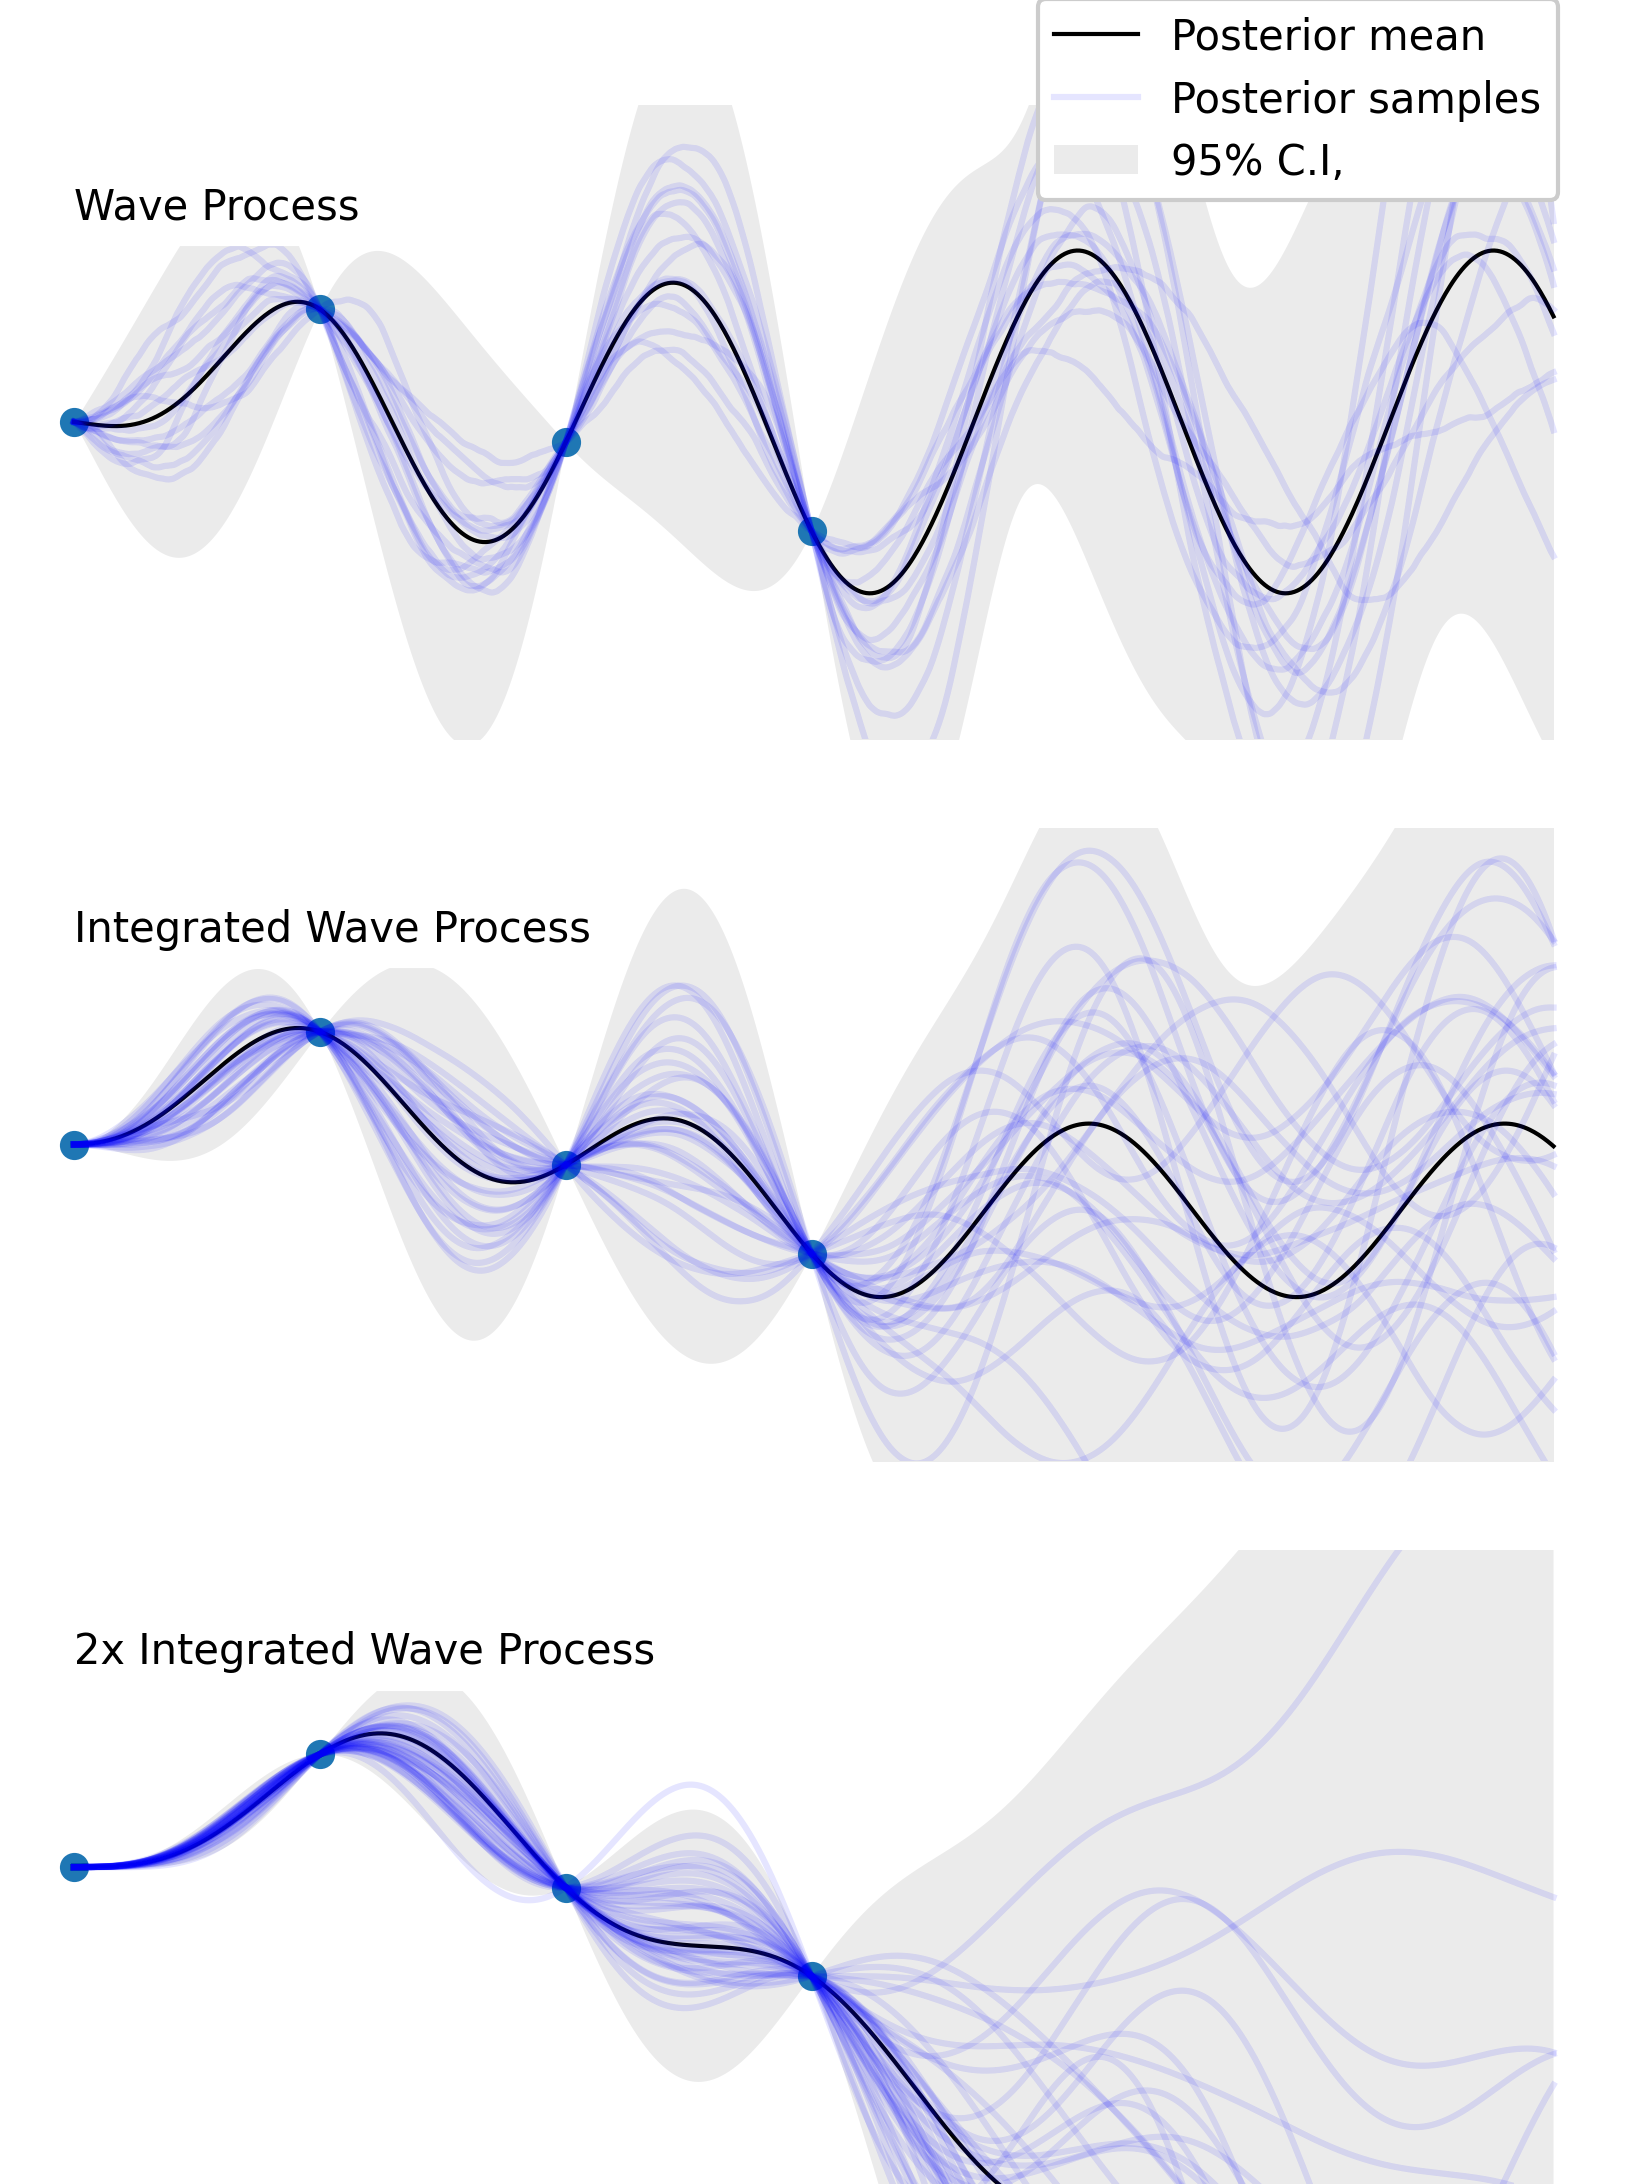
\includegraphics[width=\columnwidth]{../images/conditioned_waves.png}
    \captionof{figure}{Draws from the Integrated Wave Process, Conditioned on the same four points that were also used in chapter \ref{sec:prior}.}
\end{center}
}
\noindent
One is tempted to define a Heat process analogously by placing the Laplacian in the bottom right corner of the dynamics matrix $F$ (which is the correct way of doing it), but it turns out that this reduces to an instance of the Ornstein-Uhlenbeck process with a specific setting of the rate-parameter. We will still refer to it as the Heat process / prior, which captures the spatial diffusion encoded in $L$.

\subsection*{Experiments}
We empirically investigate the efficiency of the probabilistic solver when using the integrated Wiener process, the integrated wave process, and the integrated heat process as priors for the nonlinear heat and wave equations (eq. \ref{eq:nonlinear_heat} \& \ref{eq:nonlinear_wave}).
As the nonlinearities become larger and we move away from the linear dynamics, the prior will not as related and we should expect a decrease in efficiency.  We run both problems for $\alpha\in\{0, 10^{-3}, 1\}$.
\\ For eq. \ref{eq:nonlinear_wave}, we will use integrated Wave processes as our prior, and for eq. \ref{eq:nonlinear_wave} we will use the Heat process. We will compare against repeatedly integrated Wiener processes as priors.
\\\\
The problems will be solved on the 2D surface of the sphere, approximated by a 12-vertex icosphere. The vector fields are integrated from $t_0=0$ to $t_{\mathbb{T}}=10$.  We will grade the PN solutions by the root-mean-square-error at all computed timesteps against a high-accuracy reference solution implemented in \texttt{diffrax} \cite{diffrax}, using the Kvaerno5/4 method \cite{kvaerno}, suitable for stiff problems like the heat and wave equation. The reference solution has both relative and absolute tolerances of $10^{-8}$, which then also serves as a lower bound for the error of the PN solution.
\\ The PN solution will be computed for varying amount of timesteps and for different choices of $q$ in the prior process. We will then plot the work/precision diagrams for the different choices of $q$ and $a$.
\subsection*{Results}
See figures \ref{fig:heat} through \ref{fig:wave big} for all work/precision diagrams. In the figures, the integrated wiener process is depicted in green, the integrated wave process in blue, and the integrated heat process in red. The x-axis shows the number of timesteps in the discretized prior ($|\mathbb{T}|$), and the y-axis shows the root-mean-square-error. As the number of steps increase, the error generally decreases. For increasing $q$, the error drops faster.
\\ The integrated Wiener processes are generally being outperformed, however less decisively so for significant nonlinearities ($a = 1$). For $a=0$ the expected exact solution of the priors is observed, even for $10$ timesteps, massively outperforming the integrated Wiener process (but this was not a fair competition).
\\ The result confirm that an appropriate prior process gives the solver an inductive bias that helps solve the ODEs more exactly and efficiently.
\begin{figure}
    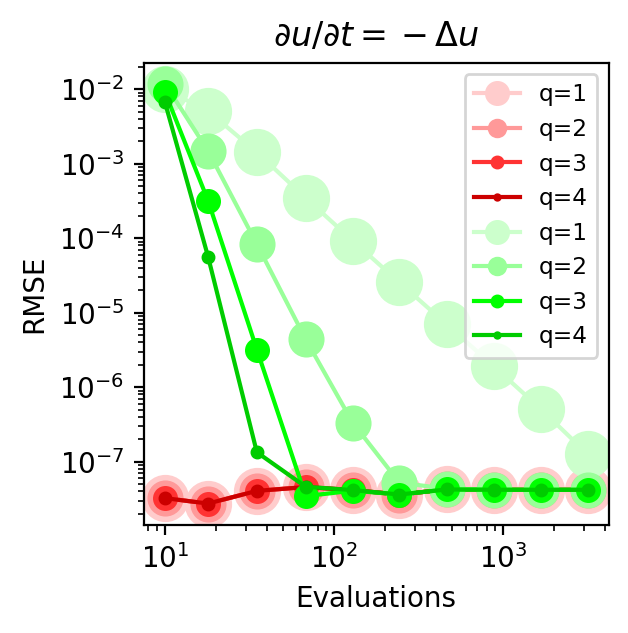
\includegraphics[width=\columnwidth]{../images/solver_heat.png}
    \caption{}
    \label{fig:heat}
    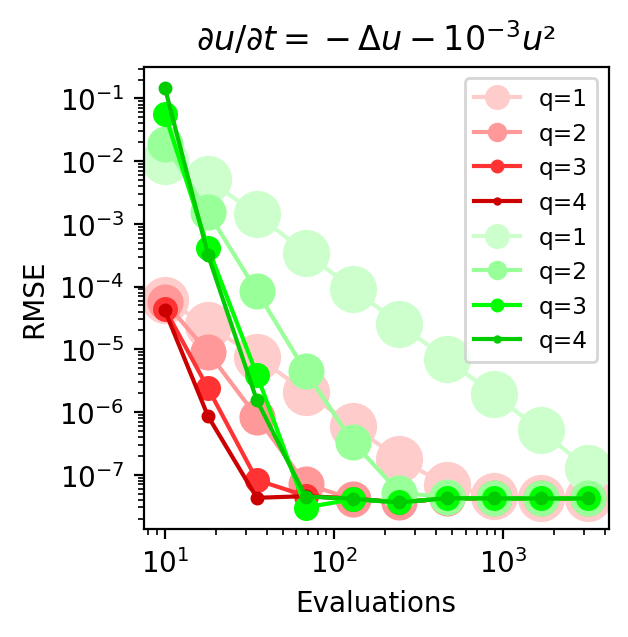
\includegraphics[width=\columnwidth]{../images/solver_heat and medium square.png}
    \caption{}
    \label{fig:heat medium}
    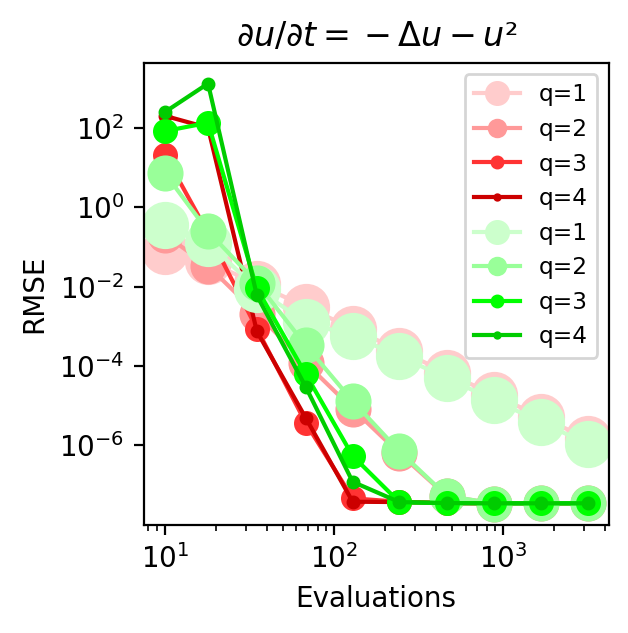
\includegraphics[width=\columnwidth]{../images/solver_heat and big square.png}
    \caption{}
    \label{fig:heat big}
\end{figure}
\begin{figure}
    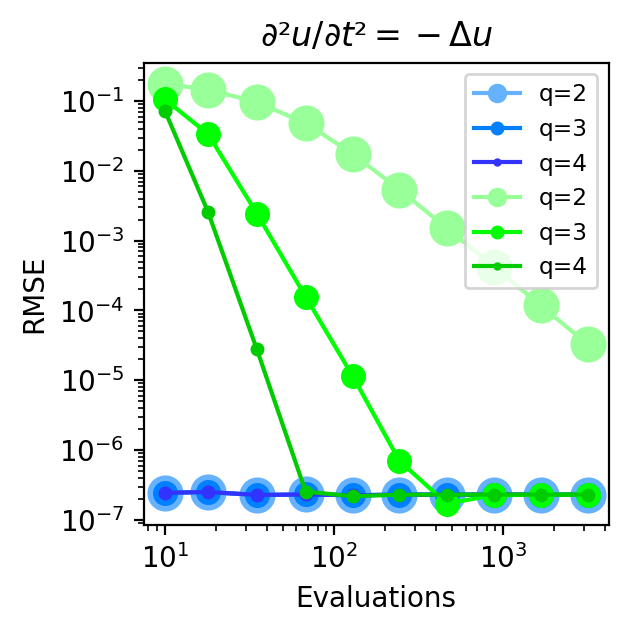
\includegraphics[width=\columnwidth]{../images/solver_wave.png}
    \caption{}
    \label{fig:wave}
    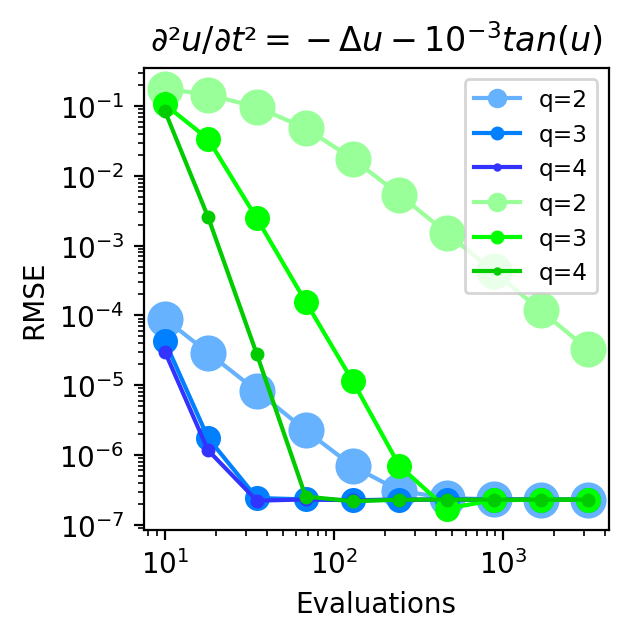
\includegraphics[width=\columnwidth]{../images/solver_wave and medium tan.png}
    \caption{}
    \label{fig:wave medium}
    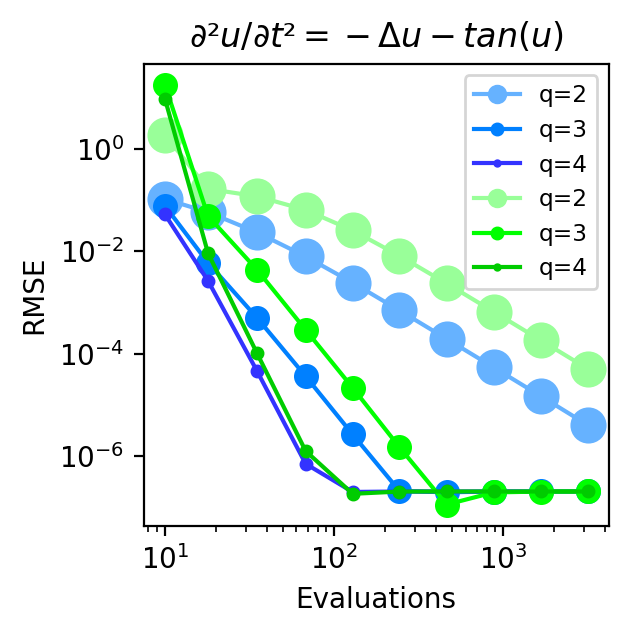
\includegraphics[width=\columnwidth]{../images/solver_wave and big tan.png}
    \caption{}
    \label{fig:wave big}
\end{figure}


\ifdefined\COMPILINGFROMMAIN
\else    
    \end{document}
\fi

\section{Conclusion}
  
\printbibliography

\end{document}
